\documentclass[11pt,twoside]{report}

\usepackage{fts-report}
\usepackage{siunitx}
\usepackage{booktabs}
\usetikzlibrary{positioning, matrix, calc}
\usetikzlibrary{arrows.meta}

\title{2026 Digital Chemistry}
\author{F. T. Szczypiński}
\date{Michaelmas Term 2026}

\addbibresource{refs.bib}

% Student version: leave gaps blank
% \solutionsfalse
% Lecturer version: display worked answers
\solutionsfalse

\begin{document}
\begin{titlepage}
\thispagestyle{empty}

\vspace*{2.5cm}

\noindent

\begin{tcolorbox}[
  enhanced,
  colback=white,
  colframe=white,
  boxrule=0pt,
  arc=0pt,
  left=10pt,
  right=30pt,
  top=10pt,
  bottom=10pt,
  height=2cm,
  width=1.2\textwidth,
  valign=center,
  borderline east={8pt}{0pt}{darkBlue}
]
{\sffamily\bfseries\fontsize{36}{42}\color{darkBlue}\selectfont
\raggedleft\MakeUppercase{Digital Chemistry}\par}
\end{tcolorbox}

\begin{tcolorbox}[
  enhanced,
  colback=white,
  colframe=white,
  boxrule=0pt,
  arc=0pt,
  left=10pt,
  right=30pt,
  top=10pt,
  bottom=10pt,
  height=1.2cm,
  width=1.2\textwidth,
  valign=center,
  borderline east={8pt}{0pt}{darkBlue!80}
]
{\raggedleft\sffamily\Huge\color{darkBlue!80}
Michaelmas Term 2026\par}
\end{tcolorbox}

\vfill

\begin{tcolorbox}[
  enhanced,
  colback=white,
  colframe=white,
  boxrule=0pt,
  arc=0pt,
  left=10pt,
  right=30pt,
  top=10pt,
  bottom=10pt,
  height=1.5cm,
  width=1.2\textwidth,
  valign=center,
  borderline east={8pt}{0pt}{darkBlue}
]
{\raggedleft\sffamily\Huge\bfseries\color{darkBlue}
Dr Filip Szczypiński\par}
\end{tcolorbox}

\begin{tcolorbox}[
  enhanced,
  colback=white,
  colframe=white,
  boxrule=0pt,
  arc=0pt,
  left=10pt,
  right=30pt,
  top=10pt,
  bottom=10pt,
  height=1cm,
  width=1.2\textwidth,
  valign=center,
  borderline east={8pt}{0pt}{darkBlue!60}
]
{\raggedleft\sffamily\LARGE\color{darkBlue!60}
filip.t.szczypinski@durham.ac.uk\par}
\end{tcolorbox}

\end{titlepage}

\tableofcontents

\raggedbottom

% % !TeX root = ../notes.tex

\chapter*{About this course}
\addcontentsline{toc}{chapter}{About this course}

\section*{What this course will achieve}
This course connects physical organic chemistry, cheminformatics, data analysis, reaction optimisation and laboratory automation. Its central question is how chemists can translate molecules and experiments into structured data, extract chemical understanding from those data, and use that understanding to choose and perform better experiments.

\section*{What is digital chemistry?}
In this course, \emph{digital chemistry} means the use of machine-readable molecular and experimental information to support chemical understanding and experimental decision-making. It includes molecular representations, chemical-space analysis, quantitative physical organic methods, machine learning, optimisation, automated experimentation and closed-loop laboratories. It is not treated as a replacement for chemical reasoning: the objective is to make chemical reasoning quantitative, reproducible and scalable.

\begin{warningbox}
\textbf{Scope:} digital chemistry is broader than artificial intelligence, and automation alone does not make an experiment autonomous.
\end{warningbox}

\section*{Learning outcomes}
By the end of the course, students should be able to:
\begin{enumerate}
  \item compare common molecular representations;
  \item explain how descriptors define different chemical spaces;
  \item interpret VTNA and RPKA plots mechanistically;
  \item distinguish regression, classification, and optimisation problems;
  \item assess model validation, and chemical usefulness;
  \item compare OVAT, design of experiments and Bayesian optimisation;
  \item explain how to generate structured chemical data;
  \item design a conceptual closed-loop workflow that balances chemical performance, sustainability and experimental constraints.
\end{enumerate}

\section*{Case-study threads}
\begin{itemize}
  \item \textbf{Physical organic chemistry:} asymmetric catalysis, non-linear effects, kinetics, RPKA and VTNA.
  \item \textbf{Green chemistry:} solvent selection, process mass intensity, multi-objective optimisation and responsible automation.
  \item \textbf{Cheminformatics:} molecular representations, fingerprints, similarity, descriptors and molecular libraries.
\end{itemize}

\begin{insightbox}
\textbf{Recurring question:} what information is needed, how should it be represented, and what chemical decision will it support?
\end{insightbox}

\begin{conceptbox}
  Concept box
\end{conceptbox}

\begin{warningbox}
  Warning box
\end{warningbox}

\begin{methodbox}
  Method box
\end{methodbox}

\begin{resultbox}
  Result box
\end{resultbox}

\begin{notebox}
  Note box
\end{notebox}
% !TeX root = ../notes.tex

\chapter{Translating molecules for computers}


\section{Information in chemical structures}

Chemists routinely communicate molecular structure using drawings.
A skeletal formula can encode a considerable amount of information in a compact form because we have learnt conventions for interpreting atoms, bonds, functional groups and stereochemistry.
Consider a simple example of proline (Fig.~\ref{fig1-1:proline}) and what information we implicitly capture about its structure.

\begin{figure}[h!]
    \centering
    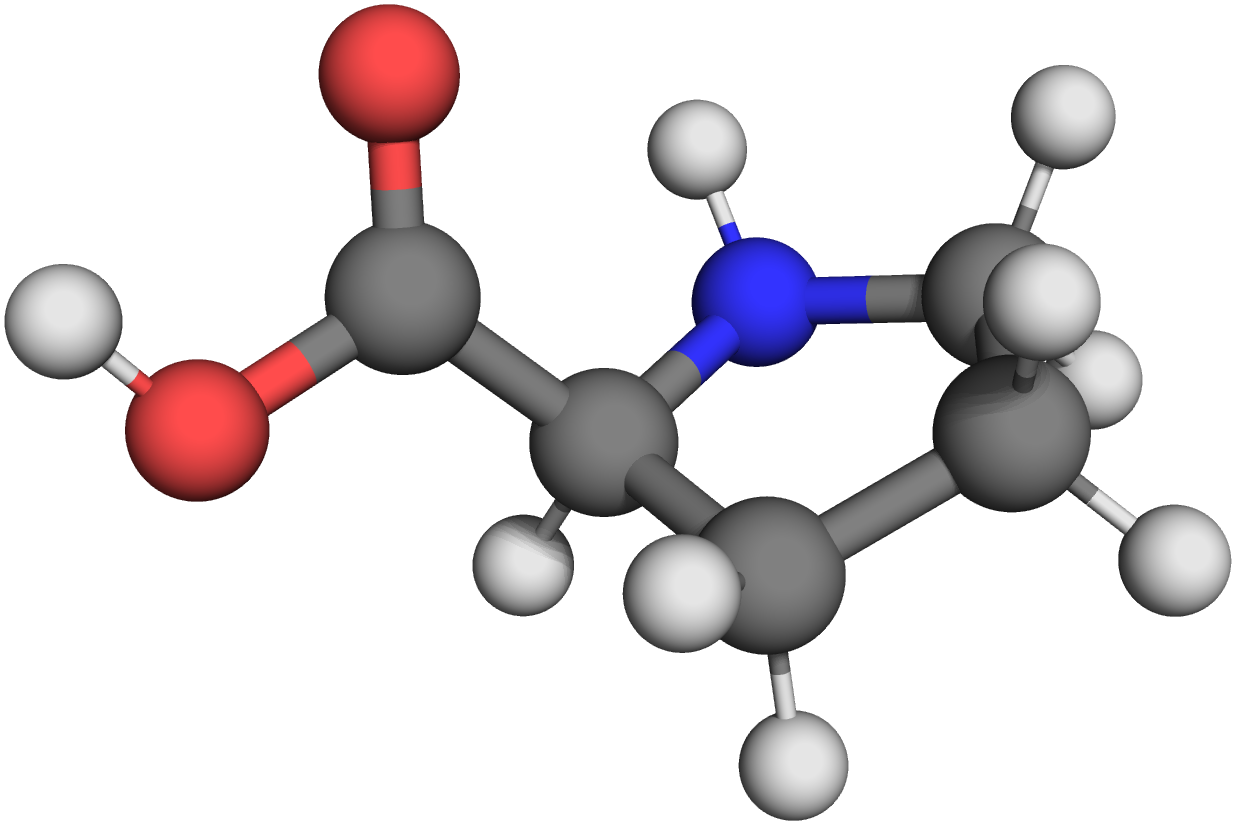
\includegraphics[width=8.3cm]{figures/CH1-01-proline.png}
    \caption{Molecular structure of proline.}
    \label{fig1-1:proline}
\end{figure}

\solution{5.5cm}{
    \begin{itemize}
        \item atoms (incl. implicit hydrogens)
        \item connectivity and bond orders
        \item functional groups
        \item stereochemistry
        \item protonation
        \item \dots
    \end{itemize}
}

Computers do not interpret chemical drawings in the same way.
To store, search, compare and analyse molecules computationally, chemical information must first be represented in a form that can be processed by computer algorithms.

\begin{conceptbox}
\textbf{Main question:} how should we represent a molecule to a computer?
\end{conceptbox}

Throughout this chapter, we will encounter several ways of representing molecules digitally. 
These range from three-dimensional atomic coordinates to text strings, identifiers and numerical fingerprints.
Rather than asking which representation is \enquote{best}, we will ask \keypoint{what chemical information each representation contains}, what it discards, and what it allows us to do.

The information required by a computer depends on the task.
A calculation of molecular geometry requires the positions of atoms in three-dimensional space.
A substructure search requires information about atoms and their connectivity.
Searching a database for a particular chemical requires a consistent identifier.
Comparing the structural similarity of thousands of compounds requires a representation that can be compared efficiently.
Consequently, the same molecule may be represented in several different ways within a single workflow.

\begin{resultbox}
    \textbf{For each task below, consider what information must be retained:} \vspace{0.5em}
    \begin{itemize}
        \item calculate the distance between two atoms;
        \item determine whether a molecule contains a substructure;
        \item find a compound in a database;
        \item compare a molecule with one million other structures.
    \end{itemize}
\end{resultbox}

\section{Coordinates and molecular geometry}

One of the most direct ways of describing a geometry is to specify the position of every atom in three-dimensional space, often in a simple \texttt{.xyz} file (Lst.~\ref{lst1-1:xyz-proline}).
The first line contains the number of atoms, followed by molecule name, and its coordinates.
Other filetypes (\emph{e.g.}, \texttt{.mol2}) might also include bonding information.

\begin{listing}
\begin{codebox}{bash}
17
Proline
   H       -0.13097       -1.07655        1.63572
   C       -0.15726       -0.63902        0.60818
   C       -1.20401       -1.38526       -0.20437
   O       -1.15189       -1.78305       -1.35456
   O       -2.35852       -1.64177        0.45250
   H       -2.96245       -2.10328       -0.12133
   N        1.22788       -0.77675        0.06680
   C        1.69088        0.54717       -0.43489
   H        2.56627        0.82982        0.18087
   H        2.04876        0.49358       -1.48090
   C        0.54048        1.53722       -0.27264
   H        0.08541        1.78163       -1.25139
   H        0.88732        2.50157        0.14048
   C       -0.47304        0.86447        0.64762
   H       -1.51350        1.08299        0.34489
   H       -0.38097        1.24444        1.68280
   H        1.28559       -1.47722       -0.63981
\end{codebox}
\caption{Proline geometry as an \texttt{.xyz} file.}
\label{lst1-1:xyz-proline}
\end{listing}

For a molecule, a Cartesian representation assigns three coordinates, $(x_i,y_i,z_i)$ for each atom $i$.
Those are often represented using \keypoint{internal coordinates} (\textit{e.g.}, bond lengths, bond angles, and dihedral angles) in a \emph{Z-matrix}.
However, even such explicit representation might miss important details required for calculations, \textit{e.g.,} overall charge and spin multiplicity (Lst.~\ref{lst1-1:orca-proline}).


\begin{listing}
\begin{codebox}{bash}
! B3LYP D3BJ def2-TZVP OPT FREQ

* xyzfile 0 1 proline.xyz
\end{codebox}
\caption{An ORCA input file for a geometry optimisation calculation of proline.}
\label{lst1-1:orca-proline}
\end{listing}

Now, consider the two structures of proline in Figure~\ref{fig1-2:prolines} -- are they the same molecule?
A useful molecular representation should not change just because we move or rotate a molecule in space.

\begin{figure}[h!]
    \centering
    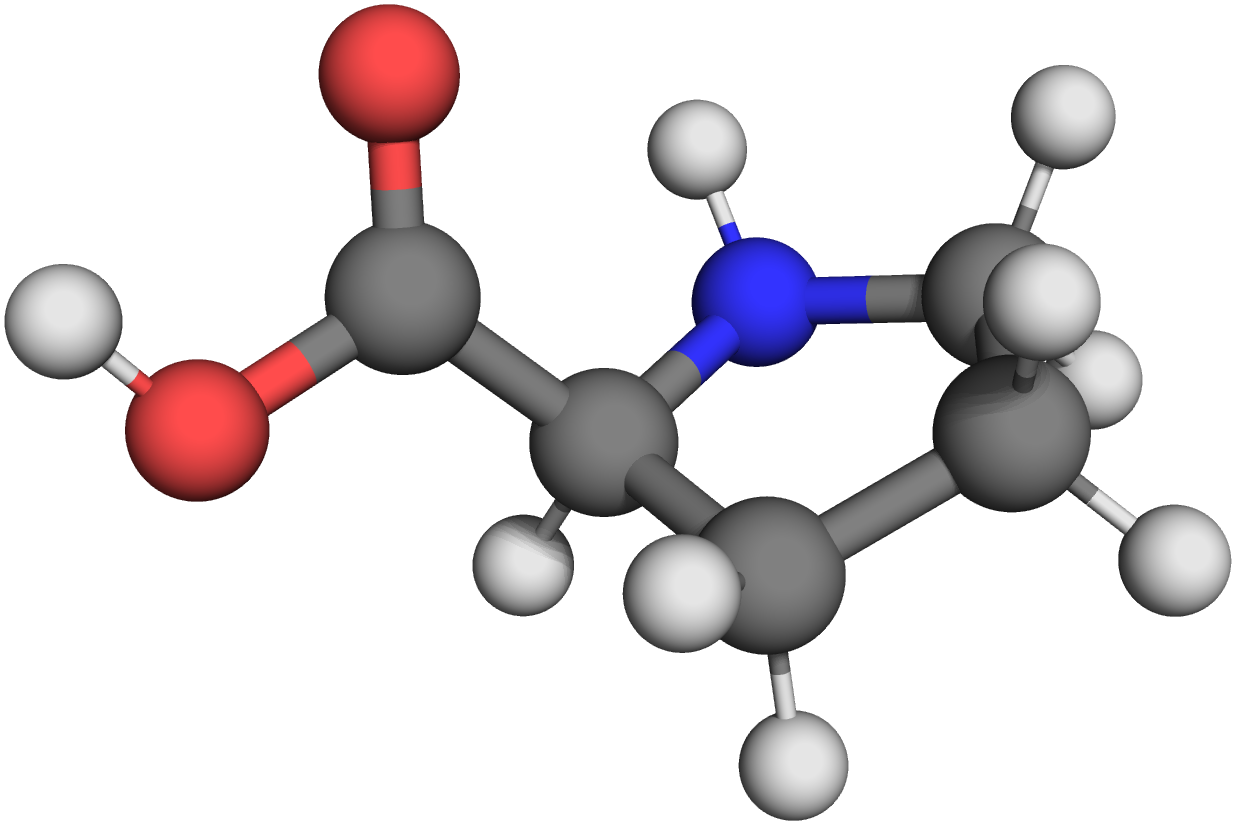
\includegraphics[width=6.4cm]{figures/CH1-01-proline.png}
    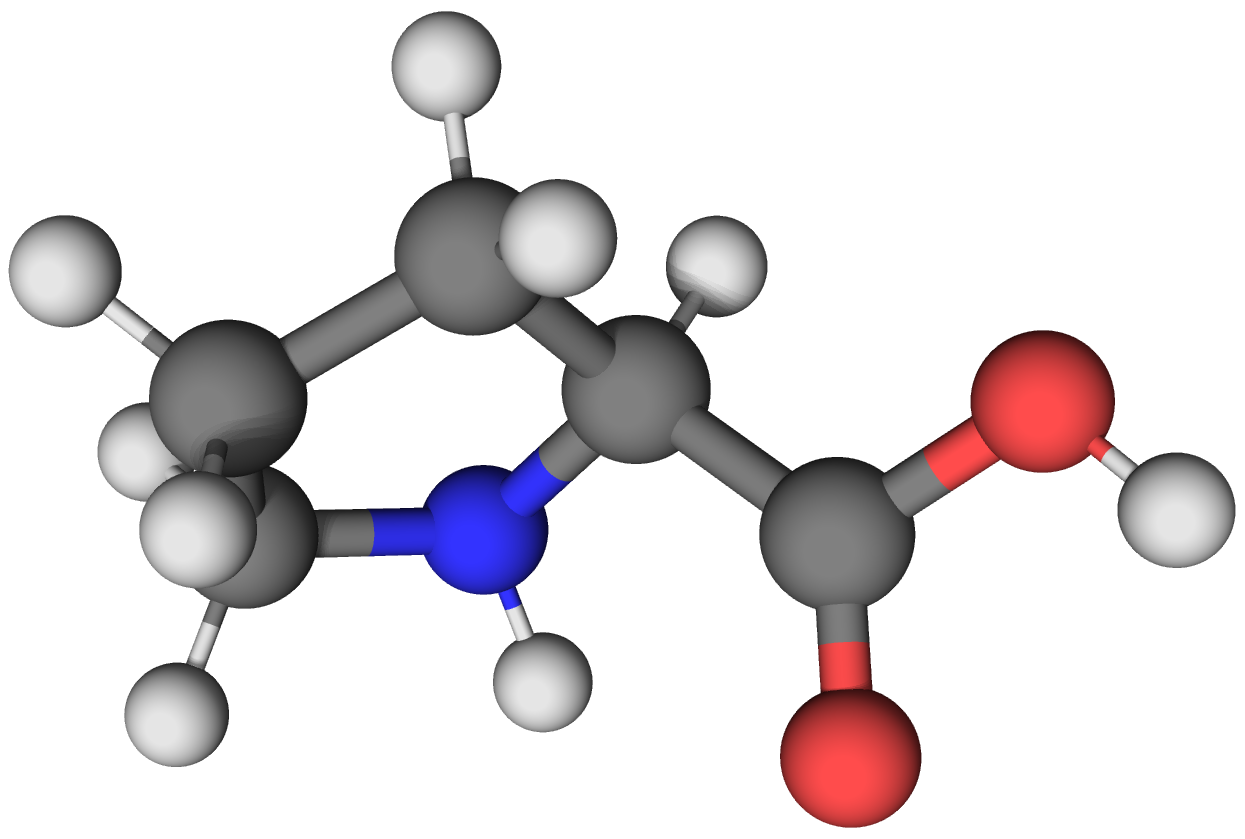
\includegraphics[width=6.4cm]{figures/CH1-02-proline.png}
    \caption{Two equivalent molecular structures of proline with different atomic coordinates.}
    \label{fig1-2:prolines}
\end{figure}

One way to retain information about both atomic identity and molecular geometry upon rotation is the \keypoint{Coulomb matrix}.\mcite{Rupp2012} 
For atoms with nuclear charges \(Z_i\) and Cartesian positions \(\mathbf{R}_i\),

\begin{equation}
    C_{ij} = \begin{cases} 
        \frac{1}{2}Z_i^{2.4} & \mathrm{for} \quad i=j,\\[6pt] 
        \frac{Z_iZ_j}{|\mathbf R_i-\mathbf R_j|} & \mathrm{for} \quad i\ne j. 
    \end{cases}
\end{equation}

Because the off-diagonal elements depend only on interatomic distances, translating or rotating the molecule does not change Coulomb matrix.
\mnote{The exponent 2.4 is empirical rather than fundamental:
the diagonal term approximates the energy of an isolated atom.}
Reordering the atoms permutes the rows and columns of the matrix.
The matrix itself is therefore not invariant to atom ordering, but its \keypoint{sorted eigenspectrum} is:

\begin{equation}
    \mathbf{λ} = (λ_1,λ_2,\ldots,λ_N) 
    \qquad 
    \textrm{where} 
    \qquad 
    λ_1\geqλ_2\geq\cdots\geqλ_N.
\end{equation}

\begin{warningbox} 
    \textbf{Invariant does not mean unique:} 
    the Coulomb matrix eigenspectrum removes dependence on molecular orientation and atom ordering, but different molecular structures can share the same eigenspectrum.
    It is, therefore, not necessarily a unique molecular identifier. 
\end{warningbox}

Consider a water molecule with the following Cartesian coordinates (in \(\si{\angstrom}\)): 

\begin{center}
    \begin{tabular}{crrr} 
        \toprule 
        Atom & \(x\) & \(y\) & \(z\) \\
        \midrule 
        O & 0.0000 & 0.0000 & 0.0000 \\ 
        H & 0.9572 & 0.0000 & 0.0000 \\ 
        H & -0.2400 & 0.9273 & 0.0000 \\ 
        \bottomrule
    \end{tabular} 
\end{center} 


\solution{18cm}{ 
    Using \(Z_{\mathrm{O}}=8\) and \(Z_{\mathrm{H}}=1\).
    \\[3em]
    The interatomic distances are approximately 
    
    \[ r_{\mathrm{OH_1}} = 0.9572~\si{\angstrom}, \qquad r_{\mathrm{OH_2}} = 0.9578~\si{\angstrom}, \qquad r_{\mathrm{H_1H_2}} = 1.514~\si{\angstrom}. \] 
    
    The diagonal oxygen term is 
    
    \[ C_{\mathrm{OO}} = \frac{1}{2}(8)^{2.4} = 73.517, \] 
    
    while each hydrogen diagonal term is 
    
    \[ C_{\mathrm{HH}} = \frac{1}{2}(1)^{2.4} = 0.500. \] The resulting Coulomb matrix is approximately \[ \mathbf{C} = \begin{pmatrix} 73.517 & 8.358 & 8.352 \\ 8.358 & 0.500 & 0.660 \\ 8.352 & 0.660 & 0.500 \end{pmatrix}. \] 

    The eigenvalues are the values of \(λ\) satisfying \[ \det(\mathbf C-λ\mathbf I)=0. \]
    
    Its eigenvalues, sorted from largest to smallest, are 
    
    \[ \boldsymbol{\lambda} = \begin{pmatrix} 75.397\\ -0.160\\ -0.720 \end{pmatrix}. \] 
}

\section{Molecules as graphs} 

Three-dimensional representations are essential when the geometry of a molecule matters.
For many chemical problems, however, we are primarily interested in which atoms are connected to which (\keypoint{molecular topology}).
This motivates representing a molecule as a \keypoint{molecular graph} (Fig.~\ref{fig1-3:proline-graph}).

A mathematical graph consists of a collection of \keypoint{vertices} connected by \keypoint{edges}.
Molecular structure maps naturally onto this representation: atoms become vertices and bonds become edges.
A molecular graph can contain more information than connectivity alone.
Properties can be attached to both atoms and bonds.
Such a graph is sometimes described as an \keypoint{attributed graph}.

\begin{figure}[htbp]
\centering
\begin{tikzpicture}[
    vertex/.style={
        circle,
        draw=darkBlue,
        fill=paleBlue,
        minimum size=9mm,
        inner sep=1pt,
        font=\sffamily\bfseries,
        line width=1.5pt
    },
    edge/.style={
        draw=darkGrey,
        line width=2pt
    },
    doubleedge/.style={
        draw=darkGrey,
        double,
        double distance=2.4pt,
        line width=2pt
    },
    index/.style={
        font=\small\sffamily,
        text=darkGrey
    }
    ]

    % Proline pyrrolidine ring arranged as a regular-looking pentagon
    \node[vertex] (N)  at (0,1.65) {N};
    \node[vertex] (Ca) at (1.57,0.51) {C};
    \node[vertex] (Cb) at (0.97,-1.34) {C};
    \node[vertex] (Cg) at (-0.97,-1.34) {C};
    \node[vertex] (Cd) at (-1.57,0.51) {C};

    % Carboxylic acid attached to alpha carbon
    \node[vertex] (Cc) at (3.25,1.10) {C};
    \node[vertex] (O1) at (4.45,2.20) {O};
    \node[vertex] (O2) at (4.75,0.35) {O};

    % Curved pyrrolidine ring edges
    \draw[edge] (N) to[bend left=7] (Ca);
    \draw[edge] (Ca) to[bend left=7] (Cb);
    \draw[edge] (Cb) to[bend left=7] (Cg);
    \draw[edge] (Cg) to[bend left=7] (Cd);
    \draw[edge] (Cd) to[bend left=7] (N);

    % Curved carboxylic acid edges
    \draw[edge] (Ca) to[bend left=6] (Cc);
    \draw[doubleedge] (Cc) to[bend left=7] (O1);
    \draw[edge] (Cc) to[bend right=7] (O2);

    % Arbitrary graph indices
    \node[index,above=1mm of N] {1};
    \node[index,right=1mm of Ca] {2};
    \node[index,right=1mm of Cb] {3};
    \node[index,below=1mm of Cg] {4};
    \node[index,left=1mm of Cd] {5};
    \node[index,above=1mm of Cc] {6};
    \node[index,above=1mm of O1] {7};
    \node[index,right=1mm of O2] {8};

\end{tikzpicture}

\caption{
    Hydrogen-suppressed molecular graph of proline.
    Atomic identity is represented as a vertex attribute and bond order as an edge attribute.
    The numerical vertex indices are arbitrary.
}
\label{fig1-3:proline-graph}
\end{figure}

Once the vertices of a molecular graph have been assigned indices, the connectivity of the graph can itself be represented numerically.
For a simple, unweighted molecular graph, the \keypoint{adjacency matrix} \(\mathbf{A}\) is defined as
\mnote{We could define different numerical values for edge attributes.}

\begin{equation} 
    A_{ij} = \begin{cases} 
        1, & \text{if vertices } i \text{ and } j \text{ are connected},\\ 
        0, & \text{otherwise}. 
    \end{cases} 
\end{equation}

\solution{6cm}{
    \[ \mathbf{A} = \begin{pmatrix} 0 & 1 & 0 & 0 & 1 & 0 & 0 & 0 \\ 1 & 0 & 1 & 0 & 0 & 1 & 0 & 0 \\ 0 & 1 & 0 & 1 & 0 & 0 & 0 & 0 \\ 0 & 0 & 1 & 0 & 1 & 0 & 0 & 0 \\ 1 & 0 & 0 & 1 & 0 & 0 & 0 & 0 \\ 0 & 1 & 0 & 0 & 0 & 0 & 1 & 1 \\ 0 & 0 & 0 & 0 & 0 & 1 & 0 & 0 \\ 0 & 0 & 0 & 0 & 0 & 1 & 0 & 0 \end{pmatrix}. \] 
}

\section{Line notations}

Molecular graphs provide a convenient abstract representation of chemical connectivity, but explicitly storing and displaying a graph is not always practical.
An alternative is to encode the molecular graph as a sequence of characters. Such \keypoint{line representations} allow molecular structures to be stored, searched and exchanged using ordinary text.
The most widely encountered example is the \keypoint{S}implified \keypoint{M}olecular \keypoint{I}nput \keypoint{L}ine \keypoint{E}ntry \keypoint{S}ystem, or \keypoint{SMILES}.\mcite{Weininger1988}

\subsection{SMILES syntax}

Atoms are represented using their element symbols.
Adjacent atoms in the string are connected by a bond.
Hydrogen atoms attached to typical organic atoms are normally omitted and inferred from standard valence rules.
Single bonds are normally omitted, so for ethanol: 
\begin{equation} 
    \ce{C-C-O} \qquad\longrightarrow\qquad \texttt{CCO} 
\end{equation} 
Double and triple bonds are written explicitly using an equals sign (\texttt{O=C=O} is carbon dioxide) and a hash symbol (\texttt{C\#C} is acetylene).
A branch in the molecular graph is written inside parentheses following the atom (\texttt{CC(=O)N} is acetamide).

\solution{12.5cm}{
    \centering
    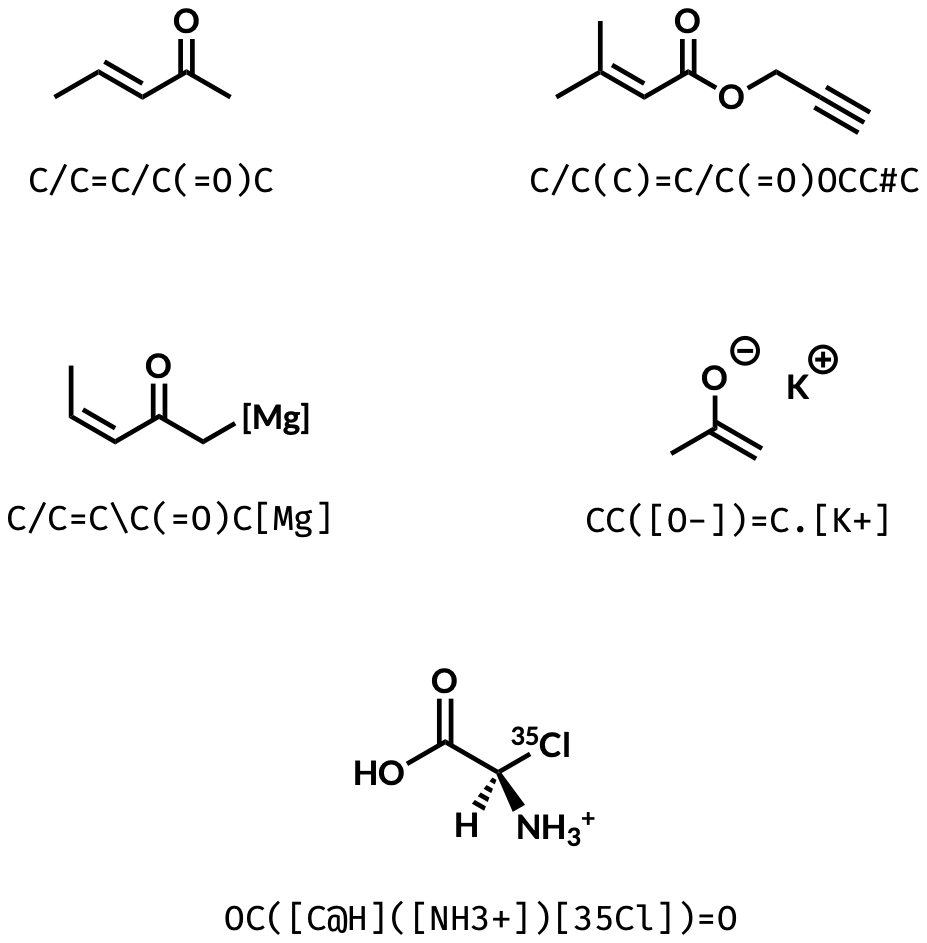
\includegraphics[width=8cm]{figures/CH1-smiles-1.png}
}

A cyclic molecular graph cannot be represented simply by walking along a sequence of atoms without eventually reconnecting two vertices. 
SMILES indicates this \keypoint{ring closure} using matching numerical labels.
Aromatic atoms can be represented either as Kekulé structure or with lower-case letters.

\begin{warningbox} 
    \keypoint{The ring number does not represent an atom.} 
    Matching ring labels indicate the edge connecting two atoms encountered during the graph traversal.
\end{warningbox}

\solution{8cm}{
    \centering
    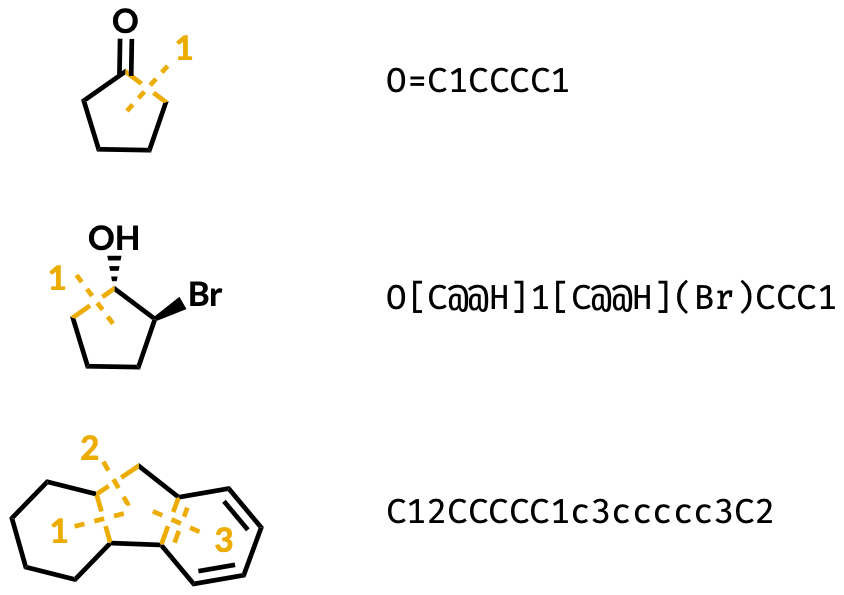
\includegraphics[width=8cm]{figures/CH1-smiles-2.png}
}

A molecular graph can usually be traversed in more than one way.
Consequently, a single molecule can have multiple valid SMILES representations.

\solution{8cm}{
    \centering
    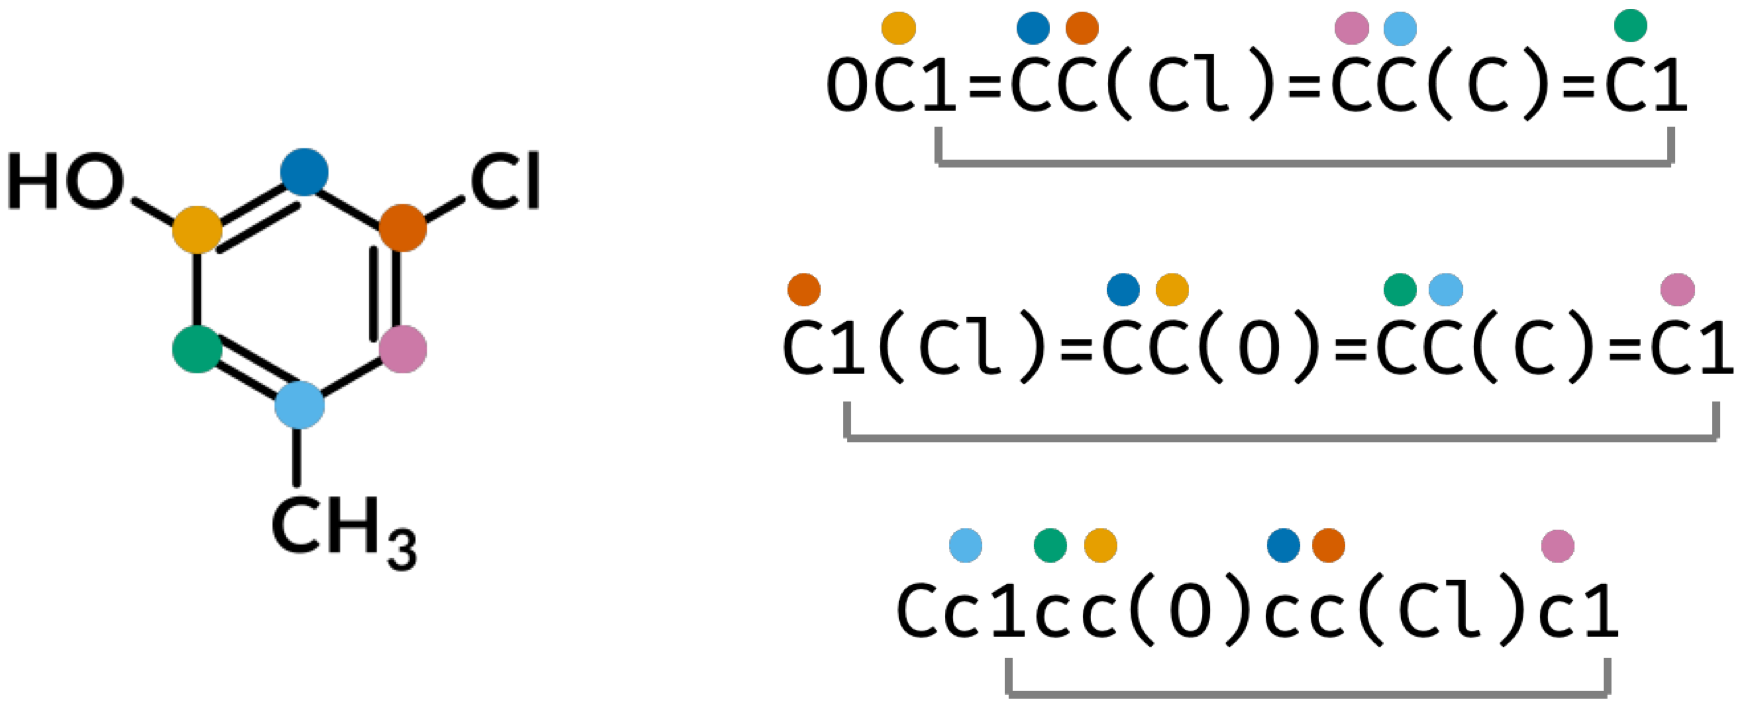
\includegraphics[width=8cm]{figures/CH1-smiles-3.png}
}

For database searching and comparison, having many valid strings for the same molecular graph is inconvenient.
A \keypoint{canonicalisation algorithm} assigns a reproducible ordering to the graph and generates a corresponding canonical SMILES.

\begin{warningbox} 
    \keypoint{Canonical does not mean universal.} 
    Canonical SMILES are generated algorithmically. 
    Different software packages can employ different canonicalisation procedures, so the same molecule need not have one universally defined canonical SMILES.
    These can even vary between software versions!
\end{warningbox}

Several related line notations extend or modify the ideas used in SMILES. 
\keypoint{SMARTS} describes a molecular pattern rather than one specific molecule. 
It is used for substructure searching, allowing questions such as whether a molecule contains an alcohol, amide or aromatic nitrogen atom.
\keypoint{SMIRKS} encodes a chemical transformation by specifying patterns in the reactants and the corresponding patterns in the products. 
\keypoint{SELFIES} is a string representation designed so that every valid SELFIES string corresponds to a molecular graph permitted by its underlying rules.\mcite{Krenn2020} 
This makes SELFIES useful in generative machine learning, where arbitrary modification of a SMILES will often produce an invalid structure.

\section{Identifiers and chemical records}

SMILES strings can also contain special characters that are inconvenient when structures are passed between different pieces of software or used as search terms.
More fundamentally, the existence of multiple valid SMILES representations makes them inconvenient as universal chemical identifiers for cross-referencing structures from different sources.
For searching databases and linking chemical information between different sources, it is useful to have a standardised molecular identifier.

\subsection{The International Chemical Identifier (InChI)}

To address these problems, IUPAC developed the \keypoint{International Chemical Identifier (InChI)}.\mcite{Heller2015}
InChI is a structure-based, non-proprietary, open-source, and standardised identifier in which different types of chemical information are organised hierarchically into layers. 
This makes InChI particularly useful when chemical information from different sources needs to be linked or incorporated into \keypoint{FAIR} (\keypoint{f}indable, \keypoint{a}ccessible, \keypoint{i}nteroperable, and \keypoint{r}eusable) datasets.

\begin{conceptbox}
    \keypoint{An InChI is organised into layers of chemical information.} 
    An InChI begins with a version identifier and molecular formula, followed by additional layers describing features such as connectivity, hydrogen atoms, charge, stereochemistry, and isotopic composition.
    Layers are included only where the corresponding information is required to describe the structure.
\end{conceptbox}

The ability to read and parse InChI by humans was of little importance to the developers.
You are not expected to construct an InChI manually. 
You should, however, be able to recognise the organisation of an InChI and identify where important types of chemical information are stored (Fig.~\ref{fig1-4:inchi}).

\begin{figure}[h!]
    \centering
    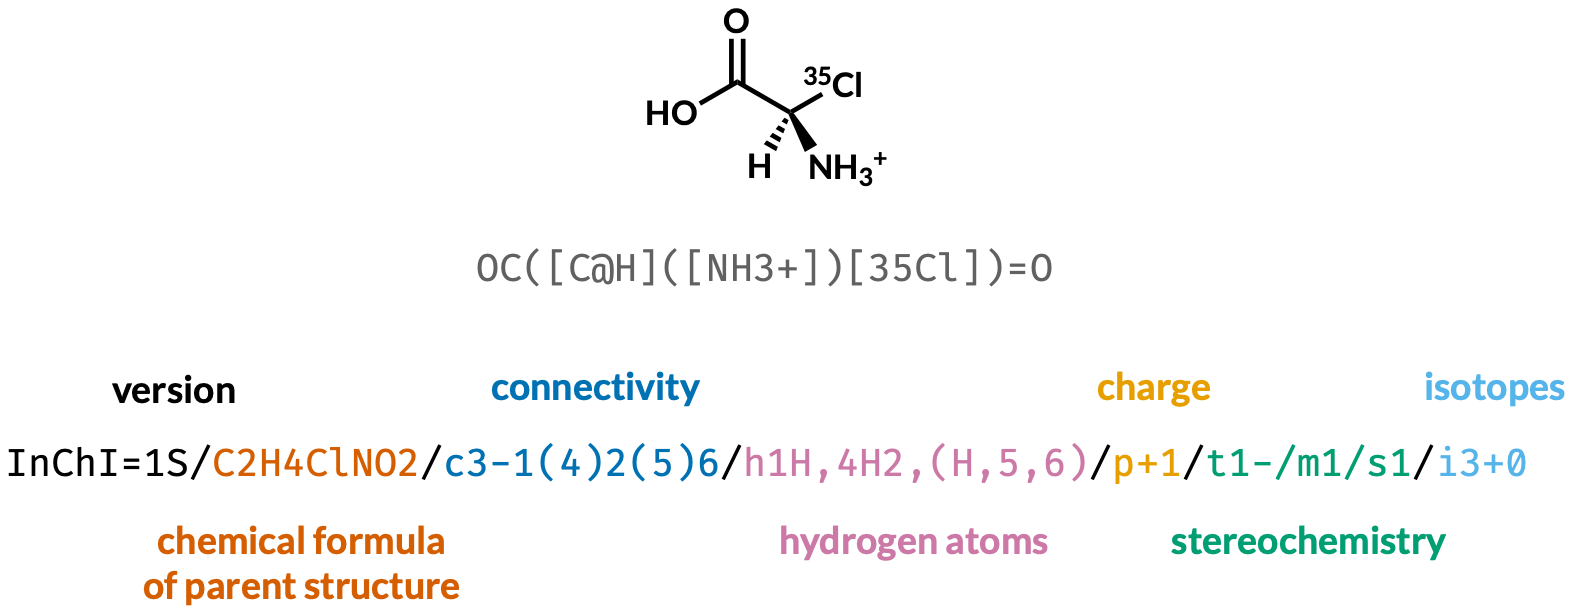
\includegraphics[width=\textwidth]{figures/CH1-inchi-1.png}
    \caption{An example chemical structure with its corresponding InChI. Note how each layer gives more and more chemical information.}
    \label{fig1-4:inchi}
\end{figure}

\subsection{Search engines and indexing}

Although InChIs provide standardised identifiers, they can have varying lengths and contain characters that are inconvenient for search engines, database indexing and filenames.
For this reason, a second identifier, the \keypoint{InChIKey}, can be generated from the InChI.
An InChIKey is a hash of an InChI that produces a compact 27-character identifier containing uppercase letters and hyphens (Fig.~\ref{fig1-5:inchikey}).

\begin{figure}[h!]
    \centering
    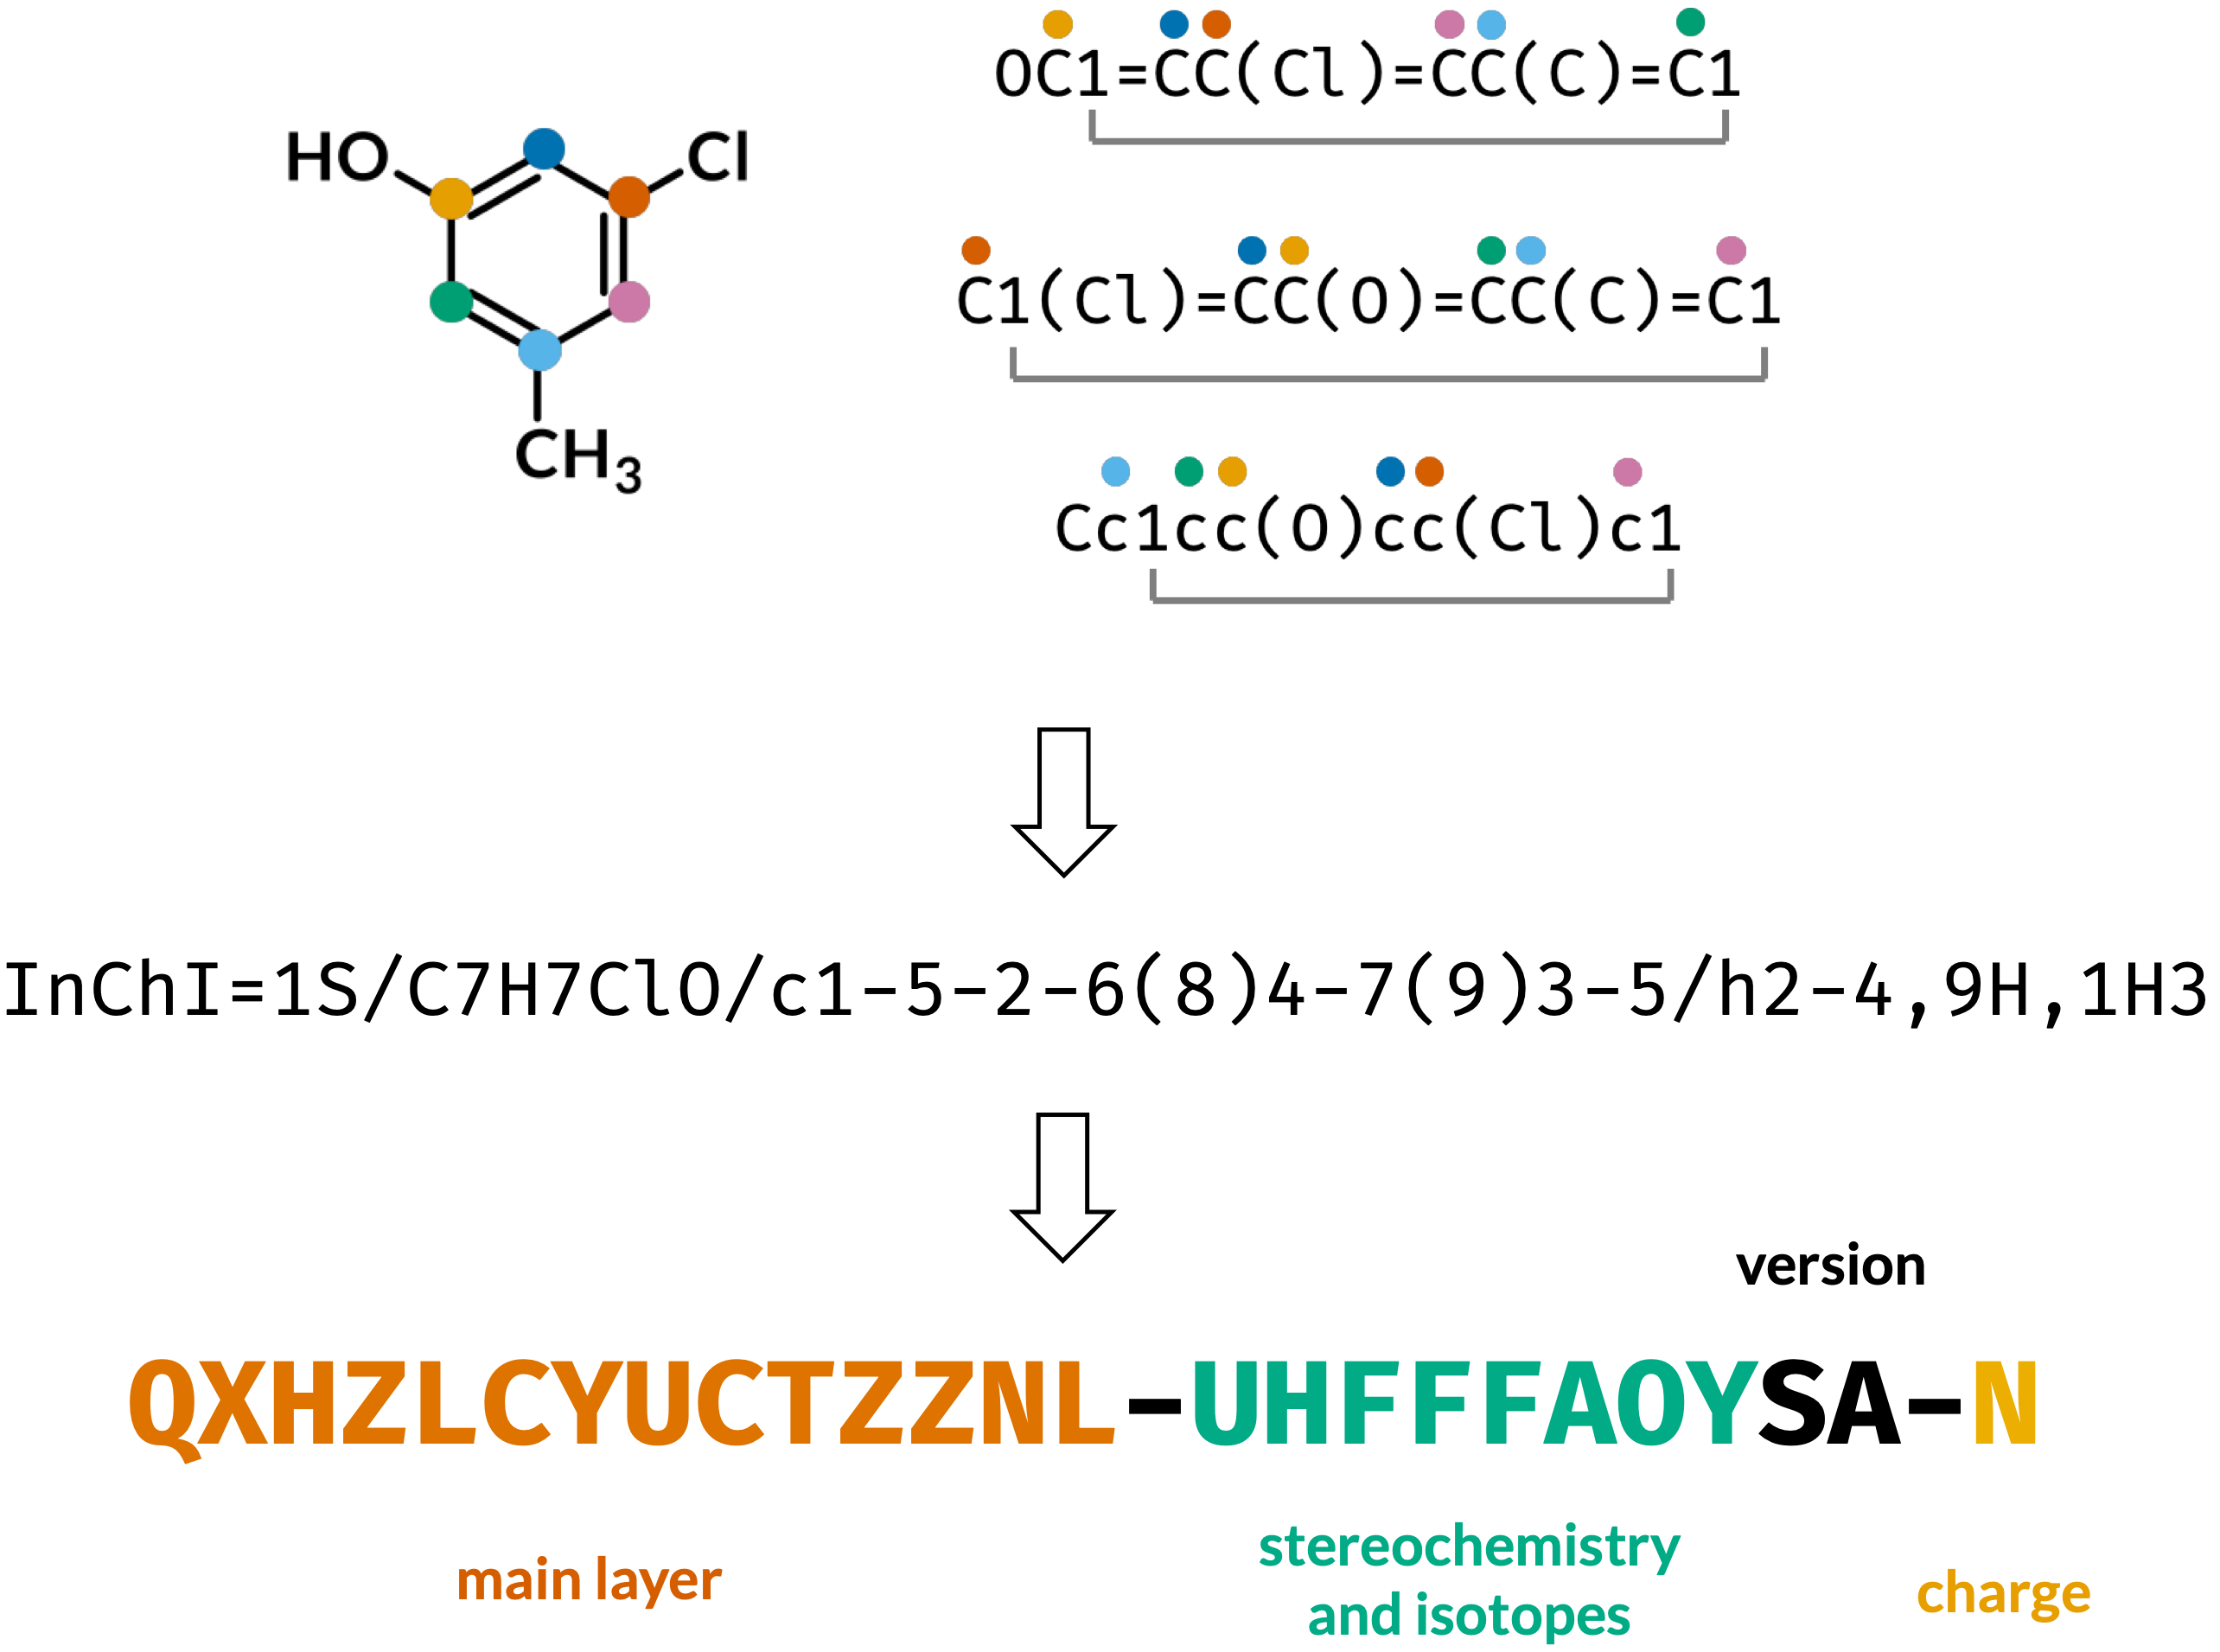
\includegraphics[width=12.5cm]{figures/CH1-inchikey.png}
    \caption{Different molecular representations of the same molecule: non-unique SMILES, standardised InChIn and its corresponding InChIKey.}
    \label{fig1-5:inchikey}
\end{figure}

\begin{warningbox}
    Hashing is a one-way operation. 
    The same InChI will reproducibly generate the same InChIKey, but it is not possible to recover the complete molecular structure from the InChIKey alone.
    While they are convenient filenames, it is wise keep a \enquote{dictionary} mapping them to structural information.
\end{warningbox}

The InChIKey is divided into blocks. 
The first block represents information associated primarily with the connectivity, while subsequent parts encode information associated with stereochemistry, isotopic composition and protonation.

\solution{8cm}{
    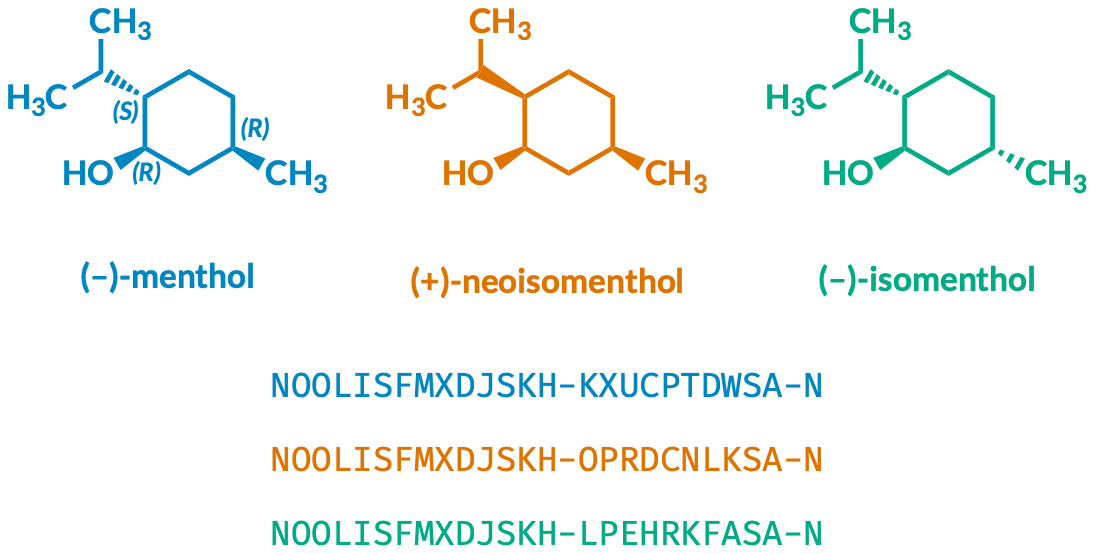
\includegraphics[width=12.5cm]{figures/CH1-inchikey-chiral.png}
}

Compressing an InChI into a much shorter InChIKey necessarily loses information.
This creates the possibility of a \emph{hash collision}, in which different InChIs generate the same InChIKey.
While the \texttt{SHA-256 hash} was chosen to minimise collisions of InChIKeys, they are still possible -- especially for large structures. 
Consider two diastereomers of Spongistatin I, a molecule with 26 stereocentres, which have different InChI but the same InChIKey (Fig.~\ref{fig1-6:inchikey-collision}).
Such collisions are incredibly rare, but it is prudent to check they have not happened in our datasets!

\begin{figure}[h!]
    \centering
    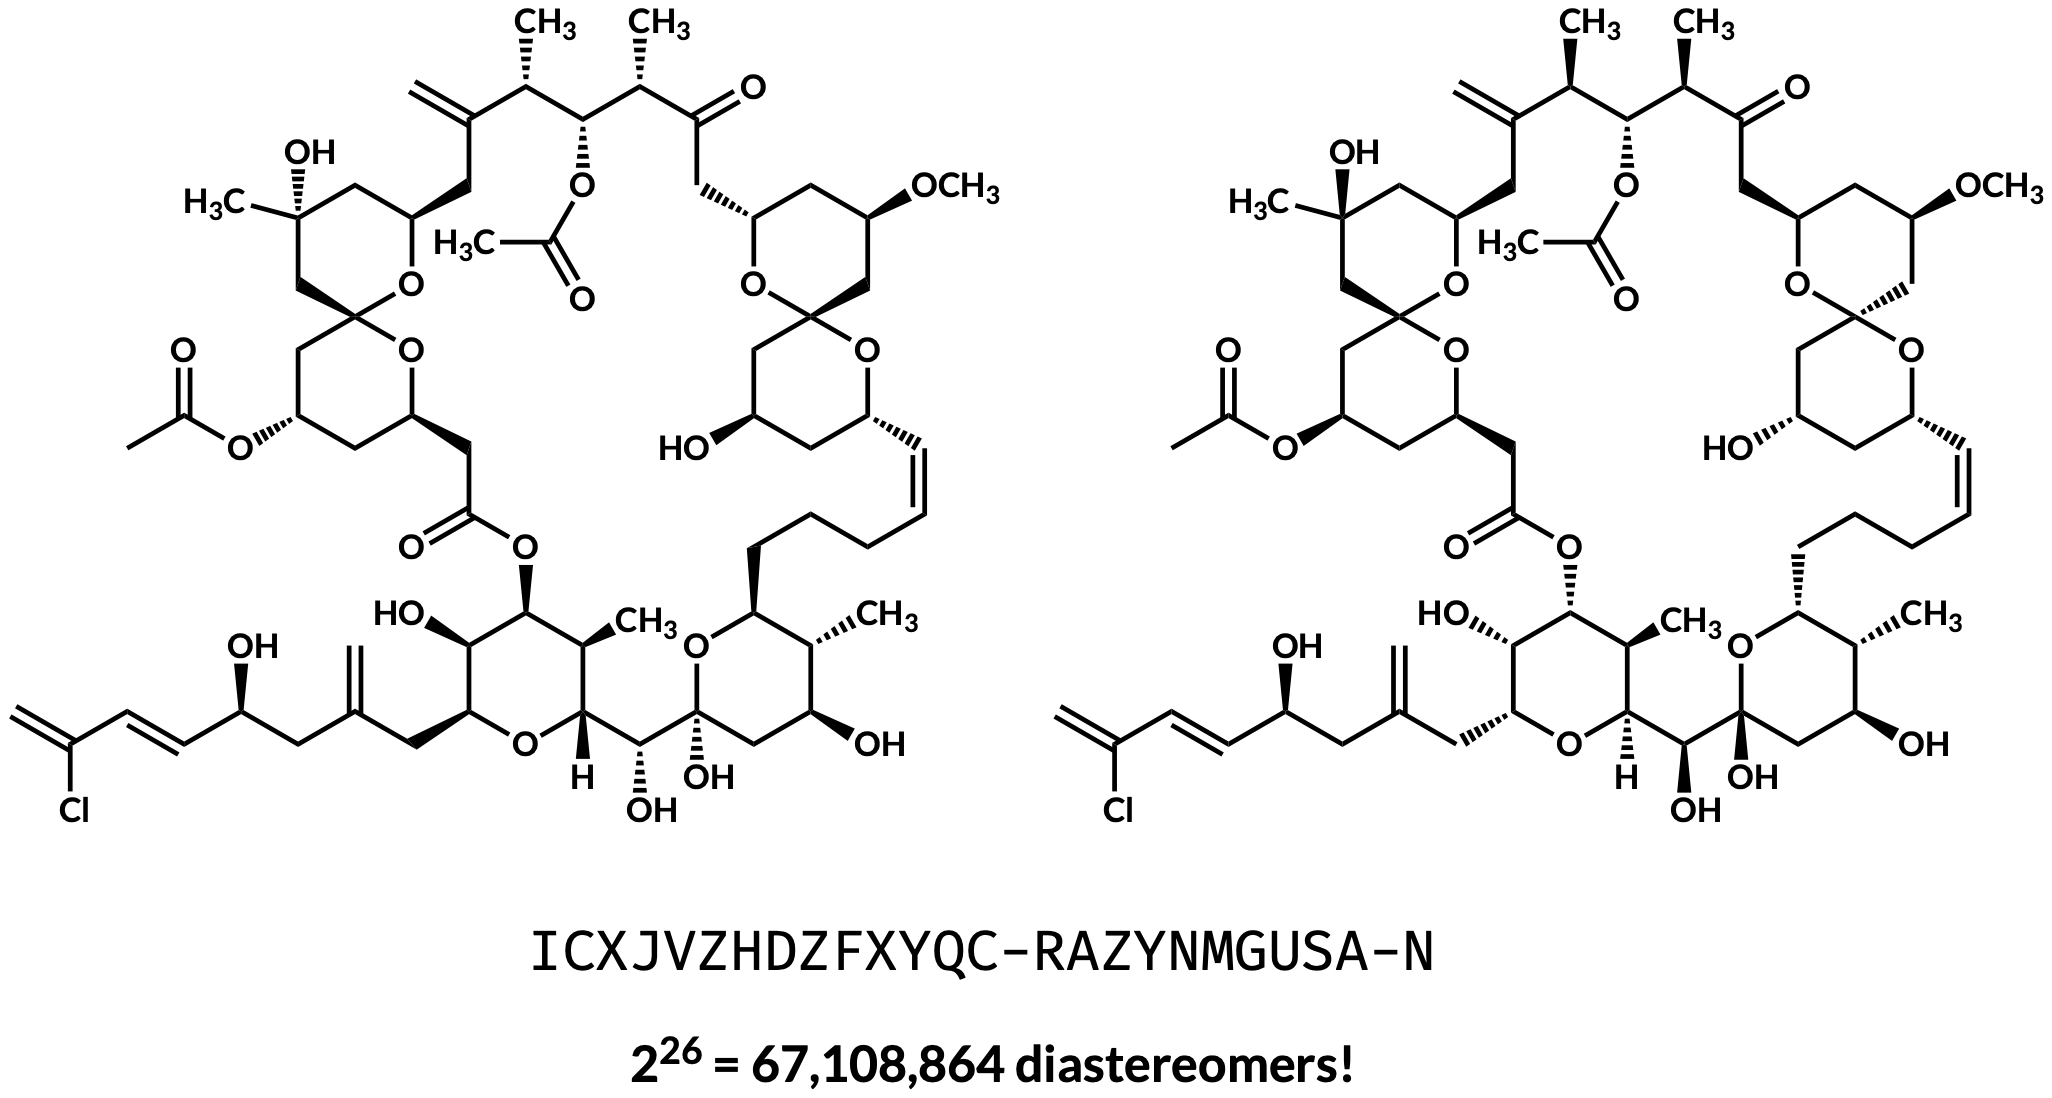
\includegraphics[width=\textwidth]{figures/CH1-inchikey-collision.png}
    \caption{Two diastereomers of Spongistatin I with the same InChIKey.}
    \label{fig1-6:inchikey-collision}
\end{figure}

\section{Bit vectors and molecular fingerprints}

So far, we have considered representations that aim to describe or identify a molecular structure. 
For many cheminformatics applications, however, we do not need to reconstruct the complete structure of a molecule. 
Instead, we may want to answer much simpler questions: does a particular structural feature occur in the molecule, and how similar is one molecule to another?
For these tasks, it is useful to convert molecular structures into compact numerical representations known as \keypoint{molecular fingerprints}.

A \keypoint{bit vector} is a one-dimensional array containing zeros and ones, for example,

\begin{equation} 
    \mathbf{x} = (0,0,1,1,0,1). 
\end{equation}

Each position, or \emph{bit}, can be used to record the presence or absence of some feature of a higher-dimensional object such as a molecule.
This might initially seem an unnecessarily crude way of representing chemical structure. 
However, identifying and comparing substructures directly across very large molecular databases can be computationally expensive.
Once molecules have been converted into bit vectors, computers can compare their patterns of zeros and ones extremely efficiently.

\begin{conceptbox} 
    \keypoint{Molecular fingerprints trade detail for computational efficiency.}
    A molecular fingerprint encodes selected features of a molecular structure in a compact numerical form. 
    It is generally not possible to reconstruct the complete molecular structure from the fingerprint.
\end{conceptbox}

\subsection{Structural keys}

One simple way to construct a such a bit vector is to define a fixed list of yes/no structural questions. 
Each question is assigned a position in the bit vector, and the corresponding bit is switched on if the feature is present.
A very simple list of such structural questions could be:
\begin{itemize} 
    \item does the molecule contain oxygen? 
    \item does it contain a ring? 
    \item does it contain an aromatic atom? 
    \item does it contain a six-membered ring? 
    \item does it contain a carbonyl group? 
\end{itemize}

\begin{methodbox} \keypoint{A structural-key fingerprint asks a predefined set of questions about a molecule.}
Each structural feature is associated with a particular bit:
\begin{equation*} 
    \begin{aligned} 
        \text{feature absent} &\longrightarrow 0 \\ 
        \text{feature present} &\longrightarrow 1
    \end{aligned} 
\end{equation*}

Two molecules sharing many of the encoded structural features will consequently share many \enquote{on} bits, which can be cheaply compared.
\end{methodbox}

One widely used example is the \keypoint{M}olecular \keypoint{ACC}ess \keypoint{S}ystem (\keypoint{MACCS}) structural key fingerprint.\mcite{Durant2002}
MACCS keys use a predefined collection of 167 (of which one is not implemented) structural patterns intended to summarise useful information about molecular structure (Fig.~\ref{fig1-7:maccs}).

\begin{figure}[h!]
    \centering
    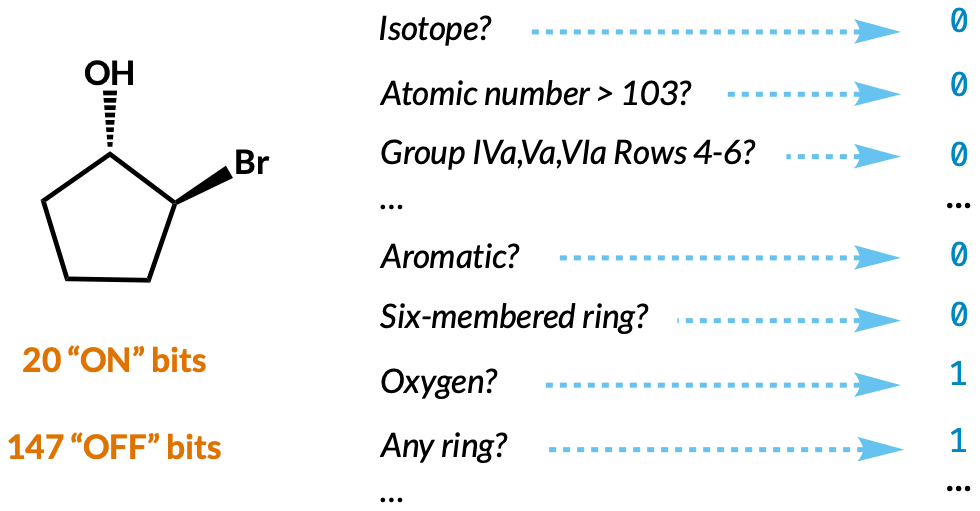
\includegraphics[width=0.8\textwidth]{figures/CH1-maccs.png}
    \caption{Example MACCS keys for a simple organic molecule.}
    \label{fig1-7:maccs}
\end{figure}

Someone must decide in advance which structural patterns are worth encoding. 
A set of keys designed for one region of chemistry may fail to capture the structural distinctions that matter in another.

\subsection{Circular fingerprints}

Rather than deciding in advance which structural patterns are important, we can generate features directly from the molecular graph.
\keypoint{Circular fingerprints} describe the local environment surrounding each atom and progressively expand that environment through neighbouring atoms:
\begin{enumerate} 
    \item assign an initial identifier to each atom; 
    \item identify the neighbouring atoms and bonds; 
    \item combine this information to describe larger local environments; 
    \item convert each environment into a numerical identifier; 
    \item encode the resulting identifiers in a fingerprint. 
\end{enumerate}
The size of an atomic environment is described by its \keypoint{radius}. 
At radius 0, the environment describes the atom itself. 
Radius 1 additionally includes directly bonded neighbours, radius 2 extends to the next shell of atoms, and so forth (Fig.~\ref{fig1-8:morgan}).
Increasing the radius incorporates progressively more of the local molecular environment surrounding each atom.

\begin{figure}[h!]
    \centering
    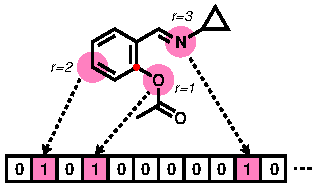
\includegraphics[width=0.8\textwidth]{figures/CH1-morgan-1.pdf}
    \caption{Conceptual representation of a circular fingerprint.}
    \label{fig1-8:morgan}
\end{figure}

One of the most widely used approaches to circular fingerprints derives from the Morgan algorithm introduced by the Chemical Abstracts Society (CAS).
A more recent development of this idea is the \keypoint{Extended-Connectivity Fingerprint (ECFP)}.\mcite{Rogers2010}
For each atom, the algorithm generates identifiers describing its local molecular environments.
These identifiers can then be \keypoint{hashed}: a numerical operation converts an identifier into an integer, which can subsequently be mapped onto a position in a fingerprint of fixed length through modulo division (Fig.~\ref{fig1-8:morgan-2}).
If the same structural environment occurs in another molecule, the same procedure generates the same identifier and therefore maps to the same position in the fingerprint.
Different substructures can give rise to the same bits, so while a fingerprint can easily confirm the absence of a substructure, it does not indicate any certainty that the substructure is indeed present.
These \keypoint{hash collisions} is what you see in spurious substructures in CAS~SciFinder.

\begin{conceptbox} 
    \keypoint{Morgan fingerprints describe which local molecular environments occur within a molecular graph.}
    Unlike predefined structural keys, those environments do not need to be chosen before the molecules are analysed, making circular fingerprints useful across a wide range of chemical datasets.
\end{conceptbox}

\begin{figure}[h!]
    \centering
    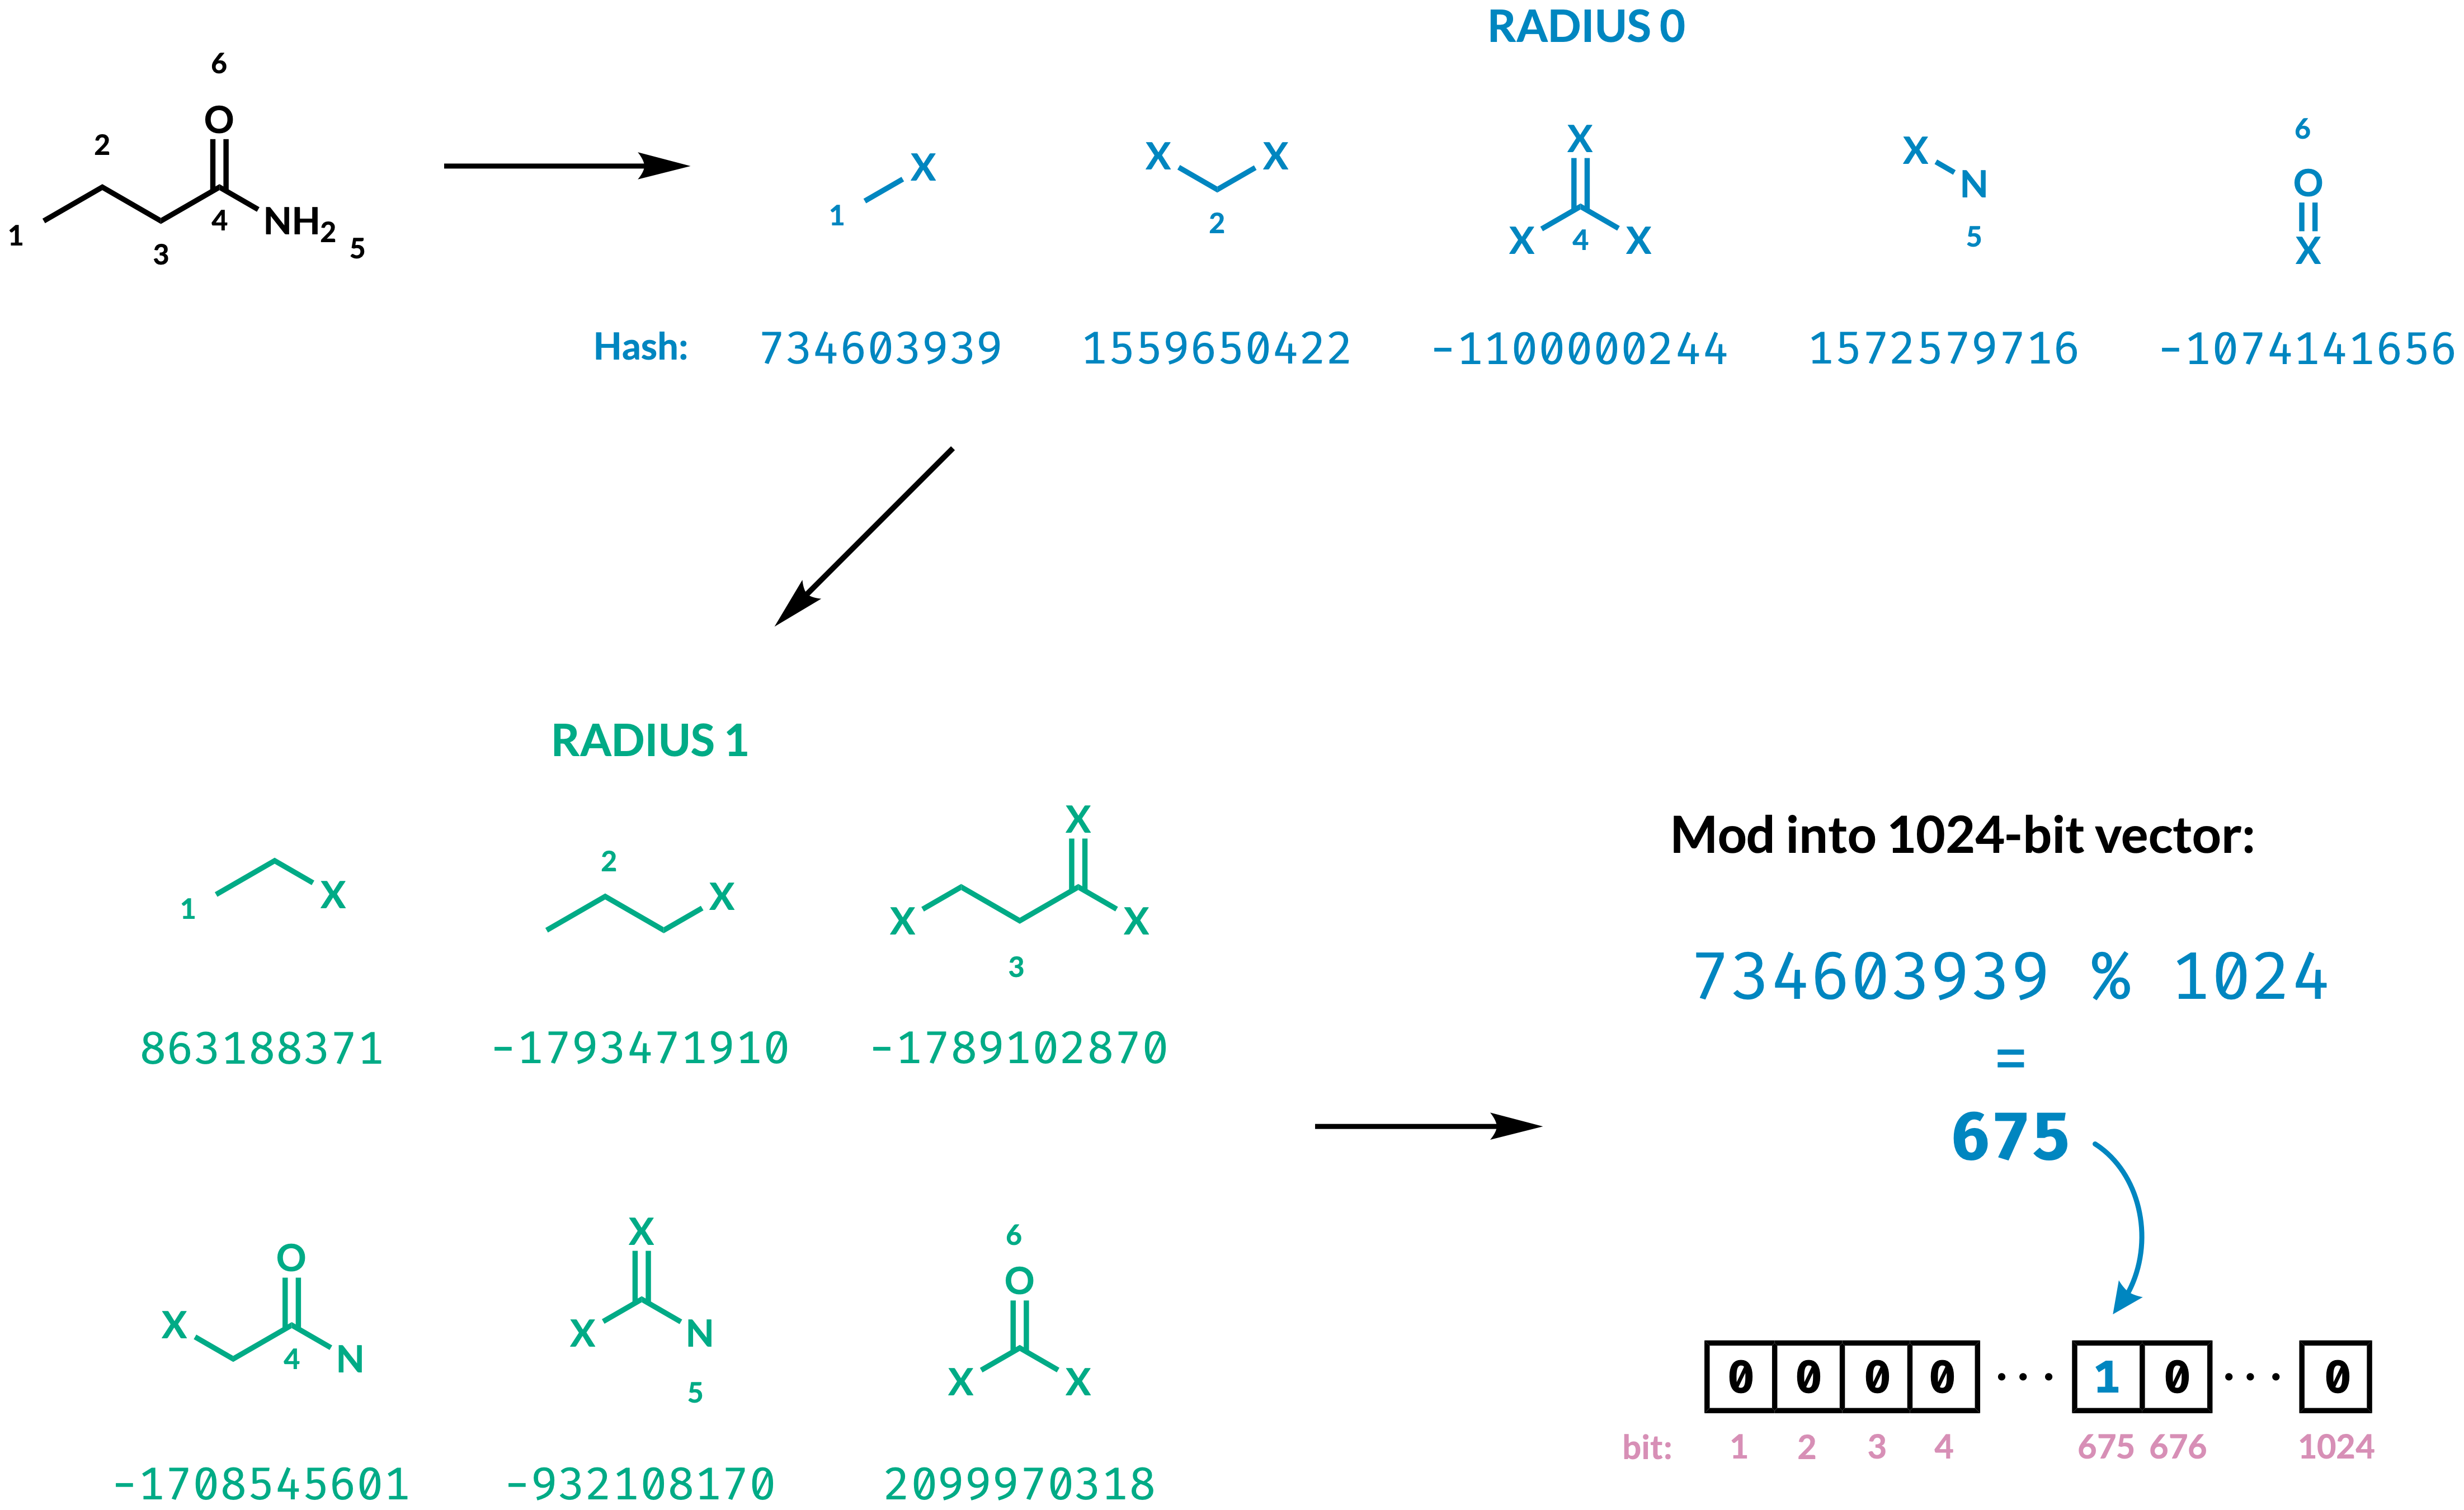
\includegraphics[width=\textwidth]{figures/CH1-morgan-2.png}
    \caption{
        Generation of an ECFP fingerprint with contributions from environments up to radius one. 
        Bits activated by each environment are based on the hashing function.
    }
    \label{fig1-8:morgan-2}
\end{figure}

A binary fingerprint records only whether a feature occurs:
\begin{equation} 
    x_i\in{0,1}. 
\end{equation}
An alternative is a \keypoint{count fingerprint}, in which each position records how many times a feature occurs within the molecule:
\begin{equation} 
    x_i\in{0,1,2,\ldots}. 
\end{equation}
Count fingerprints therefore retain information that is deliberately discarded when a bit is simply switched on.
Extended-connectivity fingerprints normally distinguish atomic environments using atom-specific information. 
A related representation, the \keypoint{Functional-Class Fingerprint (FCFP)}, instead groups atoms according to chemically relevant roles, such as hydrogen-bond donor or acceptor, aromatic character, or membership of broader functional classes.

\section{Summary}

In this chapter, we have seen that a molecule can be represented digitally in many different ways, and that \keypoint{there is no universally \enquote{best} molecular representation}.
Instead, the appropriate representation depends on the chemical information that must be retained and the task we want to perform.
Cartesian coordinates provide detailed information about \keypoint{molecular geometry}, while molecular graphs abstract a structure into its \keypoint{atoms and connectivity}.
Line representations such as SMILES provide a compact way of encoding molecular graphs as text, while InChI and InChIKey provide standardised approaches to \keypoint{chemical identification and data interoperability}.
Finally, molecular fingerprints deliberately discard some structural information to produce compact numerical representations that are efficient to store and compare.
These representations therefore illustrate a recurring theme in digital chemistry: \keypoint{the choice of representation determines which chemical information is made explicit, which information is hidden, and which information is lost}.
Having learnt how to represent individual molecules, we can now ask a different question: if molecules are represented computationally, \keypoint{how can we decide how similar or different they are?}
Answering this question takes us from individual molecular representations to the organisation and exploration of the \keypoint{chemical space}.


% !TeX root = ../notes.tex

\chapter{Machine learning for chemistry}

\begin{notebox}
  \keypoint{What do you need to learn from this chapter?}
  This chapter introduces the language and basic ideas of machine learning that will be used throughout the remainder of the course.
  You are \keypoint{not} expected to derive machine-learning algorithms, implement the models discussed here, or reproduce their mathematical details in the exam.
  You should instead understand the \keypoint{conceptual vocabulary}: what features and targets are, the difference between regression and classification, what it means to train and test a model, and why ideas such as overfitting and extrapolation matter when interpreting chemical models.
  Later chapters will use these concepts to address chemical questions.
\end{notebox}

\section{Learning relationships from data}

Machine learning (ML) has become increasingly common across chemistry, from predicting molecular properties and reaction outcomes to selecting experiments and controlling automated laboratories.\mcite{Butler2018}
Despite the terminology, many of the underlying ideas should already be familiar to chemists: we collect observations, identify variables that might explain them, construct a model, and ask whether that model can describe or predict chemical behaviour.
The principal difference is often one of \keypoint{scale}.
Rather than considering a single relationship between two variables, machine-learning methods can identify relationships within datasets containing many observations and many molecular or experimental variables

Consider a dataset in which each row represents a chemical reaction.
For every reaction, we might record information about the substrates, catalyst, solvent, temperature, concentration, and measured reaction outcome.
Some of these quantities can be provided to a model as inputs, while another quantity can be treated as the value that we would like the model to predict.
An \keypoint{observation} is one example in a dataset.
In chemistry this might be one molecule, one reaction, or one experiment.
A \keypoint{feature} is an input variable used to describe an observation.
Examples might include temperature, Hammett parameters, catalyst loading, or solvent properties.
A \keypoint{target} is the quantity that we want the model to predict, such as a reaction rate, selectivity, or yield.
\keypoint{Training} is the process by which a model learns a relationship between features and a target from existing data.
\keypoint{Prediction} uses the resulting model to estimate the target for new observations.

The terminology is relatively new to many chemists, but the underlying idea is not.
A physical-organic relationship such as a Hammett correlation also relates a numerical description of molecular structure to an experimentally observed chemical quantity.
Before constructing any model we must decide what constitutes an observation, which chemical information should be supplied as features, and which experimentally meaningful quantity should be treated as the target.
Later in this course, we will see how this idea can be extended to many molecular descriptors and more complicated chemical relationships.

\section{Types of machine-learning problem}

Machine-learning problems can be divided into several broad classes according to the information available during training and the type of question being asked.

\subsection{Supervised learning}

In \keypoint{supervised learning}, the training data contain both the features describing each observation and the correct value or label that the model is intended to learn (Fig.~\ref{fig2-1:supervised-learning}).
For example, we might provide a model with molecular and experimental features for a collection of reactions together with the experimentally measured selectivity of each reaction.
The model attempts to learn a relationship between these inputs and outputs that can subsequently be applied to new reactions.

Two important supervised-learning problems are \keypoint{regression} and \keypoint{classification}.
Regression is used when the target is a \keypoint{continuous numerical quantity}.
Chemical examples might include:

\begin{itemize}
  \item reaction rate;
  \item activation free energy, \(ΔG^\ddagger\);
  \item selectivity, \(ΔΔG^\ddagger\);
  \item a molecular property;
  \item percentage yield.
\end{itemize}

Classification is used when the target belongs to one of a set of \keypoint{discrete categories}.
For example, reactions might be classified as reactive or unreactive, or a chemical sample might be assigned to one of several predefined classes.
Converting a continuous chemical measurement into categories inevitably discards information.
For example, dividing reactions into \enquote{high yield} and \enquote{low yield} requires an arbitrary boundary.

\begin{figure}[htbp]
  \centering

  \resizebox{\linewidth}{!}{%
    \begin{tikzpicture}[
        transform shape,
        box/.style={
          draw=darkBlue,
          fill=paleBlue,
          line width=2.0pt,
          minimum width=5cm,
          minimum height=1.2cm,
          align=center,
          font=\sffamily
        },
        model/.style={
          draw=darkRed,
          fill=paleRed,
          line width=2.0pt,
          minimum width=5cm,
          minimum height=1.2cm,
          align=center,
          font=\sffamily
        },
        result/.style={
          draw=darkGreen,
          fill=paleGreen,
          line width=2.0pt,
          minimum width=5cm,
          minimum height=1.2cm,
          align=center,
          font=\sffamily
        },
        arrow/.style={
          ->,
          >=Stealth,
          draw=darkGrey,
          line width=2.5pt
        }
      ]

      % Fix the natural width so that both figures receive the same
      % scaling factor when resized to \linewidth.
      \path[use as bounding box] (0,-1.9) rectangle (17.3,3.8);

      \node[box] (training) at (2.5,3)
      {
        \textbf{Training data}\\
        features + known target
      };

      \node[model] (algorithm) at (8.65,3)
      {
        \textbf{ML algorithm}
      };

      \node[result] (model) at (8.65,0)
      {
        \textbf{Trained model}
      };

      \node[box] (new) at (2.5,0)
      {
        \textbf{New data}\\
        features only
      };

      \node[result] (prediction) at (14.8,0)
      {
        \textbf{Predicted target}
      };

      \draw[arrow] (training) -- (algorithm);
      \draw[arrow] (algorithm) -- (model);
      \draw[arrow] (new) -- (model);
      \draw[arrow] (model) -- (prediction);

      \node[ font=\small\sffamily, text=darkGrey, align=center ] at (2.5,1.7)
      {
        \emph{e.g.}, reaction conditions\\
        + measured selectivity
      };

      \node[ font=\small\sffamily, text=darkGrey, align=center ] at (2.5,-1.3)
      {
        \emph{e.g.}, new substrate, catalyst,\\
        solvent, and conditions
      };

    \end{tikzpicture}%
  }

  \caption{
    Schematic representation of supervised learning.
    A model is trained using observations for which the target is already known, and is subsequently used to predict the target for new data.
  }
  \label{fig2-1:supervised-learning}
\end{figure}

\subsection{Unsupervised learning}

In \keypoint{unsupervised learning}, the data do not contain a known target variable (Fig~\ref{fig2-2:unsupervised-learning}).
Instead, the objective is to identify structure or relationships within the input data themselves.
One example is \keypoint{clustering}, in which observations are grouped according to their similarity.
Another is \keypoint{dimensionality reduction}, in which high-dimensional data are represented using fewer dimensions while attempting to preserve useful structure.

\begin{figure}[htbp]
  \centering

  \resizebox{\linewidth}{!}{%
    \begin{tikzpicture}[
        transform shape,
        box/.style={
          draw=darkBlue,
          fill=paleBlue,
          line width=2.0pt,
          minimum width=5cm,
          minimum height=1.2cm,
          align=center,
          font=\sffamily
        },
        model/.style={
          draw=darkRed,
          fill=paleRed,
          line width=2.0pt,
          minimum width=5cm,
          minimum height=1.2cm,
          align=center,
          font=\sffamily
        },
        result/.style={
          draw=darkGreen,
          fill=paleGreen,
          line width=2.0pt,
          minimum width=5cm,
          minimum height=1.2cm,
          align=center,
          font=\sffamily
        },
        arrow/.style={
          ->,
          >=Stealth,
          draw=darkGrey,
          line width=2.5pt
        }
      ]

      % Use the same natural width as the supervised-learning figure.
      \path[use as bounding box] (0,-2.8) rectangle (17.3,3.9);
      % DEBUG: show bounding box 
      % \draw[ red, dashed, line width=1pt ] (0,-2.8) rectangle (17.3,3.9);

      % Top-row conceptual schematic
      \node[box] (data) at (2.5,3)
      {
        \textbf{Unlabelled data}\\
        features only
      };

      \node[model] (algorithm) at (8.65,3)
      {
        \textbf{ML algorithm}
      };

      \node[result] (structure) at (14.8,3)
      {
        \textbf{Structure}
      };

      \draw[arrow] (data) -- (algorithm);
      \draw[arrow] (algorithm) -- (structure);

      \node[ font=\small\sffamily, text=darkGrey, align=center ] at (2.5,1.7)
      {
        \emph{e.g.}, molecular descriptors\\
        for a collection of molecules
      };

      % Lower-left example: unlabelled observations
      \draw[darkGrey, line width=1pt]
      (0,-1.65) rectangle (5,0.95);

      \foreach \x/\y in
      {
        0.7/0.35,
        1.0/-0.05,
        1.3/0.45,
        1.5/-0.25,
        1.8/0.15,
        3.0/-0.85,
        3.3/-1.25,
        3.6/-0.75,
        3.8/-1.35,
        4.2/-0.95,
        3.4/0.45,
        3.8/0.25,
        4.1/0.65,
        4.4/0.15
      }
      {
        \fill[darkBlue] (\x,\y) circle (2.5pt);
      }

      \node[ font=\small\sffamily, text=darkGrey, align=center ] at (2.5,-2.30)
      {
        original observations\\
        with no assigned classes
      };

      % Lower-right example: same observations shown as groups
      \draw[darkGrey, line width=1pt]
      (12.3,-1.65) rectangle (17.3,0.95);

      \foreach \x/\y in
      {
        13.0/0.35,
        13.3/-0.05,
        13.6/0.45,
        13.8/-0.25,
        14.1/0.15
      }
      {
        \fill[darkRed] (\x,\y) circle (2.5pt);
      }

      \foreach \x/\y in
      {
        15.3/-0.85,
        15.6/-1.25,
        15.9/-0.75,
        16.1/-1.35,
        16.5/-0.95
      }
      {
        \fill[darkGreen] (\x,\y) circle (2.5pt);
      }

      \foreach \x/\y in
      {
        15.7/0.45,
        16.1/0.25,
        16.4/0.65,
        16.7/0.15
      }
      {
        \fill[darkYellow] (\x,\y) circle (2.5pt);
      }

      \node[ font=\small\sffamily, text=darkGrey, align=center ] at (14.8,-2.30)
      {
        groups identified from\\
        similarities in the features
      };

    \end{tikzpicture}%
  }

  \caption{
    Schematic representation of unsupervised learning and clustering.
    No target or class labels are supplied to the learning algorithm.
    The lower panels illustrate the same observations before and after grouping according to similarities in their features.
  }
  \label{fig2-2:unsupervised-learning}
\end{figure}

\begin{conceptbox}
  \keypoint{The key distinction is whether the desired outcome is known during training.}
  In supervised learning, the model learns a relationship between features and a \keypoint{known target}.
  In unsupervised learning, no target is supplied and the objective is instead to \keypoint{identify structure} within the features.
  We will return to unsupervised methods such as clustering and dimensionality reduction when we explore chemical space later in the course.
\end{conceptbox}

\section{The machine-learning workflow}

Figure~\ref{fig2-3:ml-workflow} shows a simplified workflow for constructing and using a machine-learning model.
In practice, considerable thought is required before data can be supplied to an algorithm, and choices made during data collection, preprocessing, and evaluation can strongly influence the usefulness of the resulting model.
The workflow therefore begins with the chemical problem rather than with the selection of a machine-learning algorithm.

\begin{figure}[htbp]
  \centering

  \resizebox{\linewidth}{!}{%
    \begin{tikzpicture}[
        transform shape,
        question/.style={
          draw=darkBlue,
          fill=paleBlue,
          line width=2.0pt,
          minimum width=4.6cm,
          minimum height=1.2cm,
          align=center,
          font=\sffamily
        },
        data/.style={
          draw=darkBlue,
          fill=paleBlue,
          line width=2.0pt,
          minimum width=4.6cm,
          minimum height=1.2cm,
          align=center,
          font=\sffamily
        },
        process/.style={
          draw=darkRed,
          fill=paleRed,
          line width=2.0pt,
          minimum width=4.6cm,
          minimum height=1.2cm,
          align=center,
          font=\sffamily
        },
        result/.style={
          draw=darkGreen,
          fill=paleGreen,
          line width=2.0pt,
          minimum width=4.6cm,
          minimum height=1.2cm,
          align=center,
          font=\sffamily
        },
        arrow/.style={
          ->,
          >=Stealth,
          draw=darkGrey,
          line width=2.5pt
        }
      ]

      % Same horizontal canvas width as the other ML schematics.
      \path[use as bounding box] (0,-4) rectangle (17.3,8.0);
      % \draw[ red, dashed, line width=1pt ] (0,-4) rectangle (17.3,8);

      % First row
      \node[question] (question) at (2.5,7)
      {
        \textbf{Chemical question}
      };

      \node[data] (collection) at (8.65,7)
      {
        \textbf{Collect data}\\
        observations
      };

      \node[data] (representation) at (14.8,7)
      {
        \textbf{Define dataset}\\
        features + target
      };

      \draw[arrow] (question) -- (collection);
      \draw[arrow] (collection) -- (representation);

      % Second row, read from left to right
      \node[data] (split) at (2.5,0.5)
      {
        \textbf{Split dataset}\\
        train + test
      };

      \node[process] (train) at (8.65,0.5)
      {
        \textbf{Train model}
      };

      \node[result] (evaluate) at (14.8,0.5)
      {
        \textbf{Evaluate model}\\
        unseen data
      };

      % Carry the workflow from the end of row one to the beginning of row two.
      \draw[arrow]
      (representation.south)
      -- ++(0,-4.0)
      -| (split.north);

      \draw[arrow] (split) -- (train);
      \draw[arrow] (train) -- (evaluate);

      % Final outcome
      \node[result] (prediction) at (14.8,-3)
      {
        \textbf{Predict new chemistry}
      };

      \draw[arrow] (evaluate) -- (prediction);

      % Short prompts beneath selected stages
      % \node[
      %     font=\small\sffamily,
      %     text=darkGrey,
      %     align=center
      % ] at (2.5,3.4) {
      %     what are we trying\\
      %     to learn or predict?
      % };

      % \node[
      %     font=\small\sffamily,
      %     text=darkGrey,
      %     align=center
      % ] at (14.8,3.4) {
      %     what information describes\\
      %     each observation?
      % };

      % \node[
      %     font=\small\sffamily,
      %     text=darkGrey,
      %     align=center
      % ] at (2.5,-1.1) {
      %     keep some observations\\
      %     separate from training
      % };

    \end{tikzpicture}%
  }

  \caption{
    A simplified machine-learning workflow for chemistry.
    The chemical question determines how observations are represented as features and a target.
    Part of the resulting dataset is used to train a model, while data withheld from training are used to evaluate its ability to make predictions for unseen chemistry.
  }
  \label{fig2-3:ml-workflow}
\end{figure}

\subsection{Chemical question}

The first step is to decide what we want to learn from the available data and whether machine learning is an appropriate way to address the problem.
Useful questions might involve predicting an experimental outcome, identifying a complicated relationship between molecular structure and reactivity, or reducing the number of experiments or calculations required to investigate a chemical system.
Defining the problem also determines what constitutes an observation, which information is available to describe it, and what outcome we want the model to predict.
A useful starting point is therefore to ask whether an existing theoretical, computational, or experimental method already provides the information required, and what additional value a machine-learning model might provide.

\subsection{Collect data}

Machine-learning models learn relationships from collections of observations, so both the quantity and the nature of the available data need to be considered.
Chemical datasets may be assembled from new experiments, calculations, existing databases, or combinations of these sources.
Before attempting to construct a model, it is useful to examine the distribution of the measured outcomes and determine whether the observations span the range of chemistry that we are interested in.
Missing measurements, inconsistent experimental procedures, unsuccessful reactions, and experimental or computational error can all affect the information available to the model.
Collecting more observations is therefore not necessarily equivalent to collecting more useful chemical information.

\subsection{Define the dataset}

The raw observations must next be converted into a consistent dataset containing the information required by the learning algorithm.
For supervised learning, each observation is described by a set of \keypoint{features} together with a known \keypoint{target}.
A reaction dataset might contain features describing molecular structures, solvent, temperature, catalyst loading, or other reaction conditions, while the target could be an experimentally measured quantity such as rate, selectivity, or yield.

Many algorithms require numerical inputs, so categorical data may need to be encoded and molecular structures must be converted into suitable numerical representations.
Numerical features may also differ greatly in their magnitude or distribution and can require preprocessing before they are supplied to an algorithm.
The choice of features is particularly important because the model cannot learn from chemical information that is absent from its input data.
We will return to the selection and interpretation of molecular features when considering molecular descriptors and chemical space later in the course.

\subsection{Split the dataset}

A predictive model should not be evaluated solely using the observations from which it was constructed.
The available data are therefore commonly separated into \keypoint{training data}, which are used to fit the model, and \keypoint{test data}, which are withheld from model construction and used to assess its performance on unseen observations.
The amount of data assigned to each subset depends partly on the total amount of information available, which is an important consideration for the relatively small datasets often encountered in chemistry.

During model development, we may also want to compare alternative features, algorithms, or model settings without repeatedly using the test set.
This can be achieved using separate validation data or through \keypoint{cross-validation}.
In \(k\)-fold cross-validation, the training data are divided into \(k\) subsets and the model is repeatedly trained on \(k - 1\) subsets and evaluated using the remaining subset.
Repeating this process allows each subset to contribute to validation while retaining a separate test set for final evaluation.

\begin{warningbox}
  \keypoint{The test set should remain independent of model development.}

  Using test-set performance repeatedly to make modelling decisions allows information from the test observations to influence the model indirectly and makes the final evaluation less independent.
\end{warningbox}

\subsection{Train the model}

Training is the process of fitting a model to the training data.
The machine-learning algorithm attempts to identify a relationship between the supplied features and the known target by adjusting the parameters of the model.
Different algorithms represent this relationship in different ways and can differ in properties such as interpretability, robustness to unusual observations, and susceptibility to overfitting.
The choice of algorithm therefore depends on the type and distribution of the data as well as the chemical question being asked.

For the purposes of this course, the mathematical derivation or implementation of these algorithms is not examinable.
The important point is to understand what information enters a model, what type of relationship it is intended to learn, and how its predictions are subsequently assessed.

\subsection{Evaluate the model}

Once a candidate model has been constructed, its performance must be evaluated using observations that were not used to fit it.
For supervised learning, this involves comparing the model predictions with known targets and quantifying how closely they agree.
The appropriate performance measures depend on the type of problem, so regression and classification models are evaluated in different ways.

A model that describes the training observations extremely well may nevertheless perform poorly on unseen observations.
This behaviour is known as \keypoint{overfitting} and occurs when the model learns features specific to the training data that do not generalise to new examples.
Increasing the complexity of a model can therefore improve its apparent fit to the training data without improving, and potentially while worsening, its predictive performance.

\begin{figure}[htbp]
  \centering

  \resizebox{\linewidth}{!}{%
    \begin{tikzpicture}[
        transform shape,
        axis/.style={
          draw=darkGrey,
          line width=1.5pt,
          ->,
          >=Stealth
        },
        datum/.style={
          darkBlue,
          fill=darkBlue
        },
        fit/.style={
          draw=darkRed,
          line width=2.5pt
        },
        title/.style={
          font=\sffamily\bfseries
        },
        label/.style={
          font=\small\sffamily,
          text=darkGrey
        }
      ]

      \path[use as bounding box] (0,-0.7) rectangle (17.3,5.2);

      % -------------------------
      % Panel 1: underfitting
      % -------------------------
      \draw[axis] (0.5,0.5) -- (5.0,0.5);
      \draw[axis] (0.5,0.5) -- (0.5,4.3);

      \foreach \x/\y in
      {
        0.9/0.9,
        1.3/1.2,
        1.7/1.7,
        2.1/2.5,
        2.5/3.2,
        2.9/3.5,
        3.3/3.2,
        3.7/2.5,
        4.1/1.7,
        4.5/1.2
      }
      {
        \fill[datum] (\x,\y) circle (3pt);
      }

      \draw[fit] (0.8,1.9) -- (4.7,2.4);

      \node[title] at (2.75,4.8) {Underfitting};
      \node[label,align=center] at (2.75,-0.15) {model too simple};

      % -------------------------
      % Panel 2: appropriate fit
      % -------------------------
      \draw[axis] (6.4,0.5) -- (10.9,0.5);
      \draw[axis] (6.4,0.5) -- (6.4,4.3);

      \foreach \x/\y in
      {
        6.8/0.9,
        7.2/1.2,
        7.6/1.7,
        8.0/2.5,
        8.4/3.2,
        8.8/3.5,
        9.2/3.2,
        9.6/2.5,
        10.0/1.7,
        10.4/1.2
      }
      {
        \fill[datum] (\x,\y) circle (3pt);
      }

      \draw[fit]
      plot[smooth] coordinates
      {
        (6.7,0.8)
        (7.3,1.3)
        (7.9,2.3)
        (8.5,3.3)
        (8.9,3.45)
        (9.4,2.9)
        (10.0,1.7)
        (10.5,1.1)
      };

      \node[title] at (8.65,4.8) {Appropriate fit};
      \node[label,align=center] at (8.65,-0.15)
      {captures the underlying relationship};

      % -------------------------
      % Panel 3: overfitting
      % -------------------------
      \draw[axis] (12.3,0.5) -- (16.8,0.5);
      \draw[axis] (12.3,0.5) -- (12.3,4.3);

      \foreach \x/\y in
      {
        12.7/0.9,
        13.1/1.2,
        13.5/1.7,
        13.9/2.5,
        14.3/3.2,
        14.7/3.5,
        15.1/3.2,
        15.5/2.5,
        15.9/1.7,
        16.3/1.2
      }
      {
        \fill[datum] (\x,\y) circle (3pt);
      }

      \draw[fit]
      plot[smooth,tension=0.75] coordinates
      {
        (12.65,0.9)
        (12.9,1.65)
        (13.1,1.2)
        (13.3,0.95)
        (13.5,1.7)
        (13.7,3.05)
        (13.9,2.5)
        (14.15,2.75)
        (14.3,3.2)
        (14.55,3.9)
        (14.7,3.5)
        (14.9,2.7)
        (15.1,3.2)
        (15.3,3.1)
        (15.5,2.5)
        (15.7,1.25)
        (15.9,1.7)
        (16.1,2.05)
        (16.3,1.2)
      };

      \node[title] at (14.55,4.8) {Overfitting};
      \node[label,align=center] at (14.55,-0.15)
      {fits details specific to the training data};

    \end{tikzpicture}%
  }

  \caption{
    Schematic illustration of underfitting and overfitting.
    A model that is too simple fails to capture the underlying relationship, whereas an excessively flexible model can reproduce details specific to the training observations that may not generalise to new data.
  }
  \label{fig2-4:overfitting}
\end{figure}

The location of a new observation relative to the training data is also important.
\keypoint{Interpolation} describes predictions made within the region represented by the training observations, whereas \keypoint{extrapolation} extends the learnt relationship beyond that region.
A machine-learning model will generally still return a prediction when asked to extrapolate, but the existence of a numerical prediction does not establish that the prediction is chemically reliable.
We will return to this problem when considering chemical space, where the relationship between new molecules and the observations represented in a dataset can be examined more explicitly.

\begin{figure}[htbp]
  \centering

  \resizebox{\linewidth}{!}{%
    \begin{tikzpicture}[
        transform shape,
        axis/.style={
          draw=darkGrey,
          line width=1.5pt,
          ->,
          >=Stealth
        },
        datum/.style={
          darkBlue,
          fill=darkBlue
        },
        fit/.style={
          draw=darkRed,
          line width=2.5pt
        },
        guide/.style={
          draw=darkGrey,
          dashed,
          line width=1.2pt
        },
        interp/.style={
          draw=darkGreen,
          fill=paleGreen,
          line width=2pt
        },
        extrap/.style={
          draw=darkYellow,
          fill=paleYellow,
          line width=2pt
        },
        label/.style={
          font=\small\sffamily,
          text=darkGrey,
          align=center
        }
      ]

      \path[use as bounding box] (0.2,-0.8) rectangle (16.6,5);
      % \draw[ red, dashed, line width=1pt ] (0.2,-0.8) rectangle (16.6,5);

      % Axes
      \draw[axis] (1.0,0.7) -- (16.6,0.7);
      \draw[axis] (1.0,0.7) -- (1.0,4.9);
      \node[ font=\small\sffamily, anchor=north west ] at (1.8,0.55)
      { feature, $x$ };
      \node[ font=\small\sffamily, rotate=90, anchor=south west ] at (0.80,1.8)
      { target, $y$ };

      % Training-data region
      \fill[paleBlue,opacity=0.55]
      (3.0,0.72) rectangle (11.0,4.65);

      \draw[guide] (3.0,0.72) -- (3.0,4.65);
      \draw[guide] (11.0,0.72) -- (11.0,4.65);

      \node[label] at (7.0,4.35) {region represented by training data};

      % Data
      \foreach \x/\y in
      {
        3.4/1.25,
        4.1/1.55,
        4.8/1.75,
        5.6/2.05,
        6.4/2.35,
        7.0/2.55,
        7.8/2.85,
        8.7/3.05,
        9.5/3.35,
        10.4/3.55
      }
      {
        \fill[datum] (\x,\y) circle (3pt);
      }

      % Fitted relationship and extrapolated continuation
      \draw[fit] (2.2,0.9) -- (14.8,4.4);

      % Interpolation example
      \draw[interp] (7.4,2.7) circle (6pt);
      \draw[guide] (7.4,0.7) -- (7.4,2.7);
      \node[
        draw=darkGreen, fill=paleGreen, line width=1.5pt, font=\sffamily,
        align=center, minimum width=3.2cm, minimum height=0.9cm
      ]
      at (7.4,-0.05)
      {
        \textbf{Interpolation}
      };

      % Extrapolation example
      \draw[extrap] (13.6,4.05) circle (6pt);
      \draw[guide] (13.6,0.7) -- (13.6,4.05);
      \node[
        draw=darkYellow, fill=paleYellow, line width=1.5pt, font=\sffamily,
        align=center, minimum width=3.2cm, minimum height=0.9cm
      ]
      at (13.6,-0.05)
      {
        \textbf{Extrapolation}
      };

    \end{tikzpicture}%
  }

  \caption{
    Schematic comparison of interpolation and extrapolation.
    Interpolation predicts within the region represented by the training observations, whereas extrapolation extends the learnt relationship beyond that region.
    A model can still return a numerical prediction during extrapolation, but that prediction may be less reliable.
  }
  \label{fig2-5:interpolation-extrapolation}
\end{figure}

\subsection{Predict new chemistry}

A model that performs satisfactorily during evaluation can be applied to new observations for which the required features are known but the target has not yet been measured.
For example, a trained model might be supplied with features describing a new combination of substrate, catalyst, solvent, and reaction conditions and used to predict the resulting selectivity or yield.
The reliability of that prediction depends both on the quality of the model and on how well the new chemistry is represented by the observations used during training.

A predicted value is not equivalent to an experimental measurement, and a useful chemical prediction can ultimately be tested experimentally.
Once the experimental outcome has been measured, the new observation contains both its features and known target and could contribute to a future dataset.
Later in the course, we will see how this cycle of prediction, experiment, and data collection can be made systematic through reaction optimisation and automated experimentation.\mcite{Shields2021}

\section{Regression models}

A \keypoint{regression model} predicts a continuous numerical target from one or more input features.
In chemistry, regression might be used to predict quantities such as reaction rate, activation free energy, selectivity, yield, or a molecular property.
Many different algorithms can perform regression, and they differ principally in the types of relationships they can represent, the amount of data they require, and how readily their predictions can be interpreted.

\subsection{Linear regression}

The simplest regression model describes a target \(y\) using a linear relationship with a feature \(x\),

\begin{equation}
  \hat{y} = β_0 + β_1x,
\end{equation}

where \(\hat{y}\) is the predicted value, \(β_0\) is the intercept, and \(β_1\) describes how the prediction changes with \(x\).
The hat distinguishes the model prediction, \(\hat{y}\), from the experimentally observed value, \(y\).

This form should already look reasonably familiar to an organic chemist because many relationships used in physical organic chemistry are also linear models.
For example, the Hammett equation relates a measured reaction parameter to a substituent descriptor through a fitted linear relationship.
Linear regression is therefore a useful bridge between traditional quantitative physical organic chemistry and modern data-driven modelling.\mcite{Sigman2016}

More than one feature can be included to give a \keypoint{multivariate linear regression} model,

\begin{equation}
  \hat{y} = β_0 + β_1x_1 + β_2x_2 + \cdots + β_px_p.
\end{equation}

Each \(x_i\) represents a feature and each \(β_i\) is a fitted coefficient describing its contribution to the prediction.
The mathematical procedure used to obtain the coefficients is not important for this course; the important idea is that several sources of chemical information can contribute simultaneously to a predicted outcome.

Linear models are attractive because their relatively simple mathematical form can make them straightforward to inspect and interpret.
Their limitation is equally apparent: a linear model can only represent relationships that are reasonably described by combinations of linear terms.

We will return to multivariate linear models later when considering quantitative structure--reactivity relationships and the use of molecular descriptors to investigate experimentally observed selectivity.

\subsection{Decision-tree regression}

A \keypoint{decision tree} approaches regression differently.
Rather than fitting one continuous mathematical relationship across the complete dataset, the model repeatedly divides observations according to the values of their features.
An individual observation follows a sequence of decisions through the resulting tree until it reaches a terminal region, or \emph{leaf}, from which a prediction is obtained.

Decision trees can therefore represent non-linear relationships and interactions between features without requiring those relationships to be specified explicitly in advance.
A single tree is also relatively straightforward to visualise, although increasingly deep trees rapidly become more complicated and can overfit their training data.

\begin{figure}[htbp]
    \centering
    \resizebox{\linewidth}{!}{%
        \begin{tikzpicture}[
            transform shape,
            decision/.style={draw=darkRed,fill=paleRed,line width=2pt,minimum width=3.8cm,minimum height=1.0cm,align=center,font=\sffamily},
            leaf/.style={draw=darkGreen,fill=paleGreen,line width=2pt,minimum width=2.6cm,minimum height=0.9cm,align=center,font=\sffamily},
            arrow/.style={->,>=Stealth,draw=darkGrey,line width=2.0pt},
            branch/.style={font=\small\sffamily,text=darkGrey,fill=white,inner sep=1.5pt}
        ]

            \path[use as bounding box] (0,-0.4) rectangle (17.3,7.8);

            \node[decision] (root) at (8.65,6.8) {\textbf{Feature $x_1 < a$?}};
            \node[decision] (left) at (4.6,4.4) {\textbf{Feature $x_2 < b$?}};
            \node[decision] (right) at (12.7,4.4) {\textbf{Feature $x_3 < c$?}};

            \node[leaf] (l1) at (2.2,1.25) {$\hat{y}=32$};
            \node[leaf] (l2) at (6.0,1.25) {$\hat{y}=57$};
            \node[leaf] (l3) at (11.3,1.25) {$\hat{y}=71$};
            \node[leaf] (l4) at (15.1,1.25) {$\hat{y}=84$};

            \draw[arrow] (root.south) -- ++(0,-0.55) -| node[branch,pos=0.72,above] {yes} (left.north);
            \draw[arrow] (root.south) -- ++(0,-0.55) -| node[branch,pos=0.72,above] {no} (right.north);

            \draw[arrow] (left.south) -- ++(0,-0.55) -| node[branch,pos=0.72,above] {yes} (l1.north);
            \draw[arrow] (left.south) -- ++(0,-0.55) -| node[branch,pos=0.72,above] {no} (l2.north);

            \draw[arrow] (right.south) -- ++(0,-0.55) -| node[branch,pos=0.72,above] {yes} (l3.north);
            \draw[arrow] (right.south) -- ++(0,-0.55) -| node[branch,pos=0.72,above] {no} (l4.north);

        \end{tikzpicture}%
    }

    \caption{Schematic decision-tree regression model. Each decision is made from the centre of the lower edge of a node, with the \enquote{yes} branch drawn to the left and the \enquote{no} branch to the right. Every terminal leaf contains a numerical prediction.}
    \label{fig2-7:regression-tree}
\end{figure}


\subsection{Random forests}

A \keypoint{random forest} combines the predictions from many individual decision trees.
Each tree is constructed using a different sample of the available training observations and features, so the trees do not all learn exactly the same relationship.
For a regression problem, the individual tree predictions can then be combined to obtain an overall prediction.

Schematically,

\begin{equation}
  \hat{y}_{\mathrm{forest}} = \frac{1}{N} \sum_{i=1}^{N} \hat{y}_i,
\end{equation}

where \(\hat{y}_i\) is the prediction from tree \(i\) and \(N\) is the number of trees in the ensemble.

Combining many trees generally produces a more robust predictor than relying on one particular tree, although the resulting model is less immediately interpretable than a simple linear regression.

\subsection{Gaussian-process regression}

\keypoint{Gaussian-process regression} is a flexible approach to modelling non-linear relationships that is particularly useful when uncertainty in a prediction is important.
Instead of returning only a predicted value, a Gaussian-process model can also describe uncertainty associated with that prediction.

We can therefore think schematically of the model returning

\begin{equation}
  y(\mathbf{x}) \sim \mathcal{N} \left( \mu(\mathbf{x}), \sigma^2(\mathbf{x}) \right),
\end{equation}

where \(\mu(\mathbf{x})\) represents the predicted mean response for features \(\mathbf{x}\), and \(\sigma(\mathbf{x})\) describes uncertainty associated with that prediction.

The mathematical details are not required here.
The important idea is that a model can tell us both \enquote{what do I predict?}
and \enquote{how uncertain is that prediction?}
This distinction will become particularly useful when we encounter Bayesian optimisation later in the course.

\begin{figure}[htbp]
    \centering

    \resizebox{\linewidth}{!}{%
        \begin{tikzpicture}[
            transform shape,
            axis/.style={draw=darkGrey,line width=1.5pt,->,>=Stealth},
            datum/.style={darkBlue,fill=darkBlue},
            mean/.style={draw=darkRed,line width=2.5pt},
            bound/.style={draw=darkGreen,dashed,line width=1.5pt},
            label/.style={font=\small\sffamily,text=darkGrey}
        ]

            \path[use as bounding box] (0,-0.4) rectangle (17.3,6.0);

            \draw[axis] (1.0,0.8) -- (16.4,0.8);
            \draw[axis] (1.0,0.8) -- (1.0,5.2);
            \node[label] at (15.3,0.35) {feature, $x$};
            \node[label,rotate=90] at (0.55,4.2) {target, $y$};

            % Approximate uncertainty band
            \fill[paleGreen,opacity=0.60]
                plot[smooth] coordinates {
                    (1.4,3.1)
                    (2.6,3.6)
                    (3.8,4.0)
                    (5.0,3.9)
                    (6.2,3.4)
                    (7.4,2.8)
                    (8.6,2.5)
                    (9.8,2.8)
                    (11.0,3.5)
                    (12.2,4.3)
                    (13.4,4.8)
                    (14.6,4.75)
                    (15.8,4.4)
                }
                --
                plot[smooth] coordinates {
                    (15.8,1.9)
                    (14.6,2.4)
                    (13.4,2.7)
                    (12.2,2.9)
                    (11.0,2.7)
                    (9.8,2.1)
                    (8.6,1.7)
                    (7.4,1.8)
                    (6.2,2.2)
                    (5.0,2.8)
                    (3.8,3.0)
                    (2.6,2.8)
                    (1.4,2.2)
                }
                -- cycle;

            % Predictive mean
            \draw[mean]
                plot[smooth] coordinates {
                    (1.4,2.65)
                    (2.6,3.20)
                    (3.8,3.50)
                    (5.0,3.40)
                    (6.2,2.80)
                    (7.4,2.30)
                    (8.6,2.10)
                    (9.8,2.45)
                    (11.0,3.10)
                    (12.2,3.60)
                    (13.4,3.75)
                    (14.6,3.60)
                    (15.8,3.15)
                };

            % Observations concentrated in the middle
            \foreach \x/\y in {
                3.6/3.45,
                4.5/3.55,
                5.4/3.25,
                6.4/2.75,
                7.3/2.35,
                8.3/2.05,
                9.2/2.30,
                10.1/2.60,
                11.0/3.05,
                11.8/3.45,
                12.6/3.70
            } {
                \fill[datum] (\x,\y) circle (3pt);
            }

            \node[label,text=darkRed,anchor=west] at (12.8,3.55) {predicted mean};
            \node[label,text=darkGreen,anchor=west] at (13.0,4.65) {predictive uncertainty};

        \end{tikzpicture}%
    }

    \caption{
        Conceptual Gaussian-process regression model.
        The model provides a predicted mean response together with uncertainty
        that can vary across feature space.
        This combination of prediction and uncertainty is particularly useful
        in Bayesian optimisation, discussed later in the course.
    }
    \label{fig2-9:gaussian-process}
\end{figure}

\subsection{Neural networks}

\keypoint{Neural networks} provide another family of flexible models capable of representing complicated non-linear relationships.
The inputs are transformed through interconnected layers containing fitted parameters before producing the final prediction.

In highly simplified form,

\begin{equation}
  \mathbf{x} \longrightarrow \text{hidden representations}
             \longrightarrow \hat{y}.
\end{equation}

Neural networks can be powerful when appropriate data are available, but their flexibility can make their internal reasoning considerably harder to interpret than a simple linear model.
For this course, it is sufficient to recognise neural networks as one of several families of flexible machine-learning models rather than to understand their architecture or training algorithms.

\begin{figure}[htbp]
    \centering

    \resizebox{\linewidth}{!}{%
        \begin{tikzpicture}[
            transform shape,
            neuron/.style={
                circle,
                draw=darkBlue,
                fill=paleBlue,
                line width=2pt,
                minimum size=8mm,
                inner sep=0pt
            },
            hidden/.style={
                circle,
                draw=darkRed,
                fill=paleRed,
                line width=2pt,
                minimum size=8mm,
                inner sep=0pt
            },
            output/.style={
                circle,
                draw=darkGreen,
                fill=paleGreen,
                line width=2pt,
                minimum size=9mm,
                inner sep=0pt
            },
            connection/.style={draw=darkGrey,line width=0.9pt},
            label/.style={font=\small\sffamily,text=darkGrey,align=center}
        ]

            \path[use as bounding box] (0,-0.5) rectangle (17.3,6.0);

            % Input layer
            \node[neuron] (x1) at (2.2,4.7) {$x_1$};
            \node[neuron] (x2) at (2.2,3.5) {$x_2$};
            \node[neuron] (x3) at (2.2,2.3) {$x_3$};
            \node[label] at (2.2,1.1) {input features};

            % Hidden layer 1
            \node[hidden] (h11) at (6.3,5.1) {};
            \node[hidden] (h12) at (6.3,3.9) {};
            \node[hidden] (h13) at (6.3,2.7) {};
            \node[hidden] (h14) at (6.3,1.5) {};
            \node[label] at (6.3,0.65) {hidden layer};

            % Hidden layer 2
            \node[hidden] (h21) at (10.5,4.7) {};
            \node[hidden] (h22) at (10.5,3.5) {};
            \node[hidden] (h23) at (10.5,2.3) {};
            \node[label] at (10.5,1.1) {hidden layer};

            % Output
            \node[output] (y) at (14.8,3.5) {$\hat{y}$};
            \node[label] at (14.8,2.2) {prediction};

            % Connections
            \foreach \i in {1,2,3} {
                \foreach \j in {1,2,3,4} {
                    \draw[connection] (x\i) -- (h1\j);
                }
            }

            \foreach \i in {1,2,3,4} {
                \foreach \j in {1,2,3} {
                    \draw[connection] (h1\i) -- (h2\j);
                }
            }

            \foreach \i in {1,2,3} {
                \draw[connection] (h2\i) -- (y);
            }

        \end{tikzpicture}%
    }

    \caption{
        Highly simplified schematic of a feed-forward neural network.
        Input features are transformed through interconnected hidden layers
        containing fitted parameters before producing the final prediction.
        The architecture shown is illustrative rather than prescriptive.
    }
    \label{fig2-8:neural-network}
\end{figure}

\subsection{Evaluating regression models}

A regression model produces a numerical prediction, \(\hat{y}_i\), for each experimentally observed target, \(y_i\).
The simplest way to describe the prediction error for an individual observation is therefore the \keypoint{residual},

\begin{equation}
  e_i = y_i - \hat{y}_i.
\end{equation}

A positive residual means that the model has underpredicted the observed value, whereas a negative residual means that the model has overpredicted it.
Examining the distribution of residuals can be useful because systematic patterns may indicate that the model is failing to capture an important relationship in the data.

To compare performance across many observations, the individual errors can be combined into summary statistics.
One intuitive measure is the \keypoint{mean absolute error (MAE)},

\begin{equation}
  \mathrm{MAE} = \frac{1}{n} \sum_{i=1}^{n} \left| y_i - \hat{y}_i \right|.
\end{equation}

The MAE can be interpreted in the same units as the target.
For example, an MAE of \(3\) percentage points for a model predicting reaction yield means that its predictions differ from the observed yields by \(3\) percentage points on average.

Another commonly encountered measure is the \keypoint{root mean squared error (RMSE)},

\begin{equation}
  \mathrm{RMSE} = \sqrt{\frac{1}{n} \sum_{i=1}^{n} \left( y_i - \hat{y}_i \right)^2}.
\end{equation}

Because the errors are squared before averaging, large errors contribute more strongly to RMSE than to MAE.
RMSE is therefore particularly sensitive to observations for which the model makes very poor predictions.

The \keypoint{coefficient of determination}, \(R^2\), instead compares the prediction errors with the variation already present in the observed targets,

\begin{equation}
  R^2
  = 1
    - \frac{\displaystyle \sum_{i=1}^{n} \left( y_i - \hat{y}_i \right)^2}{\displaystyle \sum_{i=1}^{n} \left( y_i - \bar{y} \right)^2},
\end{equation}

where \(\bar{y}\) is the mean of the observed target values.

An \(R^2\) value close to \(1\) indicates that the model accounts for a large fraction of the variation in the observed values.
However, a high \(R^2\) does not by itself demonstrate that the model will make useful predictions for new chemistry.
In particular, a model can fit its training data extremely well while performing poorly on independent test data.

Model performance is often visualised using a \keypoint{parity plot}, in which predicted values are plotted against observed values.
An ideal model would place every observation on the line

\begin{equation}
  \hat{y} = y.
\end{equation}

Deviations from this line show the magnitude and direction of the prediction errors and can reveal behaviour that is difficult to identify from a single summary statistic.

\begin{figure}[htbp]
    \centering

    \resizebox{\linewidth}{!}{%
        \begin{tikzpicture}[
            transform shape,
            axis/.style={draw=darkGrey,line width=1.5pt,->,>=Stealth},
            datum/.style={darkBlue,fill=darkBlue},
            guide/.style={draw=darkRed,dashed,line width=2pt},
            residual/.style={draw=darkRed,line width=1.5pt},
            title/.style={font=\sffamily\bfseries},
            label/.style={font=\small\sffamily,text=darkGrey}
        ]

            \path[use as bounding box] (0,-0.5) rectangle (17.3,6.0);

            % Parity plot
            \node[title] at (4.25,5.55) {Parity plot};
            \draw[axis] (1.0,0.9) -- (7.6,0.9);
            \draw[axis] (1.0,0.9) -- (1.0,5.0);
            \node[label] at (6.6,0.45) {observed, $y$};
            \node[label,rotate=90] at (0.55,4.1) {predicted, $\hat{y}$};
            \draw[guide] (1.25,1.15) -- (7.15,4.75);

            \foreach \x/\y in {
                1.6/1.45,
                2.1/1.85,
                2.7/2.15,
                3.2/2.75,
                3.8/2.90,
                4.4/3.55,
                5.0/3.65,
                5.6/4.15,
                6.2/4.05,
                6.8/4.60
            } {
                \fill[datum] (\x,\y) circle (3pt);
            }

            % Highlight one prediction error
            \fill[darkYellow] (5.0,3.65) circle (5pt);
            \draw[residual] (5.0,3.34) -- (5.0,3.65);
            \node[label,anchor=west] at (5.15,3.50) {residual};

            % Residual plot
            \node[title] at (13.05,5.55) {Residual plot};
            \draw[axis] (9.8,2.95) -- (16.6,2.95);
            \draw[axis] (9.8,0.9) -- (9.8,5.0);
            \node[label] at (15.45,2.20) {predicted, $\hat{y}$};
            \node[label,rotate=90] at (9.35,4.15) {residual, $e$};
            \draw[guide] (10.0,2.95) -- (16.2,2.95);

            \foreach \x/\y in {
                10.4/3.15,
                10.9/2.70,
                11.5/3.30,
                12.1/2.55,
                12.7/3.05,
                13.3/2.65,
                13.9/3.35,
                14.5/2.80,
                15.1/3.10,
                15.7/2.60
            } {
                \fill[datum] (\x,\y) circle (3pt);
            }

        \end{tikzpicture}%
    }

    \caption{
        Schematic parity and residual plots for a regression model.
        In a parity plot, ideal predictions lie on the line $\hat{y}=y$.
        A residual plot displays the prediction errors directly and can reveal
        systematic behaviour that is obscured by a single summary statistic.
    }
    \label{fig2-6:parity-residual}
\end{figure}

\begin{warningbox}
  \keypoint{No single metric tells us whether a regression model is \enquote{good}.}

  MAE describes the typical absolute error, RMSE gives greater weight to large errors, and \(R^2\) describes how much of the variation in the target is accounted for by the model.
  These quantities should be considered alongside the distribution of the data, residuals, performance on unseen observations, and the chemical purpose of the model.
\end{warningbox}

\section{Classification models}

A \keypoint{classification model} predicts which of a set of predefined classes should be assigned to an observation.
A simple chemical classification problem might ask whether a reaction is \enquote{reactive} or \enquote{unreactive}, although classification can also involve more than two possible classes.

\subsection{Decision trees}

A simple decision tree provides an intuitive example of classification.
The model selects a feature and a threshold that can be used to divide observations into different groups.
For example,

\begin{equation}
  x < x_{\mathrm{split}} \quad \longrightarrow \quad \text{class A},
\end{equation}

while

\begin{equation}
  x \geq x_{\mathrm{split}} \quad \longrightarrow \quad \text{class B}.
\end{equation}

More complicated trees can make a sequence of such decisions using different features.
The model therefore divides the feature space into regions associated with different predicted classes.

The same general family of decision-tree algorithms can consequently be used for either regression or classification.
The distinction between regression and classification describes the \emph{problem being solved}, rather than necessarily identifying a completely different family of algorithms.

\begin{figure}[htbp]
    \centering
    \resizebox{\linewidth}{!}{%
        \begin{tikzpicture}[
            transform shape,
            decision/.style={draw=darkRed,fill=paleRed,line width=2pt,minimum width=3.8cm,minimum height=1.0cm,align=center,font=\sffamily},
            leaf/.style={draw=darkYellow,fill=paleYellow,line width=2pt,minimum width=2.6cm,minimum height=0.9cm,align=center,font=\sffamily},
            arrow/.style={->,>=Stealth,draw=darkGrey,line width=2.0pt},
            branch/.style={font=\small\sffamily,text=darkGrey,fill=white,inner sep=1.5pt}
        ]

            \path[use as bounding box] (0,-0.4) rectangle (17.3,7.8);

            \node[decision] (root) at (8.65,6.8) {\textbf{Feature $x_1 < a$?}};
            \node[decision] (left) at (4.6,4.4) {\textbf{Feature $x_2 < b$?}};
            \node[decision] (right) at (12.7,4.4) {\textbf{Feature $x_3 < c$?}};

            \node[leaf] (l1) at (2.2,1.25) {\textbf{Class A}};
            \node[leaf] (l2) at (6.0,1.25) {\textbf{Class B}};
            \node[leaf] (l3) at (11.3,1.25) {\textbf{Class A}};
            \node[leaf] (l4) at (15.1,1.25) {\textbf{Class C}};

            \draw[arrow] (root.south) -- ++(0,-0.55) -| node[branch,pos=0.72,above] {yes} (left.north);
            \draw[arrow] (root.south) -- ++(0,-0.55) -| node[branch,pos=0.72,above] {no} (right.north);

            \draw[arrow] (left.south) -- ++(0,-0.55) -| node[branch,pos=0.72,above] {yes} (l1.north);
            \draw[arrow] (left.south) -- ++(0,-0.55) -| node[branch,pos=0.72,above] {no} (l2.north);

            \draw[arrow] (right.south) -- ++(0,-0.55) -| node[branch,pos=0.72,above] {yes} (l3.north);
            \draw[arrow] (right.south) -- ++(0,-0.55) -| node[branch,pos=0.72,above] {no} (l4.north);

        \end{tikzpicture}%
    }

    \caption{Schematic decision-tree classification model. Each decision is made from the centre of the lower edge of a node, with the \enquote{yes} branch drawn to the left and the \enquote{no} branch to the right. Every terminal leaf contains a class label.}
    \label{fig2-8:classification-tree}
\end{figure}


\subsection{Random forests}

Random forests can similarly be used for classification.
Each tree makes a prediction for the class of an observation, and the predictions from the collection of trees are combined to obtain the final classification.

For a binary problem, we might express the predicted class schematically as

\begin{equation}
  \hat{c} = \operatorname{mode} \left( c_1,c_2,\ldots,c_N \right),
\end{equation}

where \(c_i\) is the class predicted by tree \(i\).
The precise procedure depends on the implementation, but the important concept is that the final decision combines information from an \keypoint{ensemble} of models rather than relying on one tree.

\subsection{Logistic regression}

Despite its name, \keypoint{logistic regression} is commonly used for classification.
Instead of predicting an unrestricted continuous quantity, the model predicts a value between zero and one that can be interpreted as the probability of belonging to a particular class.

The logistic function has the form

\begin{equation}
  p = \frac{1}
    {1 + \exp(-z)},
\end{equation}

where \(z\) can depend on one or more input features,

\begin{equation}
  z = β_0 + β_1x_1 + \cdots + β_px_p.
\end{equation}

A threshold can then be used to convert the probability into a class prediction.
You are not expected to reproduce this model mathematically; the equation is shown to illustrate why logistic regression produces a bounded probability rather than an unrestricted numerical prediction.

\subsection{Evaluating classification}

Because a classification model predicts categories rather than continuous values, its predictions cannot be evaluated using the same errors used for regression.

For a binary classifier, each prediction falls into one of four possibilities:

\begin{itemize}
  \item \textbf{true positive}: a positive observation is predicted as positive;
  \item \textbf{true negative}: a negative observation is predicted as negative;
  \item \textbf{false positive}: a negative observation is incorrectly predicted as positive;
  \item \textbf{false negative}: a positive observation is incorrectly predicted as negative.
\end{itemize}

These outcomes can be displayed using a \keypoint{confusion matrix}.
One simple performance measure is the accuracy,

\begin{equation}
  \mathrm{accuracy} = \frac{TP + TN}{TP + TN + FP + FN}.
\end{equation}

Accuracy alone does not always describe whether a classifier is useful, particularly when one class greatly outnumbers another or when false positives and false negatives have very different practical consequences.
Other quantities such as precision and recall therefore emphasise different aspects of classification performance.

\begin{figure}[htbp]
    \centering

    \resizebox{0.72\linewidth}{!}{%
    \begin{tikzpicture}[
        transform shape,
        cellgood/.style={
            draw=darkGreen,
            fill=paleGreen,
            line width=2pt,
            minimum width=4.0cm,
            minimum height=1.8cm,
            align=center,
            font=\sffamily
        },
        cellbad/.style={
            draw=darkRed,
            fill=paleRed,
            line width=2pt,
            minimum width=4.0cm,
            minimum height=1.8cm,
            align=center,
            font=\sffamily
        },
        label/.style={
            font=\sffamily\bfseries,
            align=center
        },
        smalllabel/.style={
            font=\small\sffamily,
            text=darkGrey,
            align=center
        }
    ]

        % Confusion-matrix cells
        \node[cellgood] (tp) {
            \textbf{True positive}\\
            TP
        };

        \node[
            cellbad,
            right=0.30cm of tp
        ] (fn) {
            \textbf{False negative}\\
            FN
        };

        \node[
            cellbad,
            below=0.30cm of tp
        ] (fp) {
            \textbf{False positive}\\
            FP
        };

        \node[
            cellgood,
            right=0.30cm of fp
        ] (tn) {
            \textbf{True negative}\\
            TN
        };

        % Column labels
        \node[
            smalllabel,
            above=0.30cm of tp
        ] (predpos) {
            positive
        };

        \node[
            smalllabel,
            above=0.30cm of fn
        ] (predneg) {
            negative
        };

        \node[
            label,
            above=0.30cm of $(predpos)!0.5!(predneg)$
        ] {
            Predicted class
        };

        % Row labels: anchor explicitly to the centres of the box edges.
        \node[
            smalllabel,
            rotate=90,
            anchor=center
        ] (actpos) at ([xshift=-0.35cm]tp.west) {
            positive
        };

        \node[
            smalllabel,
            rotate=90,
            anchor=center
        ] (actneg) at ([xshift=-0.35cm]fp.west) {
            negative
        };

        % Midpoint of the two matrix rows.
        \coordinate (actualmid) at ($(tp.west)!0.5!(fp.west)$);

        \node[
            label,
            rotate=90,
            anchor=center
        ] at ([xshift=-1.05cm]actualmid) {
            Actual class
        };

    \end{tikzpicture}%
}


    \caption{
        Binary confusion matrix showing the four possible combinations of
        actual and predicted classes.
        Different classification metrics weight these outcomes in different ways.
    }
    \label{fig2-10:confusion-matrix}
\end{figure}

\begin{notebox}
  \keypoint{Further terminology: precision and recall}

  \textbf{Precision} asks what fraction of observations predicted to be positive really are positive,

  \begin{equation}
    \mathrm{precision} = \frac{TP}{TP + FP}.
  \end{equation}

  \textbf{Recall} asks what fraction of the genuinely positive observations were successfully identified,

  \begin{equation}
    \mathrm{recall} = \frac{TP}{TP + FN}.
  \end{equation}

  \textbf{ROC curves and AUC} Many classifiers produce a probability or score rather than directly assigning an observation to a class.
  Changing the threshold used to convert this score into a class changes the balance between correctly identifying positive observations and incorrectly classifying negative observations as positive.
  A \keypoint{receiver operating characteristic (ROC) curve} shows how classifier performance changes as this decision threshold is varied.
  The \keypoint{area under the ROC curve (AUC)} provides a single measure of how effectively the model separates the two classes across all thresholds.
  An AUC of \(0.5\) corresponds to random discrimination, whereas an AUC of \(1\) corresponds to perfect separation of the two classes.
  ROC--AUC is useful when comparing classifiers independently of one particular classification threshold, but it does not by itself tell us whether the model is useful for the chemical problem being considered.

  You should understand conceptually why different measures can give different impressions of classifier performance, but memorising these equations is not a learning objective for this course.
\end{notebox}

\begin{figure}[htbp]
    \centering

    \resizebox{0.72\linewidth}{!}{%
        \begin{tikzpicture}[
            transform shape,
            axis/.style={draw=darkGrey,line width=1.5pt,->,>=Stealth},
            roc/.style={draw=darkBlue,line width=3pt},
            chance/.style={draw=darkGrey,dashed,line width=1.5pt},
            label/.style={font=\small\sffamily,text=darkGrey}
        ]

            \path[use as bounding box] (0,-0.6) rectangle (10.5,9.5);

            \draw[axis] (1.2,1.0) -- (9.5,1.0);
            \draw[axis] (1.2,1.0) -- (1.2,8.8);

            \node[label] at (7.2,0.35) {false-positive rate};
            \node[label,rotate=90] at (0.45,6.15) {true-positive rate};

            % Chance line
            \draw[chance] (1.2,1.0) -- (8.9,8.4);
            \node[label,rotate=43] at (6.85,6.15) {random discrimination};

            % Example ROC curve
            \draw[roc]
                plot[smooth] coordinates {
                    (1.2,1.0)
                    (1.45,3.1)
                    (1.85,4.8)
                    (2.5,6.1)
                    (3.4,7.0)
                    (4.7,7.65)
                    (6.2,8.05)
                    (7.7,8.3)
                    (8.9,8.4)
                };

            \node[
                draw=darkBlue,
                fill=paleBlue,
                line width=1.5pt,
                font=\sffamily,
                align=center,
                minimum width=3.5cm,
                minimum height=1.0cm
            ] at (6.8,3.0) {
                Larger AUC\\
                better separation
            };

            \node[label] at (5.2,9.0) {ROC curve};

        \end{tikzpicture}%
    }

    \caption{
        Schematic receiver operating characteristic (ROC) curve.
        Varying the decision threshold changes the true-positive and false-positive
        rates, and the area under the ROC curve (AUC) summarises class separation
        across thresholds.
    }
    \label{fig2-11:roc-curve}
\end{figure}

\section{Additional ML paradigms}


\subsection{Transfer learning}

Transfer learning uses knowledge acquired while learning one problem to improve learning on a related problem.
A model can first be trained using a large dataset for a \textit{source task}, before being adapted using the typically smaller amount of data available for a \textit{target task}.
This can be particularly valuable in chemistry, where generating high-quality experimental data is often expensive and time-consuming.

\begin{figure}[htbp]
  \centering

  \resizebox{\linewidth}{!}{%
    \begin{tikzpicture}[
        transform shape,
        data/.style={
          draw=darkBlue,
          fill=paleBlue,
          line width=2.0pt,
          minimum width=4.6cm,
          minimum height=1.2cm,
          align=center,
          font=\sffamily
        },
        process/.style={
          draw=darkRed,
          fill=paleRed,
          line width=2.0pt,
          minimum width=4.6cm,
          minimum height=1.2cm,
          align=center,
          font=\sffamily
        },
        model/.style={
          draw=darkGreen,
          fill=paleGreen,
          line width=2.0pt,
          minimum width=4.6cm,
          minimum height=1.2cm,
          align=center,
          font=\sffamily
        },
        arrow/.style={
          ->,
          >=Stealth,
          draw=darkGrey,
          line width=2.5pt
        },
        label/.style={
          font=\small\sffamily,
          text=darkGrey,
          align=center
        }
      ]

      \path[use as bounding box] (0,-1.1) rectangle (17.3,7.8);

      % Source task
      \node[data] (source) at (2.5,6.8)
      {
        \textbf{Source dataset}\\
        many observations
      };

      \node[process] (pretrain) at (8.65,6.8)
      {
        \textbf{Train model}\\
        source task
      };

      \node[model] (source-model) at (14.8,6.8)
      {
        \textbf{Pretrained model}\\
        learned information
      };

      \draw[arrow] (source) -- (pretrain);
      \draw[arrow] (pretrain) -- (source-model);

      % Target task
      \node[data] (target) at (2.5,1.5)
      {
        \textbf{Target dataset}\\
        fewer observations
      };

      \node[process] (adapt) at (8.65,1.5)
      {
        \textbf{Adapt model}\\
        target task
      };

      \node[model] (target-model) at (14.8,1.5)
      {
        \textbf{Adapted model}\\
        target task
      };

      \draw[arrow] (target) -- (adapt);
      \draw[arrow] (adapt) -- (target-model);

      % Transfer between tasks
      \draw[arrow]
        (source-model.south)
        -- ++(0,-2.0)
        -| (adapt.north);

      \node[label] at (12.6,4.15)
      {
        transfer learned\\
        information
      };

      \node[label] at (2.5,5.35)
      {
        data-rich problem
      };

      \node[label] at (2.5,0.05)
      {
        related data-limited problem
      };

    \end{tikzpicture}%
  }

  \caption{
    Schematic representation of transfer learning.
    A model is first trained using a relatively data-rich source task.
    Information learned during this training is subsequently transferred to a related target task, where fewer observations may be available.
  }
  \label{fig2-12:transfer-learning}
\end{figure}

Transfer learning relies on the source and target problems sharing useful information.
If the underlying chemistry is substantially different, knowledge transferred from one domain may provide little benefit or can even be misleading.
We will return to this limitation later when considering the transferability of chemical models across different regions of chemical space and different mechanistic regimes.

\subsection{Reinforcement learning}

Reinforcement learning considers problems in which an \textit{agent} interacts with an \textit{environment}.
The agent selects an action, observes the resulting state of the environment and receives a reward indicating how desirable the outcome was.
Through repeated interactions, it learns a \textit{policy} for selecting actions that aims to maximise the cumulative reward.

\begin{figure}[htbp]
  \centering

  \resizebox{\linewidth}{!}{%
    \begin{tikzpicture}[
        transform shape,
        state/.style={
          draw=darkBlue,
          fill=paleBlue,
          line width=2.0pt,
          minimum width=4.6cm,
          minimum height=1.2cm,
          align=center,
          font=\sffamily
        },
        agent/.style={
          draw=darkRed,
          fill=paleRed,
          line width=2.0pt,
          minimum width=4.6cm,
          minimum height=1.2cm,
          align=center,
          font=\sffamily
        },
        environment/.style={
          draw=darkGreen,
          fill=paleGreen,
          line width=2.0pt,
          minimum width=4.6cm,
          minimum height=1.2cm,
          align=center,
          font=\sffamily
        },
        arrow/.style={
          ->,
          >=Stealth,
          draw=darkGrey,
          line width=2.5pt
        },
        label/.style={
          font=\small\sffamily,
          text=darkGrey,
          align=center,
          fill=white,
          inner sep=2pt
        }
      ]

      \path[use as bounding box] (0,-0.5) rectangle (17.3,6.4);

      \node[state] (state) at (2.5,3.8)
      {
        \textbf{State}\\
        current information
      };

      \node[agent] (agent) at (8.65,3.8)
      {
        \textbf{Agent}\\
        selects an action
      };

      \node[environment] (environment) at (14.8,3.8)
      {
        \textbf{Environment}\\
        action produces outcome
      };

      \draw[arrow] (state) -- (agent);

      \draw[arrow] (agent) -- (environment);

      % Feedback loop
      \draw[arrow]
        (environment.south)
        -- ++(0,-2.3)
        -| (2.5,2.1)
        -- (state.south);

      \node[label] at (8.65,1.25)
      {
        new state + reward
      };

      \node[
        font=\small\sffamily,
        text=darkGrey,
        align=center
      ] at (8.65,5.45)
      {
        repeated interaction changes the policy\\
        used to select subsequent actions
      };

    \end{tikzpicture}%
  }

  \caption{
    Schematic representation of reinforcement learning.
    An agent selects an action from the current state of an environment.
    The resulting state and reward provide feedback that can be used to improve the policy used to select subsequent actions.
  }
  \label{fig2-13:reinforcement-learning}
\end{figure}

This differs from supervised learning because the desired action is not supplied directly as a labelled answer.
Instead, the agent must learn which actions are useful from their consequences.
Although reinforcement-learning algorithms will not be considered in detail here, the concept of learning through sequential interaction provides useful context for later discussions of automated experimentation and autonomous chemical laboratories.

\subsection{Generative models} 

Generative models learn patterns within a dataset with the aim of generating new examples that resemble the data on which they were trained. 
In molecular science, a generative model can therefore be used to propose new molecular structures from a learned representation of known chemical space. 
The generation process can also be conditioned or guided towards particular properties, allowing candidate molecules to be proposed that satisfy a desired set of objectives. 
This introduces the concept of \textit{inverse molecular design} (Fig.~\ref{fig2-14:generative-inverse-design}).
In conventional predictive modelling, a molecular structure is provided as the input and its properties are predicted.
Inverse design reverses this question: given a desired set of properties, what molecular structures might possess them? 
Generative models provide one computational approach to exploring this problem, but generating a molecular structure does not establish that it can be synthesised, is chemically stable, or will exhibit the desired behaviour experimentally. 
Several architectures can be used to construct generative models.
In an \keypoint{encoder--decoder} architecture, an encoder converts an input such as a molecular representation into a learned numerical representation, while a decoder converts this representation back into an output.
Generative approaches can exploit this learned representation to generate new molecular structures.
\keypoint{Transformer} models instead learn relationships between elements of sequential representations and have become important for molecular representations such as SMILES.
The details of these architectures are not required here; the important point is that different model architectures can be used to learn chemical representations from which new molecular structures can be generated.
These considerations become particularly important when generative models are combined with molecular property prediction, optimisation and automated experimentation, topics to which we will return later.

\begin{figure}[htbp]
  \centering

  \resizebox{\linewidth}{!}{%
    \begin{tikzpicture}[
        transform shape,
        input/.style={
          draw=darkBlue,
          fill=paleBlue,
          line width=2.0pt,
          minimum width=4.6cm,
          minimum height=1.2cm,
          align=center,
          font=\sffamily
        },
        process/.style={
          draw=darkRed,
          fill=paleRed,
          line width=2.0pt,
          minimum width=4.6cm,
          minimum height=1.2cm,
          align=center,
          font=\sffamily
        },
        result/.style={
          draw=darkGreen,
          fill=paleGreen,
          line width=2.0pt,
          minimum width=4.6cm,
          minimum height=1.2cm,
          align=center,
          font=\sffamily
        },
        candidate/.style={
          draw=darkYellow,
          fill=paleYellow,
          line width=2.0pt,
          minimum width=4.6cm,
          minimum height=1.2cm,
          align=center,
          font=\sffamily
        },
        arrow/.style={
          ->,
          >=Stealth,
          draw=darkGrey,
          line width=2.5pt
        },
        label/.style={
          font=\small\sffamily,
          text=darkGrey,
          align=center
        }
      ]

      \path[use as bounding box] (0,-1.0) rectangle (17.3,8.0);

      % Conventional predictive modelling
      \node[input] (known-molecule) at (2.5,6.8)
      {
        \textbf{Known molecule}\\
        molecular representation
      };

      \node[process] (predictive-model) at (8.65,6.8)
      {
        \textbf{Predictive model}
      };

      \node[result] (predicted-property) at (14.8,6.8)
      {
        \textbf{Predicted property}\\
        or behaviour
      };

      \draw[arrow] (known-molecule) -- (predictive-model);
      \draw[arrow] (predictive-model) -- (predicted-property);

      \node[label] at (8.65,5.5)
      {
        forward prediction:\\
        structure $\rightarrow$ property
      };

      % Inverse molecular design
      \node[input] (desired-property) at (2.5,1.5)
      {
        \textbf{Desired properties}\\
        design objectives
      };

      \node[process] (generative-model) at (8.65,1.5)
      {
        \textbf{Generative model}\\
        explores learned chemical space
      };

      \node[candidate] (candidate-molecules) at (14.8,1.5)
      {
        \textbf{Candidate molecules}\\
        proposed structures
      };

      \draw[arrow] (desired-property) -- (generative-model);
      \draw[arrow] (generative-model) -- (candidate-molecules);

      \node[label] at (8.65,0.1)
      {
        inverse design:\\
        desired property $\rightarrow$ candidate structures
      };

      % Candidates still require assessment.
      \draw[arrow]
        (candidate-molecules.north)
        -- ++(0,1.6)
        -| (predicted-property.south);

    \end{tikzpicture}%
  }

  \caption{
    Schematic comparison of conventional property prediction and inverse molecular design.
    Predictive modelling starts with a known molecular structure and estimates its properties or behaviour.
    In inverse design, desired properties are specified first and a generative model proposes candidate molecular structures.
    The generated candidates must still be assessed computationally and ultimately validated experimentally.
  }
  \label{fig2-14:generative-inverse-design}
\end{figure}


\section{Choosing and interpreting models}

The examples above represent only a small selection of available machine-learning algorithms.
In practice, the choice of model depends on the nature and amount of available data, whether the relationship is expected to be linear or strongly non-linear, the importance of predictive uncertainty, and whether chemical interpretation is an important objective.

\begin{equation}
  \text{chemical question} + \text{data} + \text{representation} + \text{model} \longrightarrow \text{prediction}.
\end{equation}

A more flexible algorithm is not automatically a better choice.
Simple models can be extremely useful when they describe the relevant relationship adequately and their fitted parameters can be interpreted chemically.
More flexible models may capture relationships that simpler approaches cannot, but they can also be harder to interpret and more susceptible to learning features of a limited training dataset that do not generalise.

This distinction between \keypoint{prediction} and \keypoint{interpretation} will become particularly important later in the course.
We will encounter chemically interpretable multivariate models when considering quantitative structure--reactivity relationships, while Gaussian-process models will return when we discuss Bayesian reaction optimisation.

The model itself is also only one component of the workflow.
A sophisticated algorithm cannot recover chemical information that was never included in the features, correct automatically for an unrepresentative dataset, or guarantee that predictions made far outside the training domain are reliable.

For this reason, we next return to chemistry and consider how experimental data can be transformed and visualised to provide mechanistic information directly.

\section{Summary}

The key distinctions introduced in this chapter are between \keypoint{features and targets}, \keypoint{regression and classification}, \keypoint{supervised and unsupervised learning}, and \keypoint{training and testing}.
When evaluating models, we must also consider whether they \keypoint{generalise} to unseen data, whether they are \keypoint{overfit}, and whether a prediction represents \keypoint{interpolation or extrapolation}.
The mathematical details of the models introduced in this chapter are provided for reference rather than as examinable derivations.
Transfer learning, reinforcement learning and generative modelling provide additional approaches that will reappear later when considering chemical prediction, optimisation, inverse design and automated experimentation.
In subsequent chapters, this vocabulary will allow us to concentrate on the chemical information contained in models rather than on their implementation.
% !TeX root = ../notes.tex 

\chapter{Quantitative approaches to reaction mechanisms}

\begin{notebox} 
    \keypoint{What do you need to learn from this chapter?}
    This chapter examines how quantitative experiments can be used to distinguish between competing reaction mechanisms. 
    You should understand how kinetic analysis, linear free-energy relationships, and other quantitative structure–reactivity relationships provide complementary mechanistic information. 
\end{notebox} 

\section{From observations to mechanism}

Reaction mechanisms are models inferred from experimental observations.
Different experiments probe different aspects of a reacting system, and a mechanistic proposal should account for the combined evidence rather than a single result.

A useful mechanistic experiment perturbs a chemical system in a way that allows competing explanations to be distinguished.
Concentration, molecular structure, and catalyst composition can be varied to probe kinetic behaviour, structure--reactivity relationships, and catalyst speciation.

\solution{8.5cm}{%
  \centering

  \resizebox{0.65\linewidth}{!}{%
    \begin{tikzpicture}[
        transform shape,
        input/.style={
          draw=darkBlue,
          fill=paleBlue,
          line width=2.0pt,
          minimum width=7.2cm,
          minimum height=1.05cm,
          align=center,
          font=\sffamily
        },
        process/.style={
          draw=darkRed,
          fill=paleRed,
          line width=2.0pt,
          minimum width=7.2cm,
          minimum height=1.05cm,
          align=center,
          font=\sffamily
        },
        result/.style={
          draw=darkGreen,
          fill=paleGreen,
          line width=2.0pt,
          minimum width=7.2cm,
          minimum height=1.05cm,
          align=center,
          font=\sffamily
        },
        arrow/.style={
          ->,
          >=Stealth,
          draw=darkGrey,
          line width=2.5pt
        },
        feedback/.style={
          ->,
          >=Stealth,
          draw=darkGrey,
          dashed,
          line width=2.0pt
        },
        feedbacklabel/.style={
          font=\small\sffamily,
          text=darkGrey,
          align=center,
          fill=paleYellow,
          inner sep=2pt
        }
      ]

      \path[use as bounding box] (-5.2,-0.3) rectangle (4.1,9.2);

      \node[input] (perturb) at (0,8.3)
      {
        \textbf{Perturb}\\[-1pt]
        {\small concentration, structure, composition}
      };

      \node[input] (measure) at (0,6.0)
      {
        \textbf{Measure}\\[-1pt]
        {\small rate, selectivity, products}
      };

      \node[process] (compare) at (0,3.7)
      {
        \textbf{Compare with model}\\[-1pt]
        {\small expected relationship}
      };

      \node[result] (interpret) at (0,1.4)
      {
        \textbf{Interpret}\\[-1pt]
        {\small agreement or deviation}
      };

      \draw[arrow] (perturb) -- (measure);
      \draw[arrow] (measure) -- (compare);
      \draw[arrow] (compare) -- (interpret);

      \draw[feedback]
        (interpret.west)
        -- ++(-1.2,0)
        |- (perturb.west);

      \node[feedbacklabel,rotate=90] at (-4.85,4.85)
      {
        refine and repeat
      };

    \end{tikzpicture}%
  }
}

Agreement with a simple model supports its underlying assumptions.
Systematic deviation can instead reveal missing chemical behaviour and will be a recurring source of mechanistic information throughout this chapter.

\section{Kinetics and rate laws}

Kinetic experiments measure how reaction rate changes with composition and reaction progress.
The resulting rate law constrains a proposed mechanism but does not identify a unique sequence of elementary steps.
This section briefly reviews rate laws before focusing on reaction progress kinetic analysis and variable time normalisation analysis.

For a reaction involving substrates \textbf{A} and \textbf{B} and a catalyst, an empirical rate law can be written as

\solution{2.3cm}{%
  \begin{equation}
    r
    = -\frac{\mathrm{d}[\text{\textbf{A}}]}{\mathrm{d}t}
    = k_{\mathrm{obs}}
      [\text{\textbf{A}}]^{\alpha}
      [\text{\textbf{B}}]^{\beta}
      [\mathrm{cat}]^{\gamma}.
  \end{equation}
}

The exponents \(\alpha\), \(\beta\), and \(\gamma\) are experimental reaction orders.
They describe how the observed rate responds to concentration and are not necessarily equal to stoichiometric coefficients in the overall reaction.
For a catalytic reaction, an order can connect the catalyst resting state and substrate concentrations to the transition state controlling turnover.

The rate-determining step is often described as the elementary step with the greatest influence on the overall rate.
For a multistep catalytic reaction, the relevant activation barrier is measured from the populated resting state to the transition state that controls turnover.

\solution{7cm}{%
  \centering

  \resizebox{\linewidth}{!}{%
    \begin{tikzpicture}[
        transform shape,
        axis/.style={draw=darkGrey,line width=1.5pt,->,>=Stealth},
        profile/.style={draw=darkBlue,line width=2.6pt},
        barrier/.style={draw=darkRed,line width=1.8pt,<->,>=Stealth},
        guide/.style={draw=darkGrey,dashed,line width=1.0pt},
        label/.style={font=\small\sffamily,text=darkGrey,align=center}
      ]

      \path[use as bounding box] (0,-0.25) rectangle (17.3,5.8);

      % Axes
      \draw[axis] (1.15,0.2) -- (16.35,0.20);
      \draw[axis] (1.15,0.2) -- (1.15,5.25);
      \node[label,anchor=east] at (16.20,-0.3) {reaction coordinate};
      \node[label,rotate=90] at (0.52,4.15) {free energy, $G$};

      % Smooth catalytic energy profile
      \draw[profile]
        (2.1,1.60)
        .. controls (3.20,1.60) and (3.55,3.55) .. (4.65,3.55)
        .. controls (5.55,3.55) and (5.85,1.35) .. (7.65,1.35)
        .. controls (9.00,1.35) and (9.30,4.55) .. (10.55,4.55)
        .. controls (11.65,4.55) and (11.95,1.15) .. (14.75,1.15);

      % Minimal labels
      \node[label,anchor=south] at (2,1.9) {reactants};
      \node[label,anchor=north] at (7.65,1.23) {resting state};
      \node[label,anchor=south] at (14.75,1.28) {products};

      \node[label,text=darkRed,anchor=south] at (10.55,4.70)
        {turnover-controlling TS};

      % Effective turnover barrier, positioned in clear space
      \draw[guide] (7.65,1.35) -- (9.15,1.35);
      \draw[guide] (10.55,4.55) -- (9.15,4.55);
      \draw[barrier] (9.15,1.38) -- (9.15,4.52);
      \node[
        font=\small\sffamily,
        text=darkRed,
        anchor=east,
        align=right
      ] at (8.90,2.95)
        {$\Delta G^{\ddagger}_{\mathrm{turnover}}$};

    \end{tikzpicture}%
  }
}

Reaction order is commonly introduced through initial-rate measurements.
The slope of a plot of \(\ln r_0\) against \(\ln[\text{\textbf{A}}]\) gives the order in \textbf{A} when other concentrations are kept constant.
However, initial-rate analysis uses only a small part of each reaction profile and can miss behaviour that develops as substrates are consumed and products accumulate.
Reaction progress methods instead use concentration--time data across a larger fraction of the reaction.

\begin{warningbox}
  Linearisation can distort experimental error and make an assumed relationship appear more convincing than it is.
  A straight line does not establish that the proposed rate law or mechanism is correct.
\end{warningbox}

\solution{8.0cm}{%
  \begin{align}
    r_0 &= k'[\text{\textbf{A}}]^{\alpha}, \\
    \ln r_0 &= \alpha \ln[\text{\textbf{A}}] + \ln k'.
  \end{align}
  \\[1em]
  \centering

    \resizebox{\linewidth}{!}{%
      \begin{tikzpicture}[
          transform shape,
          axis/.style={draw=darkGrey,line width=1.5pt,->,>=Stealth},
          datum/.style={darkBlue,fill=darkBlue},
          fit/.style={draw=darkRed,line width=2.3pt},
          arrow/.style={->,>=Stealth,draw=darkGrey,line width=2.2pt},
          title/.style={font=\sffamily},
          label/.style={font=\small\sffamily,text=darkGrey,align=center}
        ]

        \path[use as bounding box] (0,-0.6) rectangle (17.3,5.2);

        % Raw power-law relationship
        \node[title] at (4.0,4.75) {Initial-rate data};
        \draw[axis] (1.0,0.7) -- (7.0,0.7);
        \draw[axis] (1.0,0.7) -- (1.0,4.3);
        \node[label] at (6.05,0.25) {$[\text{\textbf{A}}]_0$};
        \node[label,rotate=90] at (0.55,3.35) {$r_0$};

        \draw[fit]
          plot[domain=1.35:6.15,samples=80,variable=\x]
          (\x,{0.82 + 0.135*(\x - 1.15)^2});

        \foreach \x/\y in {
          1.45/0.83,
          2.10/0.94,
          2.80/1.19,
          3.50/1.57,
          4.20/2.08,
          4.90/2.72,
          5.60/3.49,
          6.10/4.13
        } {
          \fill[datum] (\x,\y) circle (3pt);
        }

        \draw[arrow] (7.55,2.45) -- (9.75,2.45);
        \node[label] at (8.65,2.88) {linearise};

        % Log--log relationship
        \node[title] at (13.25,4.75) {Linearised plot};
        \draw[axis] (10.25,0.7) -- (16.25,0.7);
        \draw[axis] (10.25,0.7) -- (10.25,4.3);
        \node[label] at (15.25,0.25) {$\ln[\text{\textbf{A}}]_0$};
        \node[label,rotate=90] at (9.80,3.35) {$\ln r_0$};

        \draw[fit] (10.70,1.00) -- (15.75,3.90);

        \foreach \x/\y in {
          10.85/1.08,
          11.55/1.43,
          12.25/1.82,
          12.95/2.23,
          13.65/2.62,
          14.35/3.05,
          15.05/3.43,
          15.65/3.82
        } {
          \fill[datum] (\x,\y) circle (3pt);
        }

      \end{tikzpicture}%
    }
}

\section{Visual kinetic analysis}

Initial-rate analysis uses only the beginning of each reaction profile, so most of the measured kinetic information is discarded.
It can miss behaviour that develops during the reaction, including product inhibition, catalyst deactivation, aggregation, or an induction period.
Reaction rate can change during a reaction for reasons other than depletion of the substrates.
Two common possibilities in catalytic reactions are \keypoint{catalyst deactivation} and \keypoint{product inhibition}.
In both cases, the reaction becomes slower than expected from substrate concentrations alone.
The useful mechanistic question is therefore how to compare reaction profiles in which the relevant concentrations are deliberately matched or changed.
This is the basis of \keypoint{reaction progress kinetic analysis}.\mcite{Blackmond2005}

\subsection{Reaction progress kinetic analysis}

Consider a catalytic reaction in which two molecules of compound \textbf{A} bind sequentially to the catalyst to form intermediate \textbf{I}$_2$.
Reaction with compound \textbf{B} then forms product \textbf{P} and regenerates the catalyst.
The catalyst may also undergo irreversible deactivation (Fig.~\ref{fig3-1:cycle}).

\begin{figure}[h!]
    \centering
    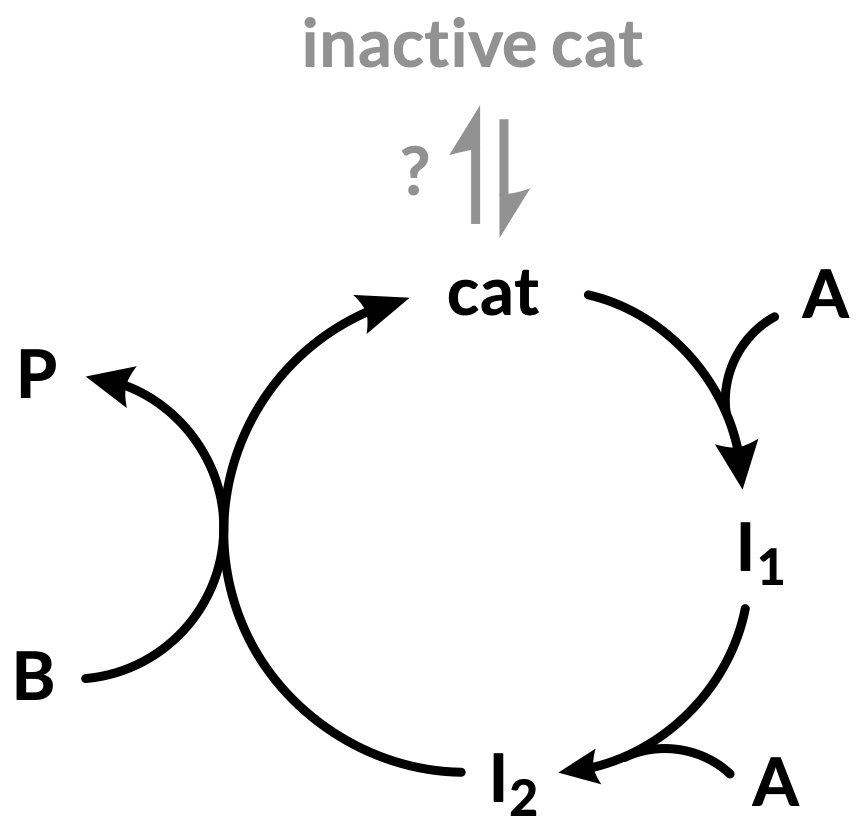
\includegraphics[width=5.4cm]{figures/CH3-cycle.png}
    \caption{A catalytic cycle with potential product inhibition.}
    \label{fig3-1:cycle}
\end{figure}

\keypoint{Reaction progress kinetic analysis (RPKA)} compares rates measured throughout complete reaction profiles.
Rate is plotted against a concentration that tracks reaction progress, so experiments are compared at matched compositions rather than matched times.

A \keypoint{same-excess experiment} is a new reaction started at substrate concentrations corresponding to a later point in the reference reaction.
The same-excess experiment therefore has the same substrate composition but a different reaction history: the catalyst is fresh and no product has yet accumulated unless it is added deliberately.

\solution{8.6cm}{%
  \centering

  \resizebox{\linewidth}{!}{%
    \begin{tikzpicture}[
        transform shape,
        axis/.style={draw=darkGrey,line width=1.5pt,->,>=Stealth},
        reference/.style={draw=paleRed,line width=3.2pt},
        same/.style={draw=paleBlue,line width=3.2pt},
        product/.style={draw=paleGreen,line width=3.2pt},
        datumref/.style={fill=darkRed,draw=darkRed,line width=0.5pt},
        datumsame/.style={fill=darkBlue,draw=darkBlue,line width=0.5pt},
        datumproduct/.style={fill=darkGreen,draw=darkGreen,line width=0.5pt},
        diagnostic/.style={draw=darkGrey,line width=1.7pt,->,>=Stealth},
        guide/.style={draw=darkGrey,dashed,line width=1.0pt},
        label/.style={font=\small\sffamily,text=darkGrey,align=center},
        title/.style={font=\sffamily,text=darkGrey,align=center}
      ]

      \path[use as bounding box] (0,-1.10) rectangle (17.3,7.75);

      % ==================================================
      % Product inhibition
      % ==================================================
      \node[title] at (4.15,7.28) {Product inhibition};
      \draw[axis] (0.8,1.0) -- (7.80,1.0);
      \draw[axis] (0.8,1.0) -- (0.8,6.70);
      \node[label,anchor=east] at (7.65,0.52) {$[\text{\textbf{A}}]$};
      \node[label,rotate=90] at (0.28,5.72) {rate};

      % Reference: r = 1.05 + 0.115([A]-1)^2
      \draw[reference]
        plot[domain=1.20:7.05,samples=100,variable=\x]
        (\x,{1.05 + 0.115*(\x - 1.00)^2});

      % Fresh same-excess: r = 1.55 + 0.155([A]-1)^2
      \draw[same]
        plot[domain=1.20:6.25,samples=100,variable=\x]
        (\x,{1.55 + 0.155*(\x - 1.00)^2});

      % Product-added reaction overlays the reference power law.
      \draw[product]
        plot[domain=1.20:7.05,samples=100,variable=\x]
        (\x,{1.05 + 0.115*(\x - 1.00)^2});

      % Filled circular data markers calculated from the same power laws.
      \foreach \x in {1.45,2.30,3.15,4.00,4.85,5.70,6.50,6.95} {
        \fill[datumref]
          (\x,{1.05 + 0.115*(\x - 1.00)^2}) circle (3.4pt);
      }
      \foreach \x in {1.55,2.40,3.25,4.10,4.95,5.70,6.15} {
        \fill[datumsame]
          (\x,{1.55 + 0.155*(\x - 1.00)^2}) circle (3.4pt);
      }
      \foreach \x in {1.65,2.50,3.35,4.20,5.05,5.90,6.60} {
        \fill[datumproduct]
          (\x,{1.05 + 0.115*(\x - 1.00)^2}) circle (3.4pt);
      }

      % Diagnostic arrow at one matched composition.
      \draw[guide] (4.45,1.0) -- (4.45,4.30);
      \draw[diagnostic]
        (4.45,{1.55 + 0.155*(4.45 - 1.00)^2})
        --
        (4.45,{1.05 + 0.115*(4.45 - 1.00)^2});
    %   \node[label,anchor=west] at (4.57,3.35)
    %     {$+\,\text{\textbf{P}}$};

      % Labels placed in unused upper-left area.
      \node[label,text=darkBlue,anchor=west] at (1.25,6.30)
        {same-excess with no product};
      \node[label,text=darkGreen,anchor=west] at (1.25,5.74)
        {$+\,\text{\textbf{P}}$: restores reference};

      % ==================================================
      % Catalyst deactivation
      % ==================================================
      \node[title] at (12.65,7.28) {Catalyst deactivation};
      \draw[axis] (9.30,1.0) -- (16.30,1.0);
      \draw[axis] (9.30,1.0) -- (9.30,6.70);
      \node[label,anchor=east] at (16.15,0.52) {$[\text{\textbf{A}}]$};
      \node[label,rotate=90] at (8.78,5.72) {rate};

      % Reference: lower power-law rate after catalyst ageing.
      \draw[reference]
        plot[domain=9.70:15.55,samples=100,variable=\x]
        (\x,{1.05 + 0.115*(\x - 9.50)^2});

      % Fresh same-excess: higher power-law rate.
      \draw[same]
        plot[domain=9.70:14.75,samples=100,variable=\x]
        (\x,{1.55 + 0.155*(\x - 9.50)^2});

      % Product addition leaves the fresh power-law profile unchanged.
      \draw[product]
        plot[domain=9.70:14.75,samples=100,variable=\x]
        (\x,{1.55 + 0.155*(\x - 9.50)^2});

      \foreach \x in {9.95,10.80,11.65,12.50,13.35,14.20,15.00,15.45} {
        \fill[datumref]
          (\x,{1.05 + 0.115*(\x - 9.50)^2}) circle (3.4pt);
      }
      \foreach \x in {10.05,10.90,11.75,12.60,13.45,14.20,14.65} {
        \fill[datumsame]
          (\x,{1.55 + 0.155*(\x - 9.50)^2}) circle (3.4pt);
      }
      \foreach \x in {10.15,11.00,11.85,12.70,13.55,14.30,14.70} {
        \fill[datumproduct]
          (\x,{1.55 + 0.155*(\x - 9.50)^2}) circle (3.4pt);
      }

      % Diagnostic arrow indicates loss of rate with catalyst history.
      \draw[guide] (12.95,1.0) -- (12.95,4.30);
      \draw[diagnostic]
        (12.95,{1.55 + 0.155*(12.95 - 9.50)^2})
        --
        (12.95,{1.05 + 0.115*(12.95 - 9.50)^2});

      % Labels placed in unused upper-left area.
      \node[label,text=darkGreen,anchor=west] at (9.75,6.30)
        {same-excess with more turnovers};
      \node[label,text=darkRed,anchor=west] at (9.75,5.74)
        {$+\,\text{\textbf{P}}$: no change};

      % ==================================================
      % Legend
      % ==================================================
      \draw[reference] (1.90,-0.12) -- (2.65,-0.12);
      \fill[datumref] (2.28,-0.12) circle (3.4pt);
      \node[label,anchor=west] at (2.82,-0.12) {reference};

      \draw[same] (6.15,-0.12) -- (6.90,-0.12);
      \fill[datumsame] (6.53,-0.12) circle (3.4pt);
      \node[label,anchor=west] at (7.07,-0.12) {same excess};

      \draw[product] (10.55,-0.12) -- (11.30,-0.12);
      \fill[datumproduct] (10.93,-0.12) circle (3.4pt);
      \node[label,anchor=west] at (11.47,-0.12)
        {same excess + product};

    \end{tikzpicture}%
  }
}

At the same substrate composition, the fresh same-excess reaction is faster than the reference reaction in both diagnostic examples.
For product inhibition, adding product to the fresh reaction lowers the rate onto the reference profile.
For catalyst deactivation, adding product has no effect; the reference profile is slower because the catalyst has experienced more turnovers.

\subsection{Different-excess experiments and reaction order}

Once catalyst deactivation and product inhibition have been assessed, reaction-progress profiles can be used to determine how individual components contribute to the observed rate law.
In a \keypoint{different-excess experiment}, the initial concentration of one component is changed so that its effect on rate can be isolated.

For a rate law of the form

\begin{equation}
  r = k_{\mathrm{obs}}
      [\text{\textbf{A}}]^{\alpha}
      [\text{\textbf{B}}]^{\beta}
      [\mathrm{cat}]^{\gamma},
\end{equation}

we can test a trial order in compound \textbf{B} by dividing the measured rate by $[\text{\textbf{B}}]^{\beta}$.
If the correct value of $\beta$ has been chosen, datasets collected using different excesses of compound \textbf{B} should collapse onto the same normalised relationship.

\solution{7.4cm}{%
  \centering

  \resizebox{\linewidth}{!}{%
    \begin{tikzpicture}[
        transform shape,
        axis/.style={draw=darkGrey,line width=1.5pt,->,>=Stealth},
        runone/.style={draw=paleBlue,line width=3.0pt},
        runtwo/.style={draw=paleRed,line width=3.0pt},
        datumone/.style={fill=darkBlue,draw=darkBlue},
        datumtwo/.style={fill=darkRed,draw=darkRed},
        guide/.style={draw=darkGrey,dashed,line width=1.0pt},
        label/.style={font=\small\sffamily,text=darkGrey,align=center},
        title/.style={font=\sffamily,text=darkGrey,align=center}
      ]

      \path[use as bounding box] (0,-0.45) rectangle (17.3,6.9);

      % ---------------------------------------------
      % Trial order is wrong
      % ---------------------------------------------
      \node[title] at (4.2,6.45) {Trial $\beta$ is incorrect};
      \draw[axis] (0.8,1.0) -- (7.8,1.0);
      \draw[axis] (0.8,1.0) -- (0.8,5.95);
      \node[label,anchor=east] at (7.65,0.52) {$[\text{\textbf{A}}]$};
      \node[label,rotate=90] at (0.25,4.90)
        {$\mathrm{rate} /[\text{\textbf{B}}]^{\beta}$};

      \draw[runone]
        plot[domain=1.25:7.0,samples=100,variable=\x]
        (\x,{1.05 + 0.105*(\x - 1.0)^2});
      \draw[runtwo]
        plot[domain=1.25:6.55,samples=100,variable=\x]
        (\x,{1.45 + 0.155*(\x - 1.0)^2});

      \foreach \x in {1.45,2.25,3.05,3.85,4.65,5.45,6.25,6.85} {
        \fill[datumone] (\x,{1.05 + 0.105*(\x - 1.0)^2}) circle (3.4pt);
      }
      \foreach \x in {1.55,2.35,3.15,3.95,4.75,5.55,6.35} {
        \fill[datumtwo] (\x,{1.45 + 0.155*(\x - 1.0)^2}) circle (3.4pt);
      }

      \node[label,text=darkBlue,anchor=west] at (1.2,5.45)
        {lower $[\text{\textbf{B}}]_0$};
      \node[label,text=darkRed,anchor=west] at (1.2,4.95)
        {higher $[\text{\textbf{B}}]_0$};

      % ---------------------------------------------
      % Correct trial order gives overlay
      % ---------------------------------------------
      \node[title] at (12.8,6.45) {Correct $\beta$: profiles overlay};
      \draw[axis] (9.4,1.0) -- (16.4,1.0);
      \draw[axis] (9.4,1.0) -- (9.4,5.95);
      \node[label,anchor=east] at (16.25,0.52) {$[\text{\textbf{A}}]$};
      \node[label,rotate=90] at (8.85,4.90)
        {$\mathrm{rate} /[\text{\textbf{B}}]^{\beta}$};

      \draw[runone]
        plot[domain=9.85:15.95,samples=100,variable=\x]
        (\x,{1.05 + 0.105*(\x - 9.6)^2});
      \draw[runtwo]
        plot[domain=9.85:15.95,samples=100,variable=\x]
        (\x,{1.05 + 0.105*(\x - 9.6)^2});

      \foreach \x in {10.05,10.85,11.65,12.45,13.25,14.05,14.85,15.65} {
        \fill[datumone] (\x,{1.05 + 0.105*(\x - 9.6)^2}) circle (3.4pt);
      }
      \foreach \x in {10.15,10.95,11.75,12.55,13.35,14.15,14.95,15.75} {
        \fill[datumtwo] (\x,{1.05 + 0.105*(\x - 9.6)^2}) circle (3.4pt);
      }

      \node[label,anchor=west] at (10.0,5.95)
        {normalisation removes the $[\text{\textbf{B}}]$ dependence};

    \end{tikzpicture}%
  }
}

The value of $\beta$ that gives the best overlay is the empirical order in compound \textbf{B} over the concentration range examined.
The same approach can be applied to other components of the reaction mixture.
Once the concentration dependences have been identified, the complete rate law can be tested directly.
Rearranging

\begin{equation}
  r = k_{\mathrm{obs}}
      [\text{\textbf{A}}]^{\alpha}
      [\text{\textbf{B}}]^{\beta}
      [\mathrm{cat}]^{\gamma}
\end{equation}

gives

\begin{equation}
  \frac{r}{[\text{\textbf{A}}]^{\alpha}[\mathrm{cat}]^{\gamma}}
  = k_{\mathrm{obs}}[\text{\textbf{B}}]^{\beta}.
\end{equation}

If the orders are correct, data from experiments performed with different initial concentrations should collapse onto the same straight line when plotted in this form.
The gradient is $k_{\mathrm{obs}}$.

\solution{6.5cm}{%
  \centering

  \resizebox{\linewidth}{!}{%
    \begin{tikzpicture}[
        transform shape,
        axis/.style={draw=darkGrey,line width=1.5pt,->,>=Stealth},
        fit/.style={draw=paleGreen,line width=3.2pt},
        datumone/.style={fill=darkBlue,draw=darkBlue},
        datumtwo/.style={fill=darkRed,draw=darkRed},
        datumthree/.style={fill=darkGreen,draw=darkGreen},
        slope/.style={draw=darkGrey,line width=1.3pt},
        label/.style={font=\small\sffamily,text=darkGrey,align=center}
      ]

      \path[use as bounding box] (0,-0.45) rectangle (17.3,6.2);

      \draw[axis] (1.4,0.9) -- (16.2,0.9);
      \draw[axis] (1.4,0.9) -- (1.4,5.55);

      \node[label,anchor=east] at (16.05,0.38)
        {$[\text{\textbf{B}}]^{\beta}$};
      \node[label,rotate=90] at (0.50,4.35)
        {$r/\left([\text{\textbf{A}}]^{\alpha}[\mathrm{cat}]^{\gamma}\right)$};

      % y = k_obs x
      \draw[fit] (2.1,1.15) -- (14.9,5.05);

      % Three experiments with different starting compositions collapse onto
      % the same linear relationship.
      \foreach \x/\y in {
        2.5/1.28,4.1/1.78,5.8/2.28,7.5/2.80,9.1/3.28
      } {
        \fill[datumone] (\x,\y) circle (3.6pt);
      }

      \foreach \x/\y in {
        3.0/1.43,4.8/1.98,6.5/2.50,8.2/3.01,10.0/3.56,11.6/4.04
      } {
        \fill[datumtwo] (\x,\y) circle (3.6pt);
      }

      \foreach \x/\y in {
        5.3/2.13,7.0/2.64,8.7/3.16,10.5/3.70,12.2/4.22,13.9/4.74
      } {
        \fill[datumthree] (\x,\y) circle (3.6pt);
      }

      % Slope annotation positioned away from the data.
      \draw[slope] (4.8,1.55) -- (6.8,1.55) -- (6.8,2.16);
      \node[label,anchor=west] at (7.05,1.84) {gradient $= k_{\mathrm{obs}}$};

      % Legend in unused upper-left region.
      \fill[datumone] (2.45,5.05) circle (3.6pt);
      \node[label,anchor=west] at (2.72,5.05) {experiment 1};

      \fill[datumtwo] (5.45,5.05) circle (3.6pt);
      \node[label,anchor=west] at (5.72,5.05) {experiment 2};

      \fill[datumthree] (8.45,5.05) circle (3.6pt);
      \node[label,anchor=west] at (8.72,5.05) {experiment 3};

    \end{tikzpicture}%
  }
}

A common straight line therefore provides a compact visual check that the proposed concentration dependences describe all of the reaction-progress datasets consistently.
Systematic curvature or separation between experiments indicates that the assumed rate law is incomplete.

\begin{conceptbox}
  \keypoint{Reaction order is empirical.}
  Values of $\alpha$, $\beta$, and $\gamma$ describe how the observed rate responds to concentration under the conditions examined.
  They constrain possible mechanisms, but should not automatically be interpreted as stoichiometric coefficients of an elementary step.
\end{conceptbox}

\subsection{Variable time normalisation analysis}

\keypoint{Variable time normalisation analysis (VTNA)} provides a graphical method for determining reaction orders directly from concentration--time profiles.\mcite{Bures2016}
VTNA compares the complete reaction profiles after transforming the time axis and hence is conceptually related to the reaction-progress methods introduced above.
However, it avoids differentiating concentration--time data to obtain instantaneous rates.

For a reaction with rate law

\begin{equation}
  r = k_{\mathrm{obs}}
      [\text{\textbf{A}}]^{\alpha}
      [\text{\textbf{B}}]^{\beta},
\end{equation}

we can determine the order in compound \textbf{A} by replacing time with the normalised time coordinate

  \begin{equation}
    t_{\mathrm{N},\alpha}
    = \int_0^t [\text{\textbf{A}}(\tau)]^{\alpha}\,\mathrm{d}\tau.
  \end{equation}

The value of $\alpha$ is varied until concentration profiles obtained from experiments with different initial concentrations of compound \textbf{A} overlay.
The value that gives the best overlay is the empirical order in compound \textbf{A}.

\solution{8.0cm}{%
  \centering

  \resizebox{\linewidth}{!}{%
    \begin{tikzpicture}[
        transform shape,
        axis/.style={draw=darkGrey,line width=1.5pt,->,>=Stealth},
        runone/.style={draw=paleBlue,line width=3.0pt},
        runtwo/.style={draw=paleRed,line width=3.0pt},
        datumone/.style={fill=darkBlue,draw=darkBlue},
        datumtwo/.style={fill=darkRed,draw=darkRed},
        arrow/.style={draw=darkGrey,line width=1.8pt,->,>=Stealth},
        label/.style={font=\small\sffamily,text=darkGrey,align=center},
        title/.style={font=\sffamily,text=darkGrey,align=center}
      ]

      \path[use as bounding box] (0,-0.5) rectangle (17.3,7.2);

      % ---------------------------------------------
      % Original concentration-time profiles
      % ---------------------------------------------
      \node[title] at (3.7,6.70) {Original reaction profiles};
      \draw[axis] (0.7,1.0) -- (6.7,1.0);
      \draw[axis] (0.7,1.0) -- (0.7,6.15);
      \node[label,anchor=east] at (6.55,0.52) {time, $t$};
      \node[label,rotate=90] at (0.18,5.15)
        {$[\text{\textbf{P}}]$};

      \draw[runone]
        plot[domain=1.05:6.10,samples=100,variable=\x]
        (\x,{1.15 + 4.40*(1 - exp(-0.44*(\x - 1.00)))});
      \draw[runtwo]
        plot[domain=1.05:5.55,samples=100,variable=\x]
        (\x,{1.15 + 4.40*(1 - exp(-0.72*(\x - 1.00)))});

      \foreach \x in {1.15,1.85,2.55,3.25,3.95,4.65,5.35,6.00} {
        \fill[datumone]
          (\x,{1.15 + 4.40*(1 - exp(-0.44*(\x - 1.00)))}) circle (3.4pt);
      }
      \foreach \x in {1.20,1.85,2.50,3.15,3.80,4.45,5.10,5.48} {
        \fill[datumtwo]
          (\x,{1.15 + 4.40*(1 - exp(-0.72*(\x - 1.00)))}) circle (3.4pt);
      }

      % Transformation arrow
      \draw[arrow] (7.15,3.65) -- (9.05,3.65);
      \node[label] at (8.10,4.15)
        {trial $\alpha$};

      % ---------------------------------------------
      % Normalised profiles
      % ---------------------------------------------
      \node[title] at (13.1,6.70) {Correct $\alpha$: profiles overlay};
      \draw[axis] (9.55,1.0) -- (16.45,1.0);
      \draw[axis] (9.55,1.0) -- (9.55,6.15);
      \node[label,anchor=east] at (16.30,0.52)
        {$t_{\mathrm{N},\alpha}$};
      \node[label,rotate=90] at (9.03,5.15)
        {$[\text{\textbf{P}}]$};

      \draw[runone]
        plot[domain=9.95:15.70,samples=100,variable=\x]
        (\x,{1.15 + 4.40*(1 - exp(-0.48*(\x - 9.85)))});
      \draw[runtwo]
        plot[domain=9.95:15.70,samples=100,variable=\x]
        (\x,{1.15 + 4.40*(1 - exp(-0.48*(\x - 9.85)))});

      \foreach \x in {10.05,10.85,11.65,12.45,13.25,14.05,14.85,15.55} {
        \fill[datumone]
          (\x,{1.15 + 4.40*(1 - exp(-0.48*(\x - 9.85)))}) circle (3.4pt);
      }
      \foreach \x in {10.20,11.00,11.80,12.60,13.40,14.20,15.00,15.62} {
        \fill[datumtwo]
          (\x,{1.15 + 4.40*(1 - exp(-0.48*(\x - 9.85)))}) circle (3.4pt);
      }

    \end{tikzpicture}%
  }
}

\begin{conceptbox}
  \keypoint{VTNA changes the time axis, not the measured concentration data.}
  The concentration profiles themselves are retained.
  The time coordinate is rescaled according to a trial concentration dependence, and the correct order is identified from the overlay of complete reaction profiles.
  This makes the method particularly useful for data-rich reaction monitoring.
\end{conceptbox}

\section{Linear free-energy relationships}

Linear free-energy relationships compare how structural changes influence the free energies of related reactions or equilibria.
They provide a familiar example of converting molecular structure into a numerical descriptor and relating that descriptor to an experimental response.

\subsection{The Hammett relationship}

The Hammett substituent constant, $\sigma_{\mathrm{X}}$, describes the electronic effect of substituent \textbf{X} relative to hydrogen.
The reaction constant, $\rho$, describes the sensitivity of a particular reaction to that substituent effect.

For a series of substituted reactions, the Hammett relationship is

\solution{3.3cm}{%
  \begin{equation}
    \log_{10}\left(\frac{k_{\mathrm{X}}}{k_{\mathrm{H}}}\right) = \rho\sigma_{\mathrm{X}}, \\
  \end{equation}
}

\solution{6.5cm}{%
  \centering

  \resizebox{\linewidth}{!}{%
    \begin{tikzpicture}[
        transform shape,
        axis/.style={draw=darkGrey,line width=1.5pt,->,>=Stealth},
        fit/.style={draw=paleRed,line width=3.2pt},
        datum/.style={fill=darkRed,draw=darkRed},
        guide/.style={draw=darkGrey,dashed,line width=1.0pt},
        slope/.style={draw=darkGrey,line width=1.3pt},
        label/.style={font=\small\sffamily,text=darkGrey,align=center}
      ]

      \path[use as bounding box] (0,-0.55) rectangle (17.3,6.75);

      % Axes cross at sigma = 0 and log(kX/kH) = 0.
      \draw[axis] (1.1,3.15) -- (16.2,3.15);
      \draw[axis] (8.35,0.75) -- (8.35,6.20);

      \node[label,anchor=east] at (16.05,2.68) {$\sigma_{\mathrm{X}}$};
      \node[label,rotate=90] at (7.72,5.18)
        {$\log_{10}(k_{\mathrm{X}}/k_{\mathrm{H}})$};

      % Positive Hammett relationship through the origin.
      \draw[fit] (2.1,1.15) -- (14.85,5.52);

      \foreach \x/\y in {
        2.75/1.37,
        4.10/1.84,
        5.55/2.33,
        6.95/2.80,
        8.35/3.15,
        9.75/3.62,
        11.15/4.12,
        12.55/4.58,
        14.05/5.10
      } {
        \fill[datum] (\x,\y) circle (3.6pt);
      }

      % Origin and substituent regions.
      \draw[guide] (8.35,3.15) -- (8.35,0.95);

      \node[label,anchor=north] at (3.85,4.30)
        {electron-donating\\substituents};
      \node[label,anchor=north] at (12.75,2.90)
        {electron-withdrawing\\substituents};

      % Slope marker near the early part of the relationship.
      \draw[slope]
        (4.55,1.55)
        -- (6.35,1.55)
        -- (6.35,2.17);
      \node[label,anchor=west] at (4.2,1.2)
        {gradient $=\rho$};

    \end{tikzpicture}%
  }
}

A positive value of $\rho$ means that electron-withdrawing substituents increase the measured rate relative to the reaction with hydrogen.
A negative value means that electron-donating substituents increase the measured rate.
The magnitude of $\rho$ describes how strongly the reaction responds to the substituent series.

In the language introduced earlier, each substituted reaction is an \keypoint{observation}, $\sigma_{\mathrm{X}}$ is a \keypoint{descriptor} (or a \keypoint{feature}), $\log_{10}(k_{\mathrm{X}}/k_{\mathrm{H}})$ is the \keypoint{target}, and $\rho$ is the fitted \keypoint{coefficient} of a linear model.

\section{Deviation from linearity}

Systematic curvature, a break in slope, or a distinct group of outliers indicates that the simple one-parameter model is incomplete.
Possible explanations include a change in mechanism, a change in the turnover- or rate-determining transition state, or a substituent effect that is not captured adequately by the chosen $\sigma$ values.

\solution{6.5cm}{%
  \centering

  \resizebox{\linewidth}{!}{%
    \begin{tikzpicture}[
        transform shape,
        axis/.style={draw=darkGrey,line width=1.5pt,->,>=Stealth},
        curve/.style={draw=paleBlue,line width=3.0pt},
        lineone/.style={draw=paleRed,line width=3.0pt},
        linetwo/.style={draw=paleGreen,line width=3.0pt},
        datumblue/.style={fill=darkBlue,draw=darkBlue},
        datumred/.style={fill=darkRed,draw=darkRed},
        datumgreen/.style={fill=darkGreen,draw=darkGreen},
        guide/.style={draw=darkGrey,dashed,line width=1.0pt},
        label/.style={font=\small\sffamily,text=darkGrey,align=center},
        title/.style={font=\sffamily,text=darkGrey,align=center}
      ]

      \path[use as bounding box] (0,-0.55) rectangle (17.3,6.95);

      % ==================================================
      % Curvature
      % ==================================================
      \node[title] at (4.15,6.50) {Curvature};
      \draw[axis] (0.8,1.0) -- (7.75,1.0);
      \draw[axis] (0.8,1.0) -- (0.8,5.95);
      \node[label,anchor=east] at (7.60,0.52) {$\sigma_{\mathrm{X}}$};
      \node[label,rotate=90] at (0.25,5.00)
        {$\log_{10}(k_{\mathrm{X}}/k_{\mathrm{H}})$};

      \draw[curve]
        plot[domain=1.25:7.05,samples=100,variable=\x]
        (\x,{1.18 + 0.115*(\x - 1.05)^2});

      \foreach \x in {1.45,2.20,2.95,3.70,4.45,5.20,5.95,6.70} {
        \fill[datumblue]
          (\x,{1.18 + 0.115*(\x - 1.05)^2}) circle (3.5pt);
      }

      \node[label,anchor=west] at (1.5,6)
        {one straight line is inadequate};

      % ==================================================
      % Break in slope
      % ==================================================
      \node[title] at (12.70,6.50) {Break in slope};
      \draw[axis] (9.30,1.0) -- (16.25,1.0);
      \draw[axis] (9.30,1.0) -- (9.30,5.95);
      \node[label,anchor=east] at (16.10,0.52) {$\sigma_{\mathrm{X}}$};
      \node[label,rotate=90] at (8.75,5.00)
        {$\log_{10}(k_{\mathrm{X}}/k_{\mathrm{H}})$};

      % Two distinct linear regimes joined at the breakpoint.
      \draw[lineone] (9.85,1.35) -- (12.65,2.70);
      \draw[linetwo] (12.65,2.70) -- (15.75,5.45);

      \foreach \x/\y in {
        10.15/1.50,
        10.80/1.81,
        11.45/2.12,
        12.10/2.44
      } {
        \fill[datumred] (\x,\y) circle (3.5pt);
      }

      \foreach \x/\y in {
        12.80/2.84,
        13.45/3.42,
        14.10/4.00,
        14.75/4.57,
        15.40/5.15
      } {
        \fill[datumgreen] (\x,\y) circle (3.5pt);
      }

      \draw[guide] (12.65,1.0) -- (12.65,2.70);
      \node[label,anchor=west] at (12.82,1.60)
        {change in response};

    \end{tikzpicture}%
  }
}

The important question is not simply whether the correlation has a high $R^2$ value.
The pattern of the deviations should be inspected and interpreted chemically.
A failed linear relationship can therefore reveal behaviour that would be hidden by reporting only the fitted slope.

\subsection{Non-linear effects in catalysis}

  Departure from a simple linear relationship is not unique to LFERs.
  In asymmetric catalysis, a simple expectation is that the enantiomeric excess of the product changes linearly with the enantiomeric excess of the chiral catalyst.
  A deviation from this relationship is called a \keypoint{nonlinear effect (NLE)}.\mcite{Kagan1986}

  \solution{5.7cm}{%
    \centering

    \resizebox{\linewidth}{!}{%
      \begin{tikzpicture}[
          transform shape,
          axis/.style={draw=darkGrey,line width=1.5pt,->,>=Stealth},
          ideal/.style={draw=paleBlue,line width=3.0pt},
          positive/.style={draw=paleRed,line width=3.0pt},
          negative/.style={draw=paleGreen,line width=3.0pt},
          datumideal/.style={fill=darkBlue,draw=darkBlue},
          datumpositive/.style={fill=darkRed,draw=darkRed},
          datumnegative/.style={fill=darkGreen,draw=darkGreen},
          label/.style={font=\small\sffamily,text=darkGrey,align=center}
        ]

        \path[use as bounding box] (0,-0.45) rectangle (17.3,6.2);

        \draw[axis] (1.25,0.9) -- (16.1,0.9);
        \draw[axis] (1.25,0.9) -- (1.25,5.65);

        \node[label,anchor=east] at (15.95,0.38)
          {$ee_{\mathrm{catalyst}}$};
        \node[label,rotate=90] at (0.55,4.55)
          {$ee_{\mathrm{product}}$};

        % Linear expectation.
        \draw[ideal] (2.0,1.15) -- (14.85,5.10);

        % Positive NLE: product ee is amplified above the linear expectation.
        \draw[positive]
          plot[domain=2.0:14.85,samples=100,variable=\x]
          (\x,{1.15 + 3.95*sqrt((\x - 2.0)/(14.85 - 2.0))});

        % Negative NLE: product ee falls below the linear expectation.
        \draw[negative]
          plot[domain=2.0:14.85,samples=100,variable=\x]
          (\x,{1.15 + 3.95*((\x - 2.0)/(14.85 - 2.0))^2});

        \foreach \x/\y in {
          3.25/1.53,5.40/2.19,7.55/2.85,9.70/3.51,11.85/4.17,14.00/4.84
        } {
          \fill[datumideal] (\x,\y) circle (3.5pt);
        }

        \foreach \x in {3.25,5.40,7.55,9.70,11.85,14.00} {
          \fill[datumpositive]
            (\x,{1.15 + 3.95*sqrt((\x - 2.0)/(14.85 - 2.0))}) circle (3.5pt);
          \fill[datumnegative]
            (\x,{1.15 + 3.95*((\x - 2.0)/(14.85 - 2.0))^2}) circle (3.5pt);
        }

        \node[label,text=darkRed,anchor=west] at (10.75,5.28)
          {positive NLE};
        \node[label,text=darkBlue,anchor=west] at (11.15,3.68)
          {linear expectation};
        \node[label,text=darkGreen,anchor=west] at (10.55,2.05)
          {negative NLE};

      \end{tikzpicture}%
    }
  }

  Nonlinear behaviour can arise when the composition or aggregation state of the catalytically relevant species changes with catalyst enantiomeric composition.
  The shape of the relationship can therefore contain mechanistic information that would be lost by considering only a single selectivity measurement.

  The 2026 Nobel Prize in Chemistry recognised Henri Kagan and Kenso Soai for the discovery of nonlinear effects and autocatalysis in asymmetric organic synthesis.
  The Soai reaction provides an extreme example in which the reaction product participates in catalysing its own formation and small initial asymmetries can be amplified.\mcite{Soai1995}
  The detailed chemistry is beyond the scope of this course; the important point here is that \keypoint{departure from the simple model can itself be chemically informative}.

  \subsection{Separating electronic and steric effects}

The Hammett equation describes substituent effects using a single electronic parameter, $\sigma$.
For many reactions, however, changing a substituent alters more than its electronic influence: steric demand and other molecular properties can also affect the measured response.
A useful extension is therefore to describe the reaction using more than one physically meaningful parameter.

The Taft approach separates polar and steric contributions using independent substituent parameters.\mcite{Taft1952}
Schematically, a two-parameter linear free-energy relationship can be written as

\solution{2.8cm}{%
  \begin{equation}
    \log_{10}\left(\frac{k_{\mathrm{X}}}{k_{\mathrm{H}}}\right)
      = \rho\sigma_{\mathrm{X}} + \delta E_{\mathrm{s},\mathrm{X}},
  \end{equation}
}

where $E_{\mathrm{s},\mathrm{X}}$ describes the steric effect associated with substituent \textbf{X}, while $\rho$ and $\delta$ describe the sensitivity of the reaction to the electronic and steric terms, respectively.
The precise definition of a descriptor depends on the relationship being used; the important point is that different numerical parameters can encode different chemical effects.

\solution{7.2cm}{%
  \centering

  \resizebox{\linewidth}{!}{%
    \begin{tikzpicture}[
        transform shape,
        axis/.style={draw=darkGrey,line width=1.5pt,->,>=Stealth},
        electronic/.style={draw=paleRed,line width=3.0pt},
        steric/.style={draw=paleBlue,line width=3.0pt},
        combined/.style={draw=paleGreen,line width=3.0pt},
        datume/.style={fill=darkRed,draw=darkRed},
        datums/.style={fill=darkBlue,draw=darkBlue},
        datumc/.style={fill=darkGreen,draw=darkGreen},
        arrow/.style={draw=darkGrey,line width=1.8pt,->,>=Stealth},
        label/.style={font=\small\sffamily,text=darkGrey,align=center},
        title/.style={font=\sffamily,text=darkGrey,align=center}
      ]

      \path[use as bounding box] (0,-0.45) rectangle (17.3,6.8);

      % One electronic descriptor
      \node[title] at (3.45,6.30) {Electronic effect only};
      \draw[axis] (0.7,1.0) -- (6.2,1.0);
      \draw[axis] (0.7,1.0) -- (0.7,5.75);
      \node[label,anchor=east] at (6.05,0.52) {$\sigma_{\mathrm{X}}$};

      \draw[electronic] (1.25,1.45) -- (5.55,4.75);
      \foreach \x/\y in {
        1.45/1.58,
        2.10/2.05,
        2.75/2.82,
        3.40/2.96,
        4.05/3.95,
        4.70/4.05,
        5.35/4.90
      } {
        \fill[datume] (\x,\y) circle (3.5pt);
      }
      \node[label,anchor=west] at (1.8,5.75)
        {systematic residuals};

      % Arrow to multidimensional description
      \draw[arrow] (6.65,3.35) -- (8.35,3.35);
      \node[label] at (7.50,4.1)
        {add steric\\information};

      % Two descriptors conceptualised as a response surface / plane
      \node[title] at (12.60,6.30) {Electronic + steric effects};

      \draw[axis] (9.25,1.15) -- (15.85,1.15);
      \draw[axis] (9.25,1.15) -- (9.25,5.65);
      \draw[axis] (9.25,1.15) -- (11.20,0.35);

      \node[label,anchor=east] at (15.75,0.70) {$\sigma_{\mathrm{X}}$};
      \node[label,anchor=north] at (11.25,0.28) {$E_{\mathrm{s},\mathrm{X}}$};

      % Schematic fitted plane using simple projected edges.
      \fill[paleGreen,opacity=0.55]
        (10.15,1.80) -- (14.55,2.55) -- (15.45,4.65) -- (11.05,3.90) -- cycle;
      \draw[combined]
        (10.15,1.80) -- (14.55,2.55) -- (15.45,4.65) -- (11.05,3.90) -- cycle;

      \foreach \x/\y in {
        10.65/2.05,
        11.55/2.45,
        12.40/2.58,
        13.20/3.05,
        14.05/3.35,
        14.75/4.05,
        12.30/3.25,
        13.55/3.72
      } {
        \fill[datumc] (\x,\y) circle (3.5pt);
      }

      \node[label,anchor=west] at (10.6,5.75)
        {described simultaneously};

    \end{tikzpicture}%
  }
}

Adding descriptors can improve a quantitative relationship, but each additional term should still have a chemical interpretation.
Electronic and steric parameters are therefore an early example of \keypoint{multivariate molecular description}: one molecule is represented by several numerical features rather than by a single substituent constant.
This idea will become central when we move from classical physical-organic parameters to modern molecular descriptors and chemical space.

% !TeX root = ../notes.tex

\chapter{Exploring chemical space}

\begin{notebox}
  \keypoint{What do you need to learn from this chapter?}
  This chapter examines how molecular structure can be represented using numerical descriptors and how collections of molecules can be compared within multidimensional chemical spaces.
  You should understand that descriptor choice determines which molecular differences are represented, how similarity and distance depend on that representation, and why dimensionality reduction is required to visualise high-dimensional data.
  Particular emphasis is placed on connecting classical physical-organic parameters with modern molecular descriptors and on interpreting chemical-space maps critically.
\end{notebox}

\section{From physical-organic parameters to molecular descriptors}

The previous chapter used numerical parameters to describe how changes in molecular structure influence chemical behaviour.
Hammett substituent constants encode electronic effects, while Taft-type relationships introduce an additional steric contribution.
These parameters are examples of \keypoint{molecular descriptors}: numerical quantities used to describe molecular structure or properties.
A descriptor does not reproduce the complete molecule, but selects aspects of the molecule that may be relevant to the chemical question being asked.

\solution{4.0cm}{%
  \centering
  \begin{tabular}{@{}ll@{}}
    \textbf{Hammett:} & molecule $\longrightarrow \sigma_{\mathrm{X}}$ \\[0.55em]
    \textbf{Taft:} & molecule $\longrightarrow \left(\sigma_{\mathrm{X}},E_{\mathrm{s},\mathrm{X}}\right)$ \\[0.55em]
    \textbf{Modern:} & molecule $\longrightarrow \mathbf{x}=\left(x_1,x_2,\ldots,x_p\right)$
  \end{tabular}
}

The descriptor vector $\mathbf{x}$ may contain experimental measurements, calculated molecular properties, or values derived directly from molecular structure.
Examples include molecular mass, polarity, orbital energies, atomic charges, steric dimensions, and counts of structural fragments.

\solution{10.0cm}{%
  \centering

  \begin{tikzpicture}[
      transform shape,
      term/.style={
        draw=darkBlue,
        fill=paleBlue,
        line width=2.0pt,
        minimum width=8.0cm,
        minimum height=1.0cm,
        align=center,
        font=\sffamily
      },
      arrow/.style={
        ->,
        >=Stealth,
        draw=darkGrey,
        line width=2.3pt
      }
    ]

    \node[term] (structure) at (0,3.6)
      {molecular structure};

    \node[term] (descriptors) at (0,1.8)
      {descriptor vector $\mathbf{x}=(x_1,x_2,\ldots,x_p)$};

    \node[term] (space) at (0,0)
      {a point in multidimensional chemical space};

    \draw[arrow] (structure) -- (descriptors);
    \draw[arrow] (descriptors) -- (space);

  \end{tikzpicture}
  \\[1em]
  \begin{equation}
    \mathbf{X}
    =
    \begin{bmatrix}
      x_{11} & x_{12} & \cdots & x_{1p} \\
      x_{21} & x_{22} & \cdots & x_{2p} \\
      \vdots & \vdots & \ddots & \vdots \\
      x_{n1} & x_{n2} & \cdots & x_{np}
    \end{bmatrix},
  \end{equation}
}

\begin{conceptbox}
  \keypoint{A molecular descriptor is a selective representation.}
  Descriptors make modelling possible by converting chemical structure into numerical vectors.
  Their usefulness depends on whether the encoded information is relevant to the chemical question.
  The same molecule can occupy different positions in the chemical space when described by a different set of descriptors.
\end{conceptbox}

\subsection{A modern descriptor library: kraken}

The simple descriptor vector introduced above can contain many different kinds of chemical information.
The \textit{kraken} library provides a useful example for organophosphorus ligands used in homogeneous catalysis.\mcite{Gensch2022}
Rather than describing each ligand using a single electronic or steric parameter, the library combines many calculated physicochemical descriptors, which include quantities describing electronic structure, molecular geometry, and intermolecular interactions (Fig.~\ref{fig4-1:kraken}).

\begin{figure}[h!]
    \centering
    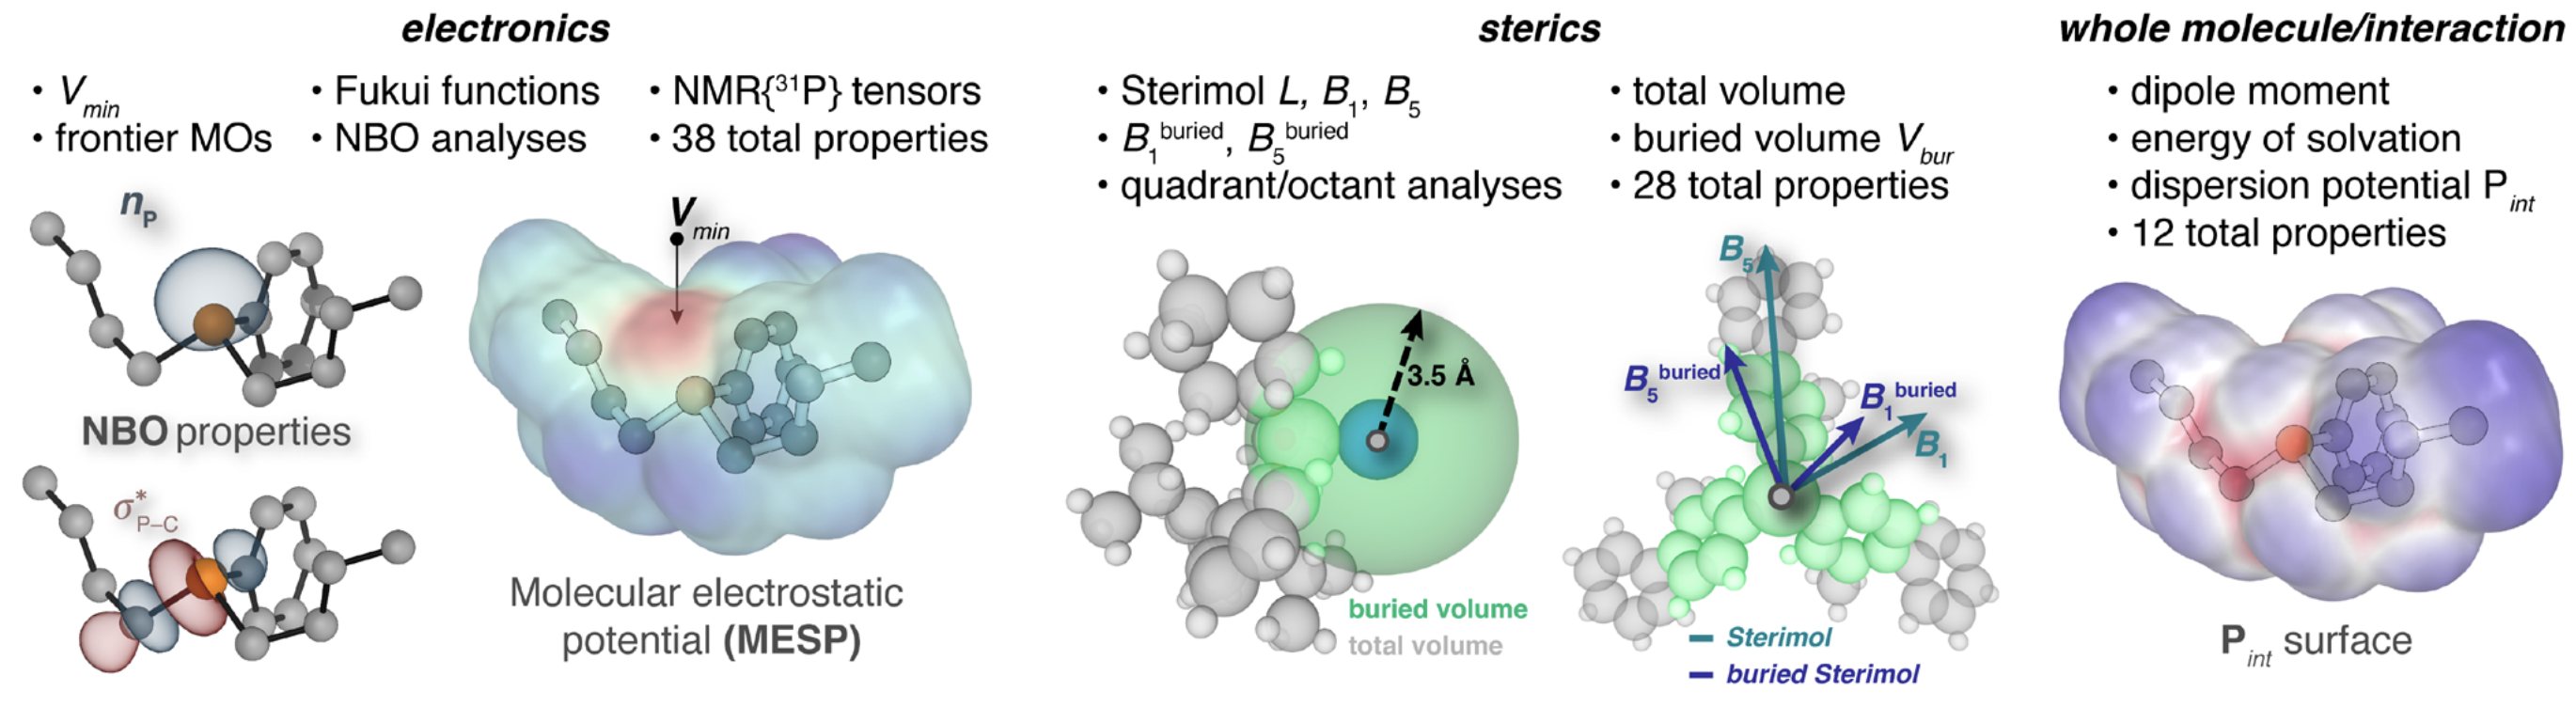
\includegraphics[width=\textwidth]{figures/CH4-kraken.png}
    \caption{Example physical organic descriptors in the \textit{kraken} library.}
    \label{fig4-1:kraken}
\end{figure}

\begin{warningbox}
Many molecular descriptors depend on three-dimensional structure.
For a flexible molecule, however, there is not one unique molecular geometry: several conformers may be accessible under the conditions of interest.
Properties can then be condensed across the ensemble in several ways, including their minimum, maximum, range, or a Boltzmann-weighted average.
\end{warningbox}

Steric effects were initially described using single numerical parameters (Fig.~\ref{fig4-2:steric-descriptor-progression}).
Examples include A-values, interference values, and the Taft steric parameter, $E_{\mathrm{s}}$.\mcite{Winstein1955,Taft1952}
These values provide useful relative measures of steric demand, but compress a three-dimensional molecular shape into one number.

\begin{figure}[htbp]
  \centering
  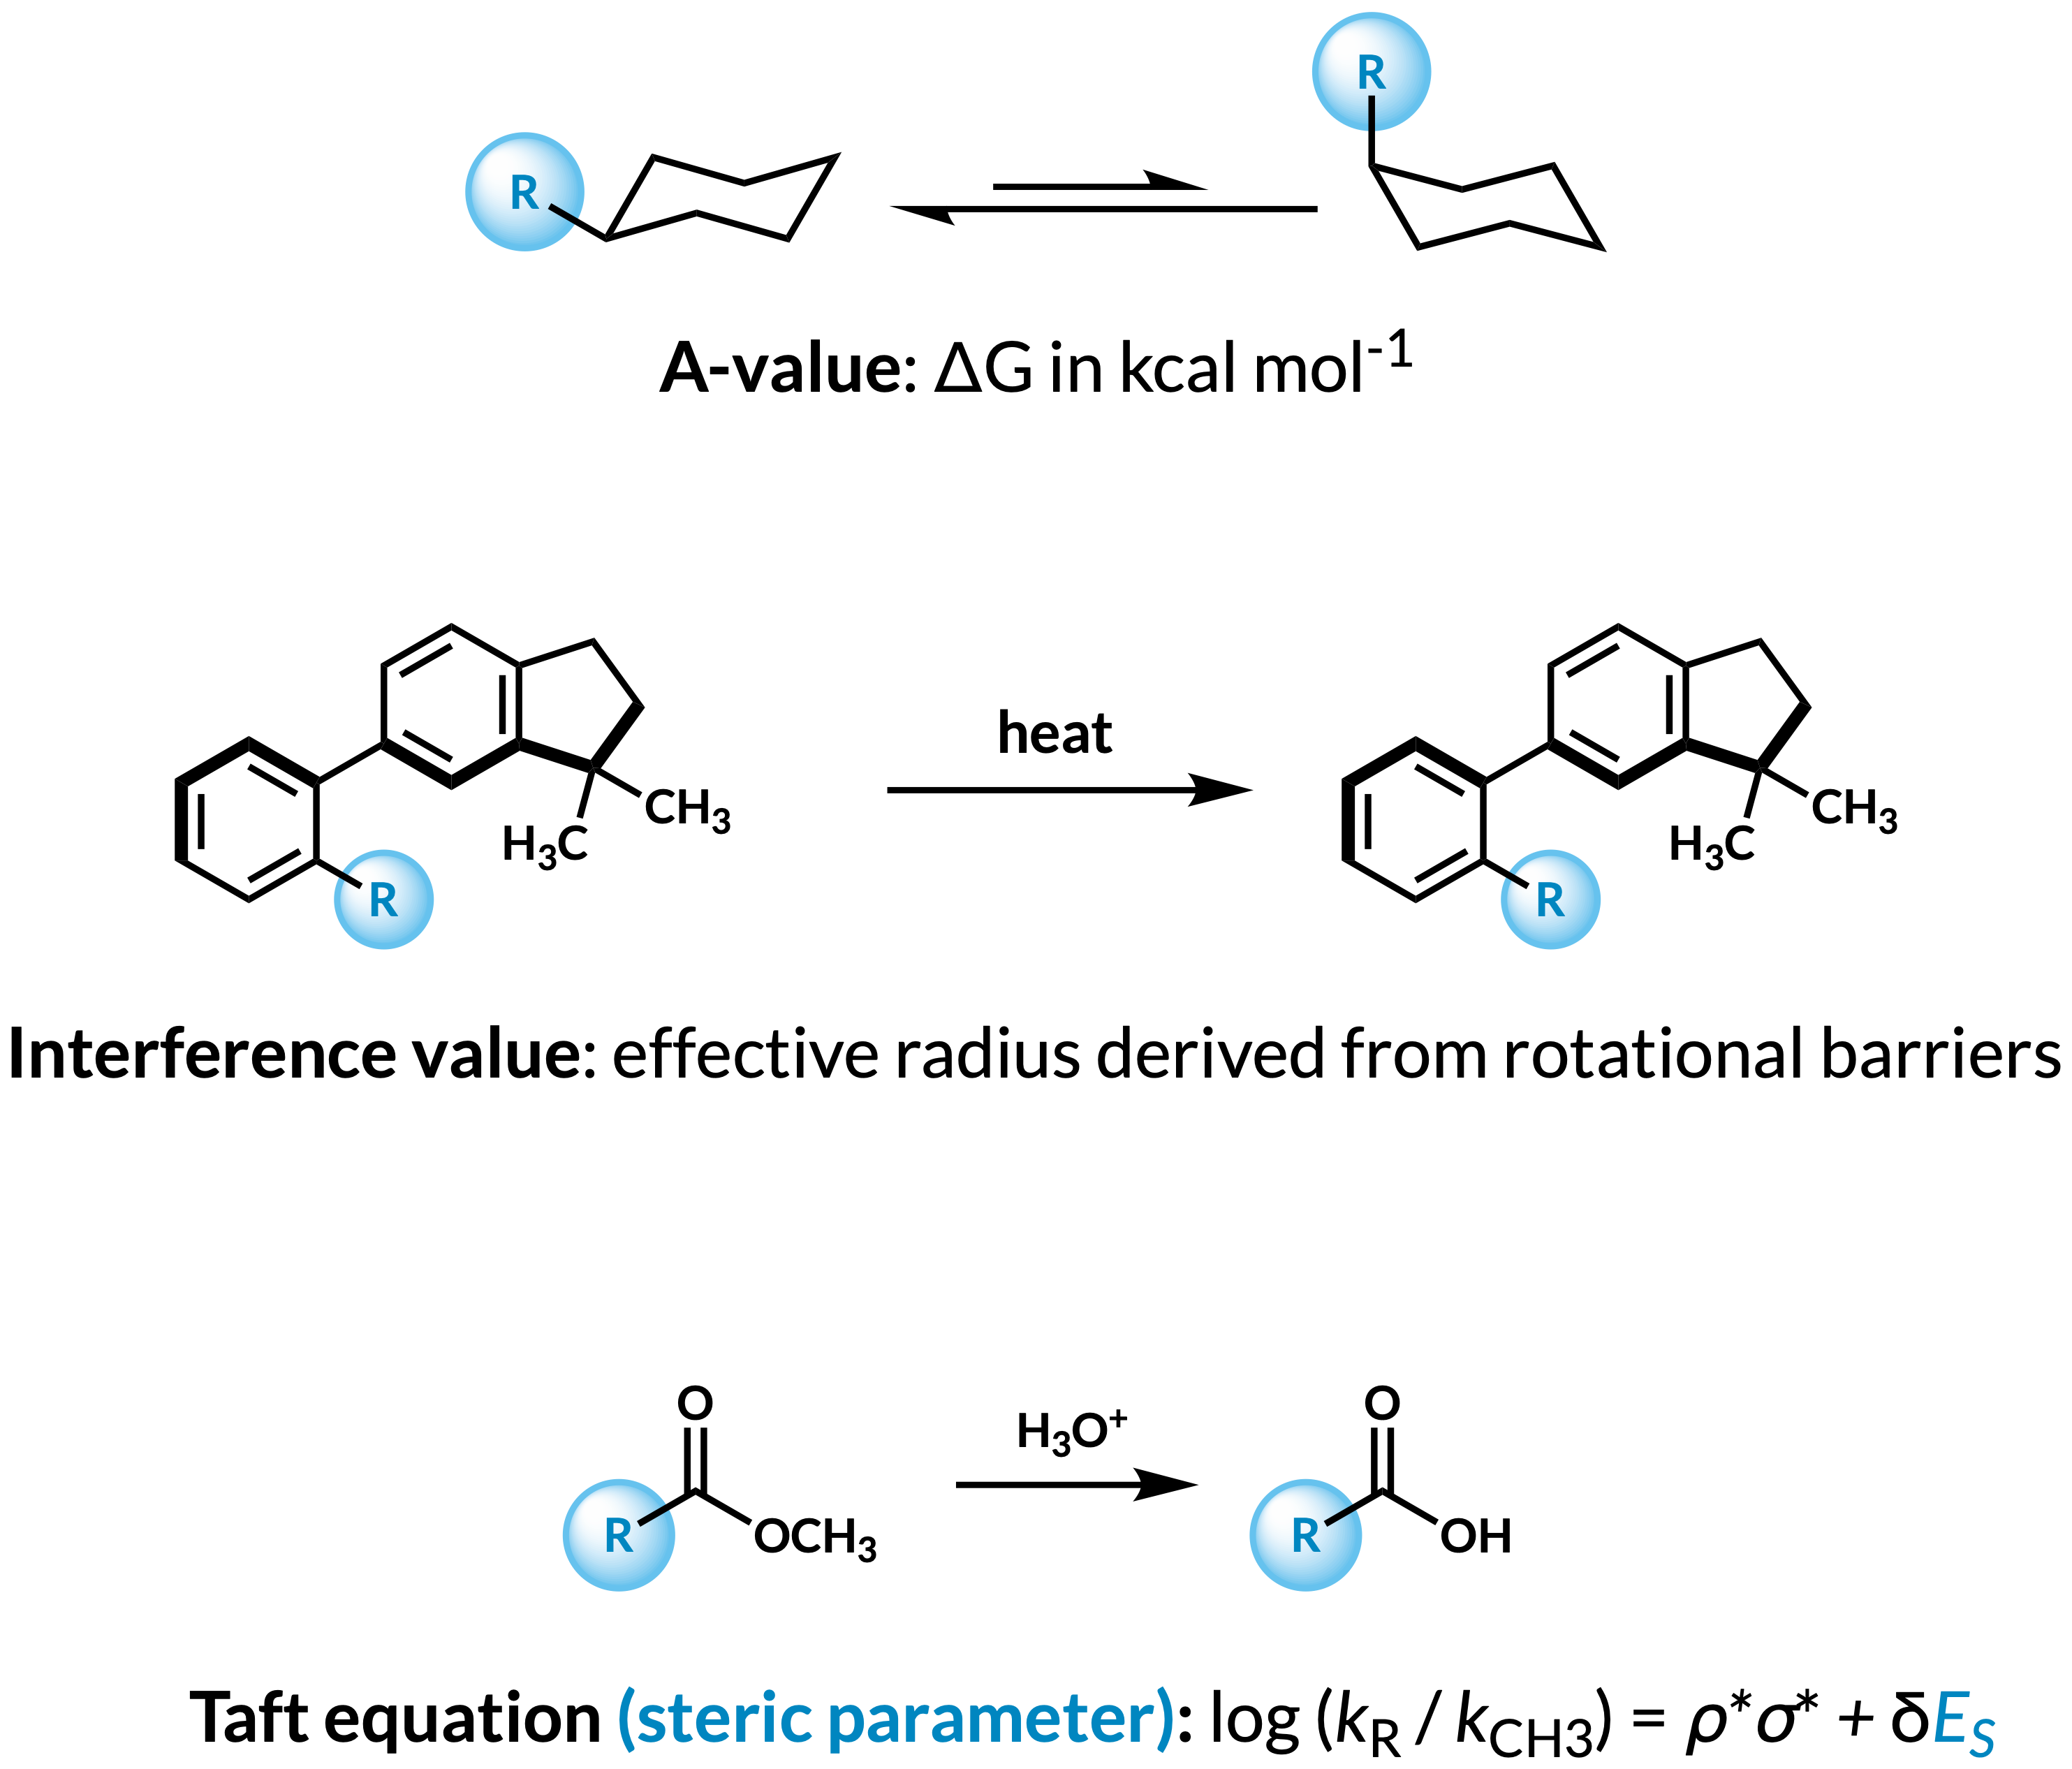
\includegraphics[width=0.75\linewidth]{figures/CH4-steric-descriptors.png}
  \caption{
    Evolution of steric descriptors from scalar parameters to directional descriptions.
    Scalar parameters such as A-values and $E_{\mathrm{s}}$ summarise steric demand using one value. 
    }
  \label{fig4-2:steric-descriptor-progression}
\end{figure}

More detailed descriptors retain information about the direction and spatial distribution of steric demand.
The Sterimol parameters are defined relative to a chosen primary axis, commonly the bond connecting a substituent to the molecular framework.\mcite{Brethome2019}
The parameter $L$ describes extension along this axis, while $B_1$ and $B_5$ describe the minimum and maximum widths perpendicular to it (Fig.~\ref{fig4-3:sterimol}).
This directional description is particularly useful for nonsymmetrical substituents that cannot be represented adequately by a single steric constant.

\begin{figure}[htbp]
  \centering
  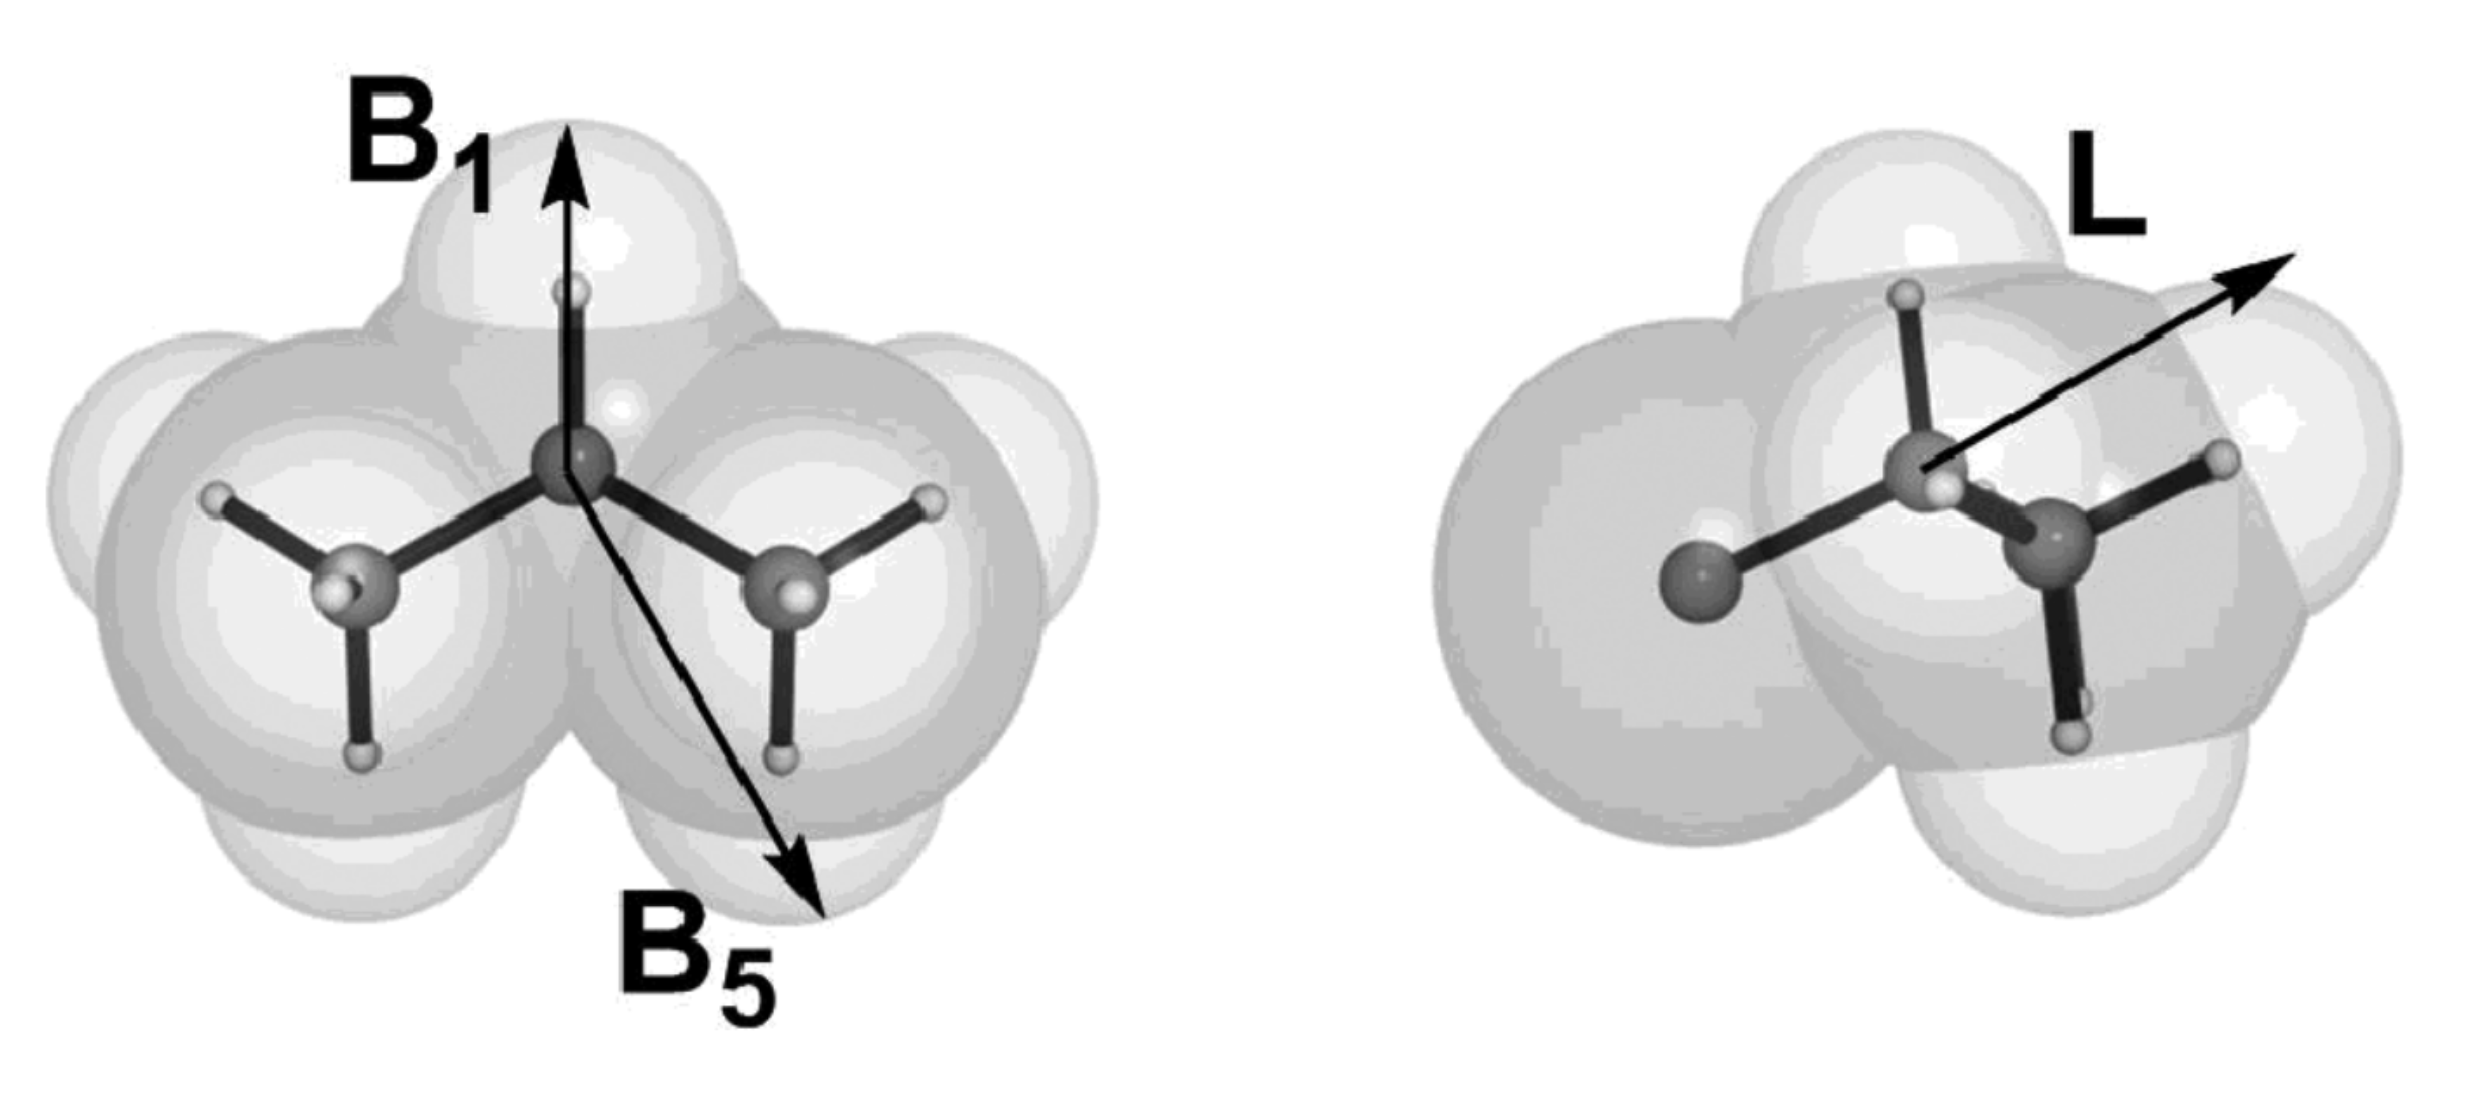
\includegraphics[width=0.75\linewidth]{figures/CH4-sterimol.png}
  \caption{Sterimol parameters. The parameter $L$ describes extension along this axis, while $B_1$ and $B_5$ describe the minimum and maximum widths perpendicular to it.}
  \label{fig4-3:sterimol}
\end{figure}

\solution{4cm}{%
  \textbf{A useful descriptor should be:}
  \begin{itemize}
    \item invariant;
    \item discriminating;
    \item chemically relevant;
    \item no more complex than required.
  \end{itemize}
}

\section{Comparing molecules}

Once molecules have been represented using a common set of descriptors, their similarity can be expressed quantitatively.
The simplest approach is to treat each descriptor as an axis and compare the positions of two molecules in the resulting descriptor space. For continuous descriptors, a common measure is the \keypoint{Euclidean distance} between two descriptor vectors.

\solution{6.5cm}{%
  \centering

  molecule \textbf{A} $\longrightarrow \mathbf{x}_{\mathrm{A}}$
  \qquad
  molecule \textbf{B} $\longrightarrow \mathbf{x}_{\mathrm{B}}$

  \vspace{0.9em}

  molecular comparison
  $\longrightarrow$
  distance between $\mathbf{x}_{\mathrm{A}}$ and $\mathbf{x}_{\mathrm{B}}$
  
    \vspace{0.9em}

  \begin{equation}
    d_{\mathrm{AB}}
    =
    \left[
      \sum_{j=1}^{p}
      \left(x_{\mathrm{A}j}-x_{\mathrm{B}j}\right)^2
    \right]^{1/2}.
  \end{equation}
}

\subsection{Descriptor scaling}

Descriptor values can have very different numerical ranges and physical units.
For example, molecular mass may vary by hundreds of daltons, while an orbital energy may vary by only a few electronvolts and a buried-volume descriptor may be expressed as a percentage.
Without scaling, descriptors with the largest numerical variation can dominate a distance calculation.

A common transformation is therefore to centre and scale each descriptor,

  \begin{equation}
    z_{ij}
    =
    \frac{x_{ij}-\bar{x}_j}{s_j},
  \end{equation}

where $\bar{x}_j$ and $s_j$ are the mean and standard deviation of descriptor $j$ within the dataset.
After standardisation, each descriptor is expressed relative to its variation within that dataset rather than in its original physical units.
Hence, all descriptors contribute comparably to the final distance.

\subsection{Similarity between fingerprints}

The molecular fingerprints introduced previously are binary representations rather than collections of continuous physicochemical descriptors.
For binary fingerprints, similarity is commonly measured using the \keypoint{Tanimoto coefficient}.\mcite{Bajusz2015}
If fingerprint \textbf{A} contains $a$ active bits, fingerprint \textbf{B} contains $b$ active bits, and $c$ bits are active in both fingerprints, then

\solution{3.0cm}{%
  \begin{equation}
    T_{\mathrm{AB}}
    =
    \frac{c}{a+b-c}.
  \end{equation}
}

The Tanimoto coefficient ranges from zero for fingerprints with no shared active bits to one for identical fingerprints.
It therefore measures similarity according to the structural features encoded by that particular fingerprint.

For a collection of molecules, similarities can be calculated between every unique pair of fingerprints.
For $N$ molecules, the number of pairwise comparisons is

  \begin{equation}
    N_{\mathrm{pairs}}
    =
    \frac{N(N-1)}{2}.
  \end{equation}

For example, a collection of 100 molecules contains 4950 unique molecular pairs.
The complete set of pairwise similarities can be arranged as a symmetric similarity matrix,

  \begin{equation}
    \mathbf{T}
    =
    \begin{bmatrix}
      1 & T_{12} & T_{13} & \cdots & T_{1N} \\
      T_{21} & 1 & T_{23} & \cdots & T_{2N} \\
      T_{31} & T_{32} & 1 & \cdots & T_{3N} \\
      \vdots & \vdots & \vdots & \ddots & \vdots \\
      T_{N1} & T_{N2} & T_{N3} & \cdots & 1
    \end{bmatrix}.
  \end{equation}

The matrix is symmetric because $T_{ij}=T_{ji}$, and every diagonal element is one because each molecule is identical to itself.
If the objective is only to find molecules similar to one query structure, the query fingerprint instead needs to be compared only with the other molecules in the collection.

\begin{conceptbox}
  \keypoint{Molecular similarity is representation dependent.} Euclidean distance compares molecules according to continuous descriptors, while the Tanimoto coefficient compares the features encoded in a molecular fingerprint.
  Two molecules can appear similar in one representation and not in another.
\end{conceptbox}

\solution{3.6cm}{%
  \centering

  \textbf{molecular similarity}
  $=$ \\[0.4em]
  \textbf{representation} \\[0.4em]
  $+$ 
  \textbf{preprocessing} \\[0.4em]
  $+$ 
  \textbf{comparison metric}
}

Once a common representation and metric have been chosen, the collection of molecular positions defines a \keypoint{chemical space} that can be explored for similarities, differences, gaps, and regions of interest.

\section{Mapping chemical spaces}

Chemical space becomes most useful when its axes correspond to chemically meaningful properties.
Ligand design provides an early example because both electronic donation and steric demand can influence the behaviour of a metal catalyst.
Tolman's work on monodentate phosphorus ligands provides a particularly useful historical example.\mcite{Tolman1977}
Electronic effects can be described using the Tolman electronic parameter, while steric demand can be described using the Tolman cone angle.
Plotting the two parameters against one another converts a list of ligand properties into a two-dimensional ligand space (Fig.~\ref{fig4-4:tolman-ligand-space})
A ligand-selection problem can therefore be reframed from choosing familiar structures to choosing molecules that sample distinct regions of property space.

\begin{figure}[htbp]
  \centering
  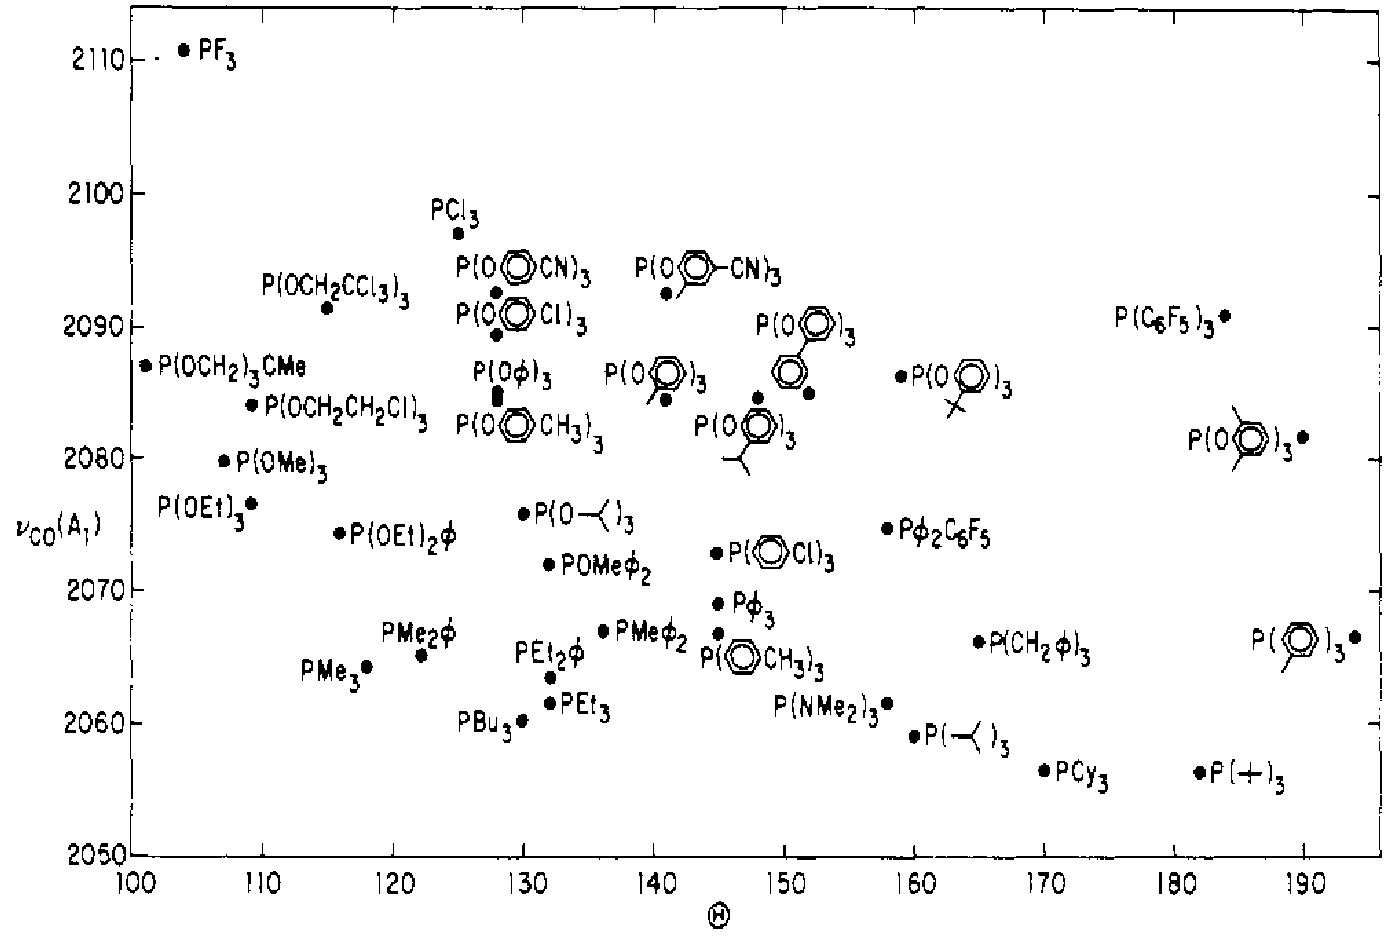
\includegraphics[width=0.82\linewidth]{figures/CH4-tolman.png}
  \caption{
    Steric--electronic ligand space constructed using Tolman's electronic and steric parameters.
    Ligands close together on the map have similar values for the two selected properties, while distant ligands differ more strongly in steric demand, electronic character, or both.
  }
  \label{fig4-4:tolman-ligand-space}
\end{figure}

There is no requirement for a chemical space to use electronic and steric axes.
The descriptors should instead reflect the molecular variation relevant to the problem being investigated.
A shape-based space, for example, may organise molecules according to their three-dimensional geometry (Fig.~\ref{fig4-5:pmi-shape-space}).\mcite{Firth2012}

\begin{figure}[htbp]
  \centering
  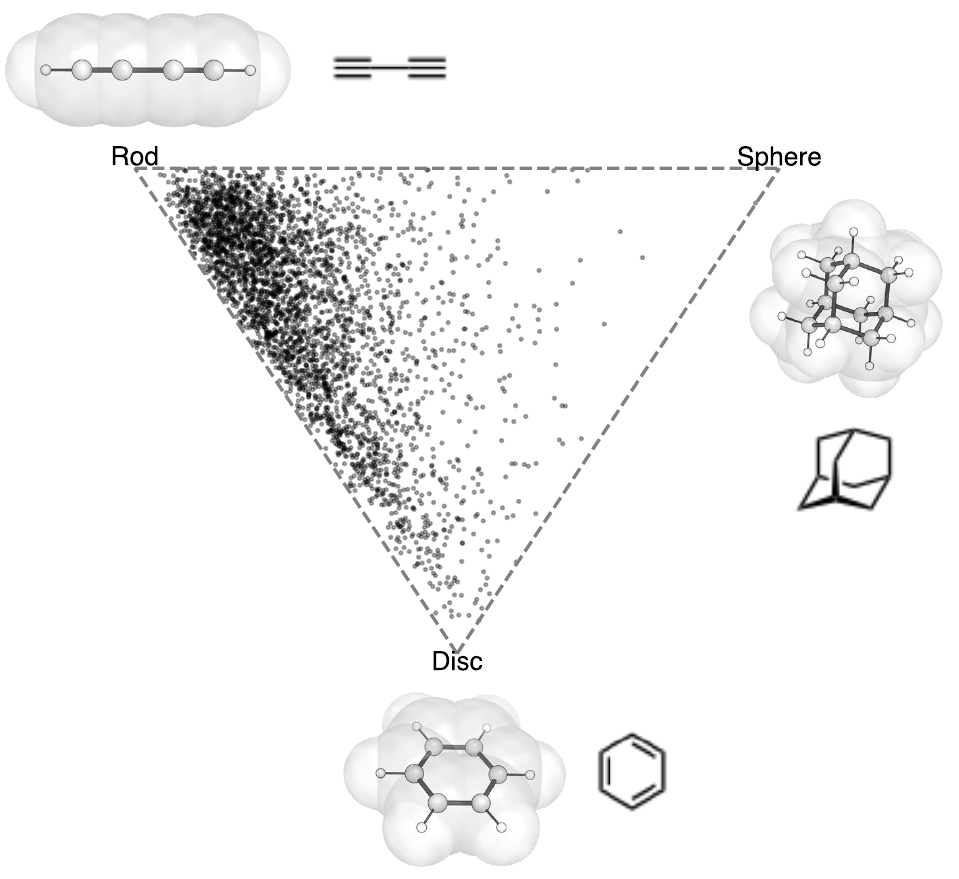
\includegraphics[width=0.72\linewidth]{figures/CH4-pmi.png}
  \caption{
    Schematic molecular shape space based on principal moments of inertia.
    The same idea of molecular distance can be applied to geometrical rather than steric--electronic descriptors.
  }
  \label{fig4-5:pmi-shape-space}
\end{figure}

The Tolman and shape-space examples describe different molecular questions and therefore arrange molecules differently.
This is an important feature rather than a failure of chemical-space analysis: the representation determines which molecular relationships are emphasised.

Two-dimensional maps are easy to inspect because both descriptor axes can be drawn directly.
Modern ligand libraries contain many steric, electronic, geometric, and whole-molecule descriptors, so the corresponding ligand space \keypoint{multidimensional}.
For example, \textit{kraken} combines large numbers of calculated descriptors for organophosphorus ligands rather than relying on one steric and one electronic coordinate.
Every descriptor adds another axis and every ligand remains a point defined by its descriptor values.
The practical problem is that a space containing many descriptor axes can no longer be visualised directly.
This motivates \keypoint{dimensionality reduction}: constructing a lower-dimensional view that retains useful structure from the original descriptor space.

\section{Dimensionality reduction}

Tolman's ligand map can be drawn directly because it contains only two descriptor axes.
Modern descriptor libraries contain many steric, electronic, and geometric, so the corresponding chemical space cannot be inspected directly.
\keypoint{Dimensionality reduction} constructs a lower-dimensional representation that preserves selected structure from the original descriptor space.
The resulting axes need not correspond to individual molecular descriptors, and information is generally lost when a high-dimensional space is projected into only two or three dimensions.

\subsection{Principal component analysis}

\keypoint{Principal component analysis (PCA)} constructs new orthogonal axes, called principal components, from linear combinations of the original descriptors.\mcite{Pearson1901}
The first principal component is chosen to capture the greatest possible variance in the dataset.
The second captures the greatest remaining variance while being orthogonal to the first, and subsequent components follow the same principle.

Each principal component is a weighted combination of the original descriptors,

\begin{equation}
  \mathrm{PC}_k
  =
  w_{k1}x_1
  + w_{k2}x_2
  + \cdots
  + w_{kp}x_p.
\end{equation}

The coefficients $w_{kj}$ describe how strongly descriptor $j$ contributes to principal component $k$.
PCA therefore rotates the original descriptor coordinate system to obtain new axes that summarise the major directions of variation in the dataset.

\solution{8cm}{
% \begin{figure}[htbp]
  \centering
  \resizebox{\linewidth}{!}{%
    \begin{tikzpicture}[
        transform shape,
        axis/.style={draw=darkGrey,line width=1.5pt,->,>=Stealth},
        datum/.style={fill=darkBlue,draw=darkBlue},
        pc/.style={draw=darkRed,line width=2.5pt,->,>=Stealth},
        bad/.style={draw=darkGreen,line width=2.5pt,->,>=Stealth},
        project/.style={draw=darkGrey,dashed,line width=1.0pt},
        spread/.style={draw=darkGrey,line width=1.5pt,<->,>=Stealth},
        label/.style={font=\small\sffamily,text=darkGrey,align=center},
        title/.style={font=\sffamily,text=darkGrey,align=center}
      ]

      \path[use as bounding box] (0,-0.5) rectangle (17.3,6.7);

      % Original 2D descriptor space
      \node[title] at (4.1,6.25) {Original descriptor space};
      \draw[axis] (0.8,0.9) -- (7.8,0.9);
      \draw[axis] (0.8,0.9) -- (0.8,5.7);
      \node[label,anchor=east] at (7.65,0.43) {$x_1$};
      \node[label,rotate=90] at (0.28,4.85) {$x_2$};

      % Elongated correlated cloud
      \foreach \x/\y in {
        1.55/1.50,1.95/1.72,2.35/1.82,2.65/2.13,
        3.05/2.18,3.35/2.47,3.70/2.52,4.05/2.88,
        4.40/2.95,4.75/3.23,5.10/3.38,5.42/3.63,
        5.78/3.78,6.10/4.05,6.48/4.13,6.80/4.48,
        2.55/1.75,3.85/2.95,5.25/3.08,6.15/4.42
      } {
        \fill[datum] (\x,\y) circle (3.3pt);
      }

      % Directions through the cloud
      \draw[pc] (2.0,1.50) -- (6.75,4.70);
      \node[label,text=darkRed,anchor=west] at (6.78,4.72)
        {large variance};

      \draw[bad] (3.00,4.20) -- (5.20,1.25);
      \node[label,text=darkGreen,anchor=west] at (1.28,4.65)
        {small variance};

      % Arrow to one-dimensional projections
      \draw[axis] (8.25,3.25) -- (9.15,3.25);

      % Good projection
      \node[title] at (13.20,6.25) {Projected onto one axis};
      \draw[axis] (9.65,4.55) -- (16.55,4.55);
      \foreach \x in {10.00,10.30,10.68,11.05,11.45,11.85,12.25,12.72,13.15,13.60,14.05,14.48,14.90,15.28,15.70,16.00} {
        \fill[datum] (\x,4.55) circle (3.3pt);
      }
      \draw[spread] (10.00,5.15) -- (16.00,5.15);
      \node[label,text=darkRed] at (13.00,5.55)
        {projection retains broad variation};

      % Poor projection
      \draw[axis] (9.65,1.70) -- (16.55,1.70);
      \foreach \x in {12.10,12.26,12.37,12.49,12.62,12.72,12.84,12.96,13.08,13.20,13.31,13.43,13.54,13.66,13.78,13.91} {
        \fill[datum] (\x,1.70) circle (3.3pt);
      }
      \draw[spread] (12.10,2.30) -- (13.91,2.30);
      \node[label,text=darkGreen] at (13.00,2.70)
        {projection collapses variation};

      \node[label] at (13.00,0.82)
        {PCA selects directions that maximise retained variance};

    \end{tikzpicture}%
  }
%   \caption{
%     Dimensionality reduction depends on the direction of projection.
%     Projecting the same descriptor data along different directions preserves different amounts of variation.
%     Principal component analysis selects orthogonal directions that retain the greatest variance in the dataset.
%   }
%   \label{fig4-6:pca-projection}
% \end{figure}
  \vspace{2em}
  \textbf{original axes}
  $=$
  molecular descriptors

  \textbf{new PCA axes}
  $=$
  orthogonal descriptors explaining most variance

}

After PCA, each molecule has a coordinate along each principal component.
These coordinates are the \keypoint{scores}, and plotting the scores of the first two principal components produces the familiar PCA map.
The descriptor coefficients used to construct each principal component are the \keypoint{loadings}.
Loadings allow the new axes to be interpreted in terms of the original molecular descriptors and are therefore essential when a chemical interpretation of a PCA map is required.

\begin{figure}[htbp]
  \centering

  \resizebox{\linewidth}{!}{%
    \begin{tikzpicture}[
        transform shape,
        axis/.style={draw=darkGrey,line width=1.5pt,->,>=Stealth},
        datum/.style={fill=darkBlue,draw=darkBlue},
        loading/.style={draw=darkRed,line width=2.3pt,->,>=Stealth},
        loadingtwo/.style={draw=darkGreen,line width=2.3pt,->,>=Stealth},
        guide/.style={draw=darkGrey,dashed,line width=1.0pt},
        label/.style={font=\small\sffamily,text=darkGrey,align=center},
        title/.style={font=\sffamily,text=darkGrey,align=center}
      ]

      \path[use as bounding box] (0,-0.5) rectangle (17.3,6.8);

      % Scores plot
      \node[title] at (4.15,6.30) {Scores: where are the molecules?};
      \draw[axis] (0.8,3.20) -- (7.75,3.20);
      \draw[axis] (4.15,0.75) -- (4.15,5.90);
      \node[label,anchor=east] at (7.60,2.73) {PC1};
      \node[label,rotate=90] at (3.58,5.10) {PC2};

      \foreach \x/\y in {
        1.55/2.10,2.05/2.55,2.45/1.72,2.82/2.88,
        3.35/3.52,3.65/4.15,4.05/3.82,
        4.60/3.42,5.05/4.20,5.35/3.72,
        5.92/2.55,6.35/2.02,6.78/2.82
      } {
        \fill[datum] (\x,\y) circle (3.6pt);
      }

      \node[label,anchor=west] at (2.15,0)
        {each point = one molecule};

      % Divider arrow
      \draw[axis] (8.20,3.20) -- (9.05,3.20);

      % Loading plot
      \node[title] at (13.05,6.30) {Loadings: what defines the axes?};
      \draw[axis] (9.65,3.20) -- (16.55,3.20);
      \draw[axis] (13.05,0.75) -- (13.05,5.90);
      \node[label,anchor=east] at (16.40,2.73) {PC1};
      \node[label,rotate=90] at (12.48,5.10) {PC2};

      % Descriptor loading vectors
      \draw[loading] (13.05,3.20) -- (15.72,4.72);
      \node[label,text=darkRed,anchor=west] at (15.80,4.76)
        {$x_1$: steric};

      \draw[loading] (13.05,3.20) -- (15.45,2.02);
      \node[label,text=darkRed,anchor=west] at (15.52,1.98)
        {$x_2$: size};

      \draw[loadingtwo] (13.05,3.20) -- (11.15,5.00);
      \node[label,text=darkGreen,anchor=east] at (11.05,5.05)
        {$x_3$: electronic};

      \draw[loadingtwo] (13.05,3.20) -- (10.60,2.15);
      \node[label,text=darkGreen,anchor=east] at (10.50,2.10)
        {$x_4$: polarity};

      \node[label] at (13.05,0)
        {arrows describe descriptor contributions};

    \end{tikzpicture}%
  }

  \caption{
    Relationship between PCA scores and loadings.
    Scores describe the positions of molecules in principal-component space.
    Loadings describe how the original descriptors contribute to each principal component and  provide a route to chemical interpretation of the new axes.
  }
  \label{fig4:pca-scores-loadings}
\end{figure}

\solution{3cm}{%
  \centering

  \textbf{scores}
  $\longrightarrow$
  where are the molecules?

  \vspace{0.8em}

  \textbf{loadings}
  $\longrightarrow$
  which descriptors define those directions?
}

\subsection{Explained variance}

Reducing dimensionality necessarily discards some information.
The \keypoint{explained variance} of a principal component reports how much of the total variation in the original dataset is represented along that component.
The cumulative explained variance of the retained components therefore provides one measure of how much information is preserved in a lower-dimensional map.

A two-dimensional PCA plot may be visually convenient while representing only part of the variation in the original descriptor space.
The percentage of variance explained by the displayed components should therefore be reported and considered when interpreting apparent distances, groups, or gaps.

\begin{conceptbox}
  \keypoint{A PCA map is a projection, not the chemical space itself.}
  Apparent molecular relationships in a two-dimensional scores plot are useful only to the extent that the retained components capture the variation relevant to the chemical question.
  Loadings and explained variance are therefore part of the interpretation, not optional statistical details.
\end{conceptbox}

\subsection{Nonlinear maps}

Other dimensionality-reduction methods, including t-SNE and UMAP, can produce useful low-dimensional maps when relationships in the original descriptor space are not well represented by linear projections.
These methods are particularly useful for visualising local neighbourhoods and complex high-dimensional structure, but their map axes do not have the direct descriptor-based interpretation of PCA loadings.
The geometry of a nonlinear map can also depend strongly on the method and its settings.
Distances and cluster separation in a two-dimensional visualisation should not automatically be interpreted as distances in the original descriptor space.

\section{Mapping chemical spaces}

\subsection{Ligand Knowledge Bases (LKB)}

Tolman's map shows how two chemically meaningful parameters can organise ligands into a useful property space.
Modern ligand datasets extend the same idea by combining many calculated steric, electronic, and geometric descriptors.
Dimensionality reduction then provides a way to visualise the dominant patterns within this higher-dimensional space.

\begin{figure}[htbp]
  \centering
  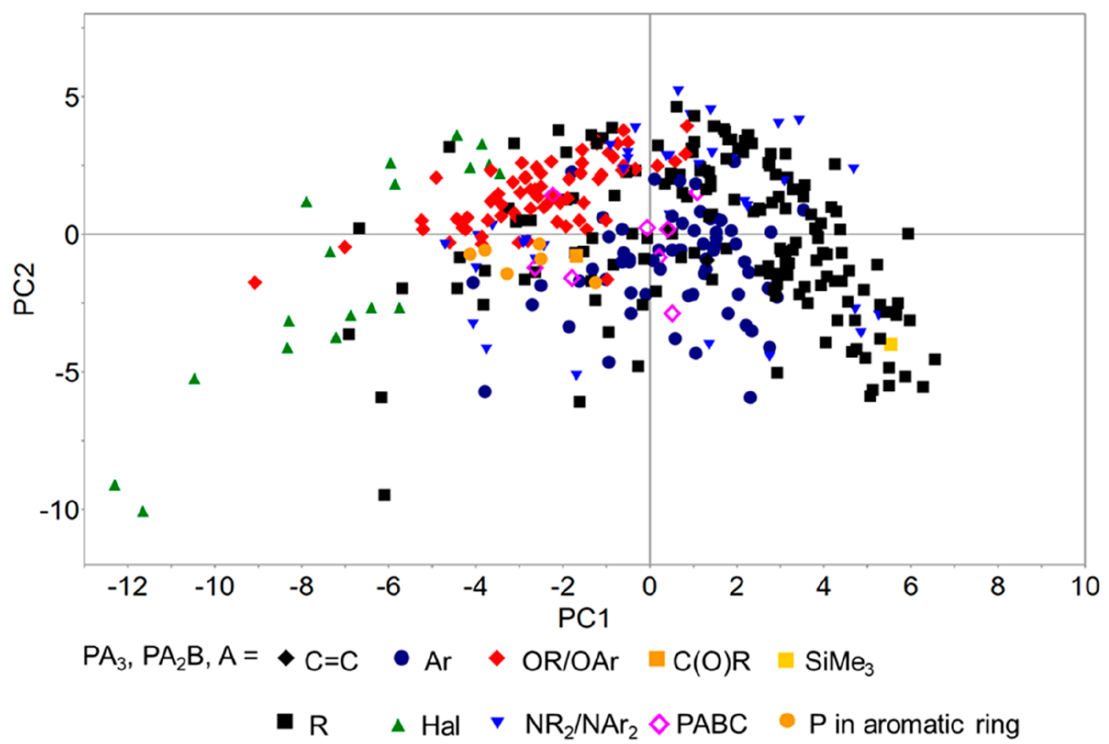
\includegraphics[width=0.88\linewidth]{figures/CH4-LKB-P.png}
  \caption{
    PCA map of phosphine ligand knowledge map. There are 28 descriptors calculated for 366 ligands; \textit{ca.} 62\% of variance is captured. 
  }
  \label{fig4-6:fey-lkb-p}
\end{figure}

Work by Fey and co-workers provides a useful modern continuation of the Tolman approach.\mcite{Durand2021}
Ligand knowledge bases collect steric and electronic descriptors for large sets of ligands and use principal component analysis to obtain lower-dimensional maps of ligand property space (Fig.~\ref{fig4-6:fey-lkb-p}).
A useful feature of this representation is that molecular structure is not used as the sole definition of similarity.
Ligands with different structural motifs may occupy similar regions when their calculated properties are similar, while apparently related ligands can separate when they differ strongly in the descriptors that define the map.
A diverse selection of ligands can be designed to span different regions of property space rather than simply collecting ligands with visibly different structures.

\begin{conceptbox}
If two candidate ligands occupy almost the same region of a chosen property space, testing both may provide  little additional coverage of that representation.
Selecting ligands from distinct regions can provide a broader survey of steric and electronic effects using a smaller experimental set.
\end{conceptbox}

\subsection{Exploring solvent space}

Solvents provide another intuitive example because solvent choice depends on several physical and chemical properties simultaneously.
A solvent can also be represented as a point in a multidimensional property space.

\solution{4cm}{%

Properties relevant to solvent comparison may include:
\begin{itemize}
  \item polarity
  \item boiling point
  \item environmental safety
  \item $\cdots$
\end{itemize}
}


The \keypoint{ACS Green Chemistry Institute Pharmaceutical Roundtable} is an interactive solvent tool based on principal component analysis of 70 solvent properties.\mcite{Alder2016}
The tool uses a PCA map to organise solvents according to their physical and chemical similarity and supplements this map with information including functional groups, physical properties, and environmental data.
The map provides a practical way to search for alternatives to a familiar solvent (Fig.~\ref{fig4-7:acs-solvent-replacement}).

\begin{figure}[htbp]
  \centering
  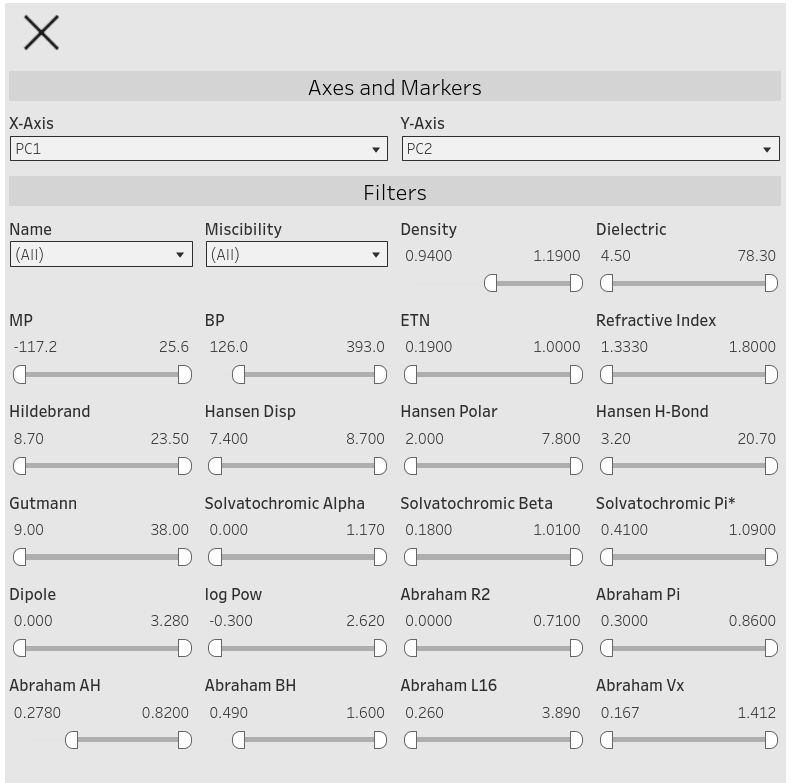
\includegraphics[width=0.45\linewidth]{figures/CH4-ACS-settings.png}
  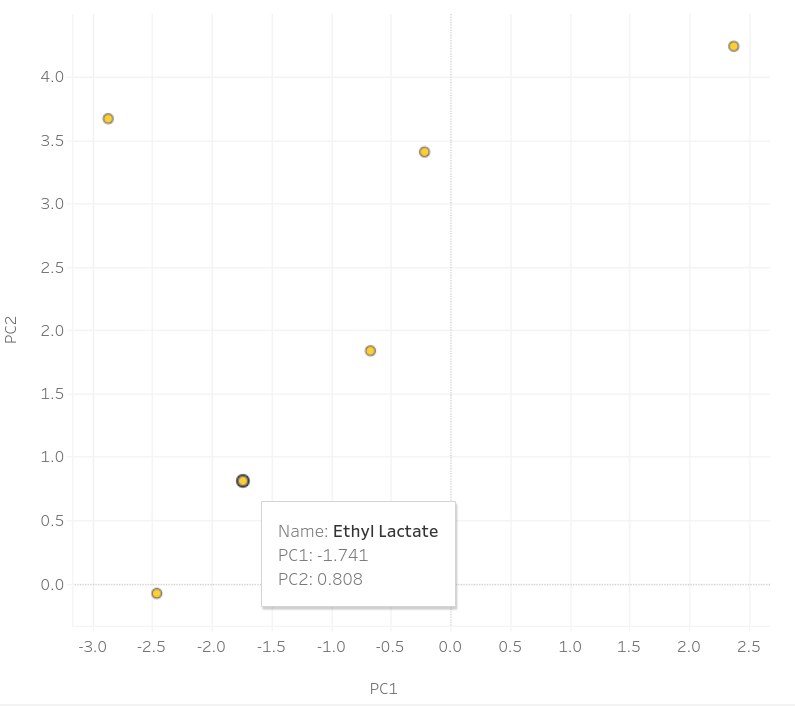
\includegraphics[width=0.45\linewidth]{figures/CH4-ACS-results.png}
  \caption{
    Example use of the ACS Solvent Tool to identify candidate replacements for a solvent.
  }
  \label{fig4-7:acs-solvent-replacement}
\end{figure}

\section{Clustering and representative selection}

Chemical-space maps can reveal densely populated regions, isolated molecules, and gaps in the sampled space.
When the number of possible molecules is much larger than the number of experiments that can be performed, these patterns can be used to select a smaller and more informative subset.
\keypoint{Clustering} groups molecules according to their proximity in a chosen representation.
Unlike the regression and classification problems introduced earlier, clustering does not require a target property: the groups are identified from the molecular representation itself.

\begin{conceptbox}
  \keypoint{Clusters are properties of a representation, not intrinsic labels carried by molecules.}
  Changing the descriptors or the way distances are calculated can change which molecules are grouped together.
\end{conceptbox}

\solution{8.0cm}{%
  \centering

  \resizebox{\linewidth}{!}{%
    \begin{tikzpicture}[
        transform shape,
        axis/.style={draw=darkGrey,line width=1.4pt,->,>=Stealth},
        arrow/.style={draw=darkGrey,line width=2.0pt,->,>=Stealth},
        bluepoint/.style={fill=darkBlue,draw=darkBlue},
        redpoint/.style={fill=darkRed,draw=darkRed},
        greenpoint/.style={fill=darkGreen,draw=darkGreen},
        greyPoint/.style={fill=darkGrey,draw=darkGrey},
        centroid/.style={fill=white,draw=darkGrey,line width=1.6pt},
        representative/.style={fill=darkYellow,draw=darkGrey,line width=1.1pt},
        clusterblue/.style={fill=paleBlue,draw=darkBlue,line width=1.5pt,opacity=0.55},
        clusterred/.style={fill=paleRed,draw=darkRed,line width=1.5pt,opacity=0.55},
        clustergreen/.style={fill=paleGreen,draw=darkGreen,line width=1.5pt,opacity=0.55},
        label/.style={font=\small\sffamily,text=darkGrey,align=center},
        title/.style={font=\sffamily,text=darkGrey,align=center}
      ]

      \path[use as bounding box] (0,-0.55) rectangle (17.3,7.3);

      % ---------------------------------------------------------------------
      % Panel 1: chemical space
      % ---------------------------------------------------------------------
      \node[title] at (2.6,6.80) {Chemical space};
      \draw[axis] (0.55,1.15) -- (4.65,1.15);
      \draw[axis] (0.55,1.15) -- (0.55,6.15);
      \node[label,anchor=east] at (4.55,0.72) {PC1};
      \node[label,rotate=90] at (0.12,5.40) {PC2};

      % Three latent groups, initially all shown identically.
      \foreach \x/\y in {
        1.00/2.10,1.28/2.36,1.55/2.02,1.72/2.55,1.95/2.28,
        2.52/4.55,2.78/4.85,3.02/4.48,3.18/5.10,3.42/4.72,
        3.02/2.25,3.30/2.45,3.56/2.13,3.78/2.67,4.05/2.37
      } {
        \fill[greyPoint] (\x,\y) circle (3.0pt);
      }

      % Arrow
      \draw[arrow] (4.95,3.65) -- (6.00,3.65);
      \node[label] at (5.47,4.10) {cluster};

      % ---------------------------------------------------------------------
      % Panel 2: clustered space
      % ---------------------------------------------------------------------
      \node[title] at (8.55,6.80) {Clusters};
      \draw[axis] (6.35,1.15) -- (10.75,1.15);
      \draw[axis] (6.35,1.15) -- (6.35,6.15);
      \node[label,anchor=east] at (10.65,0.72) {PC1};
      \node[label,rotate=90] at (5.92,5.40) {PC2};

      % Pale cluster regions first.
      \fill[clusterblue]
        plot[smooth cycle,tension=0.8] coordinates {
          (6.72,1.72) (7.45,1.62) (8.02,2.05) (7.88,2.87) (7.05,3.05) (6.62,2.48)
        };
      \fill[clusterred]
        plot[smooth cycle,tension=0.8] coordinates {
          (7.86,4.05) (8.35,3.86) (9.10,4.05) (9.46,4.90) (8.92,5.55) (8.08,5.40)
        };
      \fill[clustergreen]
        plot[smooth cycle,tension=0.8] coordinates {
          (8.68,1.72) (9.32,1.58) (10.20,1.95) (10.42,2.74) (9.78,3.18) (8.92,2.94)
        };

      \foreach \x/\y in {6.80/2.10,7.08/2.36,7.35/2.02,7.52/2.55,7.75/2.28}
        {\fill[bluepoint] (\x,\y) circle (3.0pt);}
      \foreach \x/\y in {8.02/4.55,8.28/4.85,8.52/4.48,8.68/5.10,8.92/4.72}
        {\fill[redpoint] (\x,\y) circle (3.0pt);}
      \foreach \x/\y in {9.02/2.25,9.30/2.45,9.56/2.13,9.78/2.67,10.05/2.37}
        {\fill[greenpoint] (\x,\y) circle (3.0pt);}

      % Centroids as open circles.
      \draw[centroid] (7.30,2.28) circle (6.0pt);
      \draw[centroid] (8.50,4.74) circle (6.0pt);
      \draw[centroid] (9.54,2.37) circle (6.0pt);

      % Arrow
      \draw[arrow] (11.05,3.65) -- (12.10,3.65);
      \node[label] at (11.58,4.10) {select};

      % ---------------------------------------------------------------------
      % Panel 3: representative molecules
      % ---------------------------------------------------------------------
      \node[title] at (14.75,6.80) {Representative molecules};
      \draw[axis] (12.45,1.15) -- (16.90,1.15);
      \draw[axis] (12.45,1.15) -- (12.45,6.15);
      \node[label,anchor=east] at (16.80,0.72) {PC1};
      \node[label,rotate=90] at (12.02,5.40) {PC2};

      % Original space faded into context.
      \foreach \x/\y in {
        12.90/2.10,13.18/2.36,13.45/2.02,13.62/2.55,13.85/2.28,
        14.12/4.55,14.38/4.85,14.62/4.48,14.78/5.10,15.02/4.72,
        15.12/2.25,15.40/2.45,15.66/2.13,15.88/2.67,16.15/2.37
      } {
        \fill[paleGrey] (\x,\y) circle (2.6pt);
      }

      % Selected nearest-to-centroid representatives.
      \fill[representative] (13.45,2.02) circle (5.2pt);
      \fill[representative] (14.62,4.48) circle (5.2pt);
      \fill[representative] (15.40,2.45) circle (5.2pt);

      \node[label,anchor=west] at (13.75,3.45)
        {one molecule selected\\from each region};

    \end{tikzpicture}%
  }
}

\subsection{Reaction scope as a selection problem}

Representative selection is also relevant when demonstrating the scope of a new synthetic method.
Substrate scopes are rarely unbiased samples of chemical space. 
A conventional substrate scope can be influenced by availability, familiarity, or the expectation that particular substrates will succeed.
\keypoint{Selection bias} arises because substrates are typically chosen based on availability, precedent, expected reactivity, or to demonstrate particular functional-group tolerance, while \keypoint{reporting bias} can arise when successful or informative reactions are preferentially reported over unsuccessful examples.
Systematic data-driven selection of diverse substrates provides one route towards constructing more representative tests of reaction generality.
Rana and co-workers developed a standardised substrate-selection strategy in which unsupervised learning is used to identify an unbiased substrate scope (Fig.~\ref{fig4:glorius-scope-1} and Fig.~\ref{fig4:glorius-scope-2}).\mcite{Rana2024}

\begin{figure}[htbp]
  \centering
  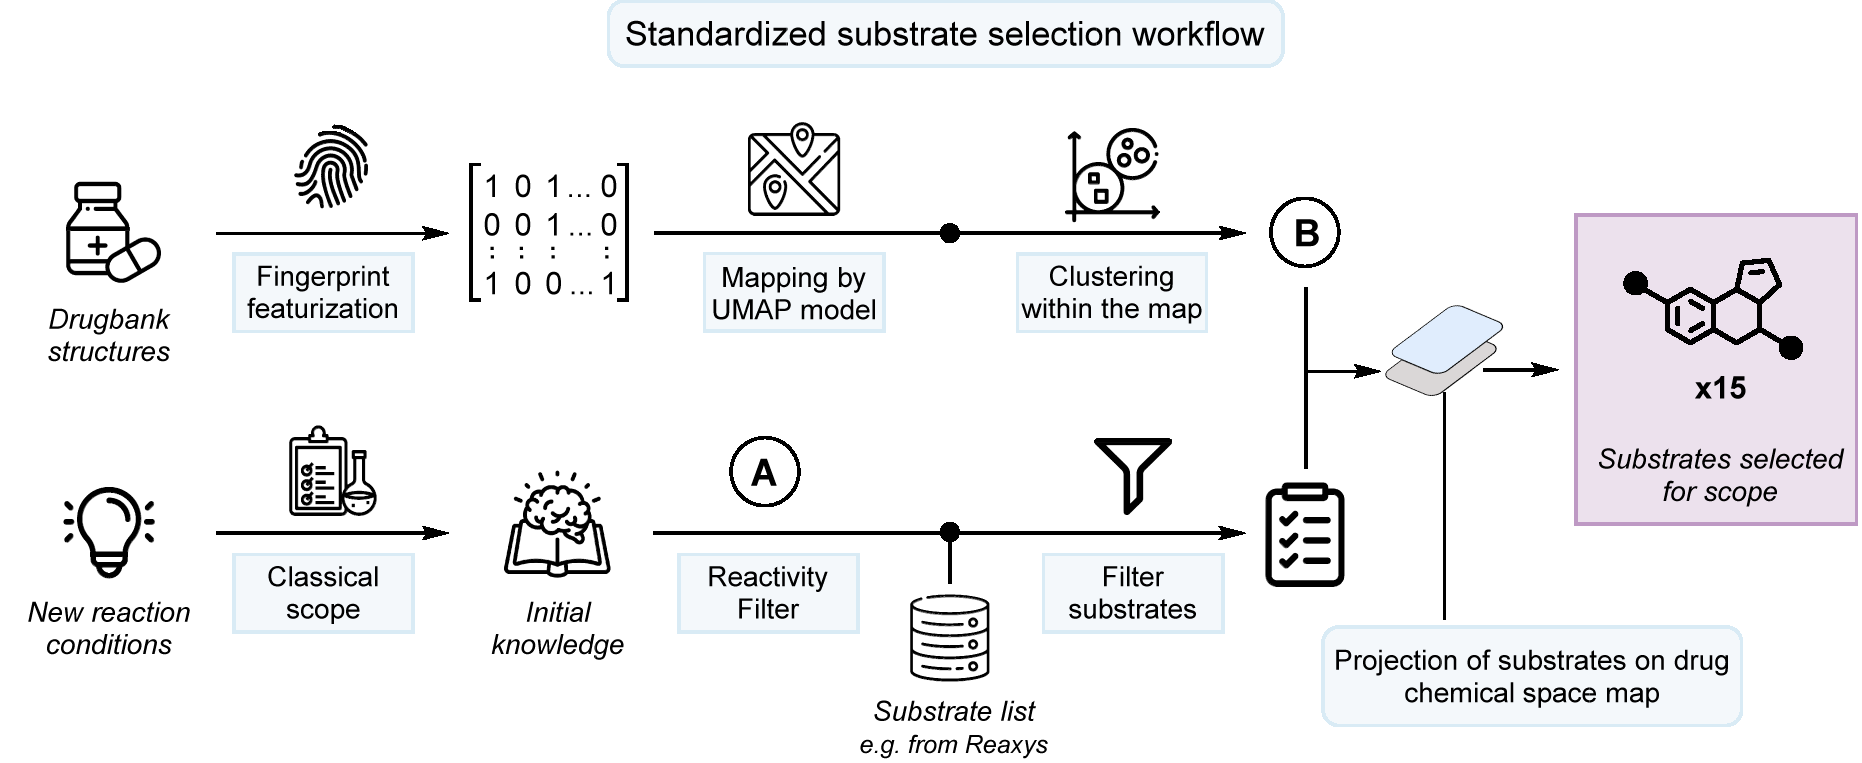
\includegraphics[width=\linewidth]{figures/CH4-glorius-1.png}
  \caption{
   Unbiased substrate scope selection strategy for evaluating reaction generality.
  }
  \label{fig4:glorius-scope-1}
\end{figure}

\begin{figure}[htbp]
  \centering
  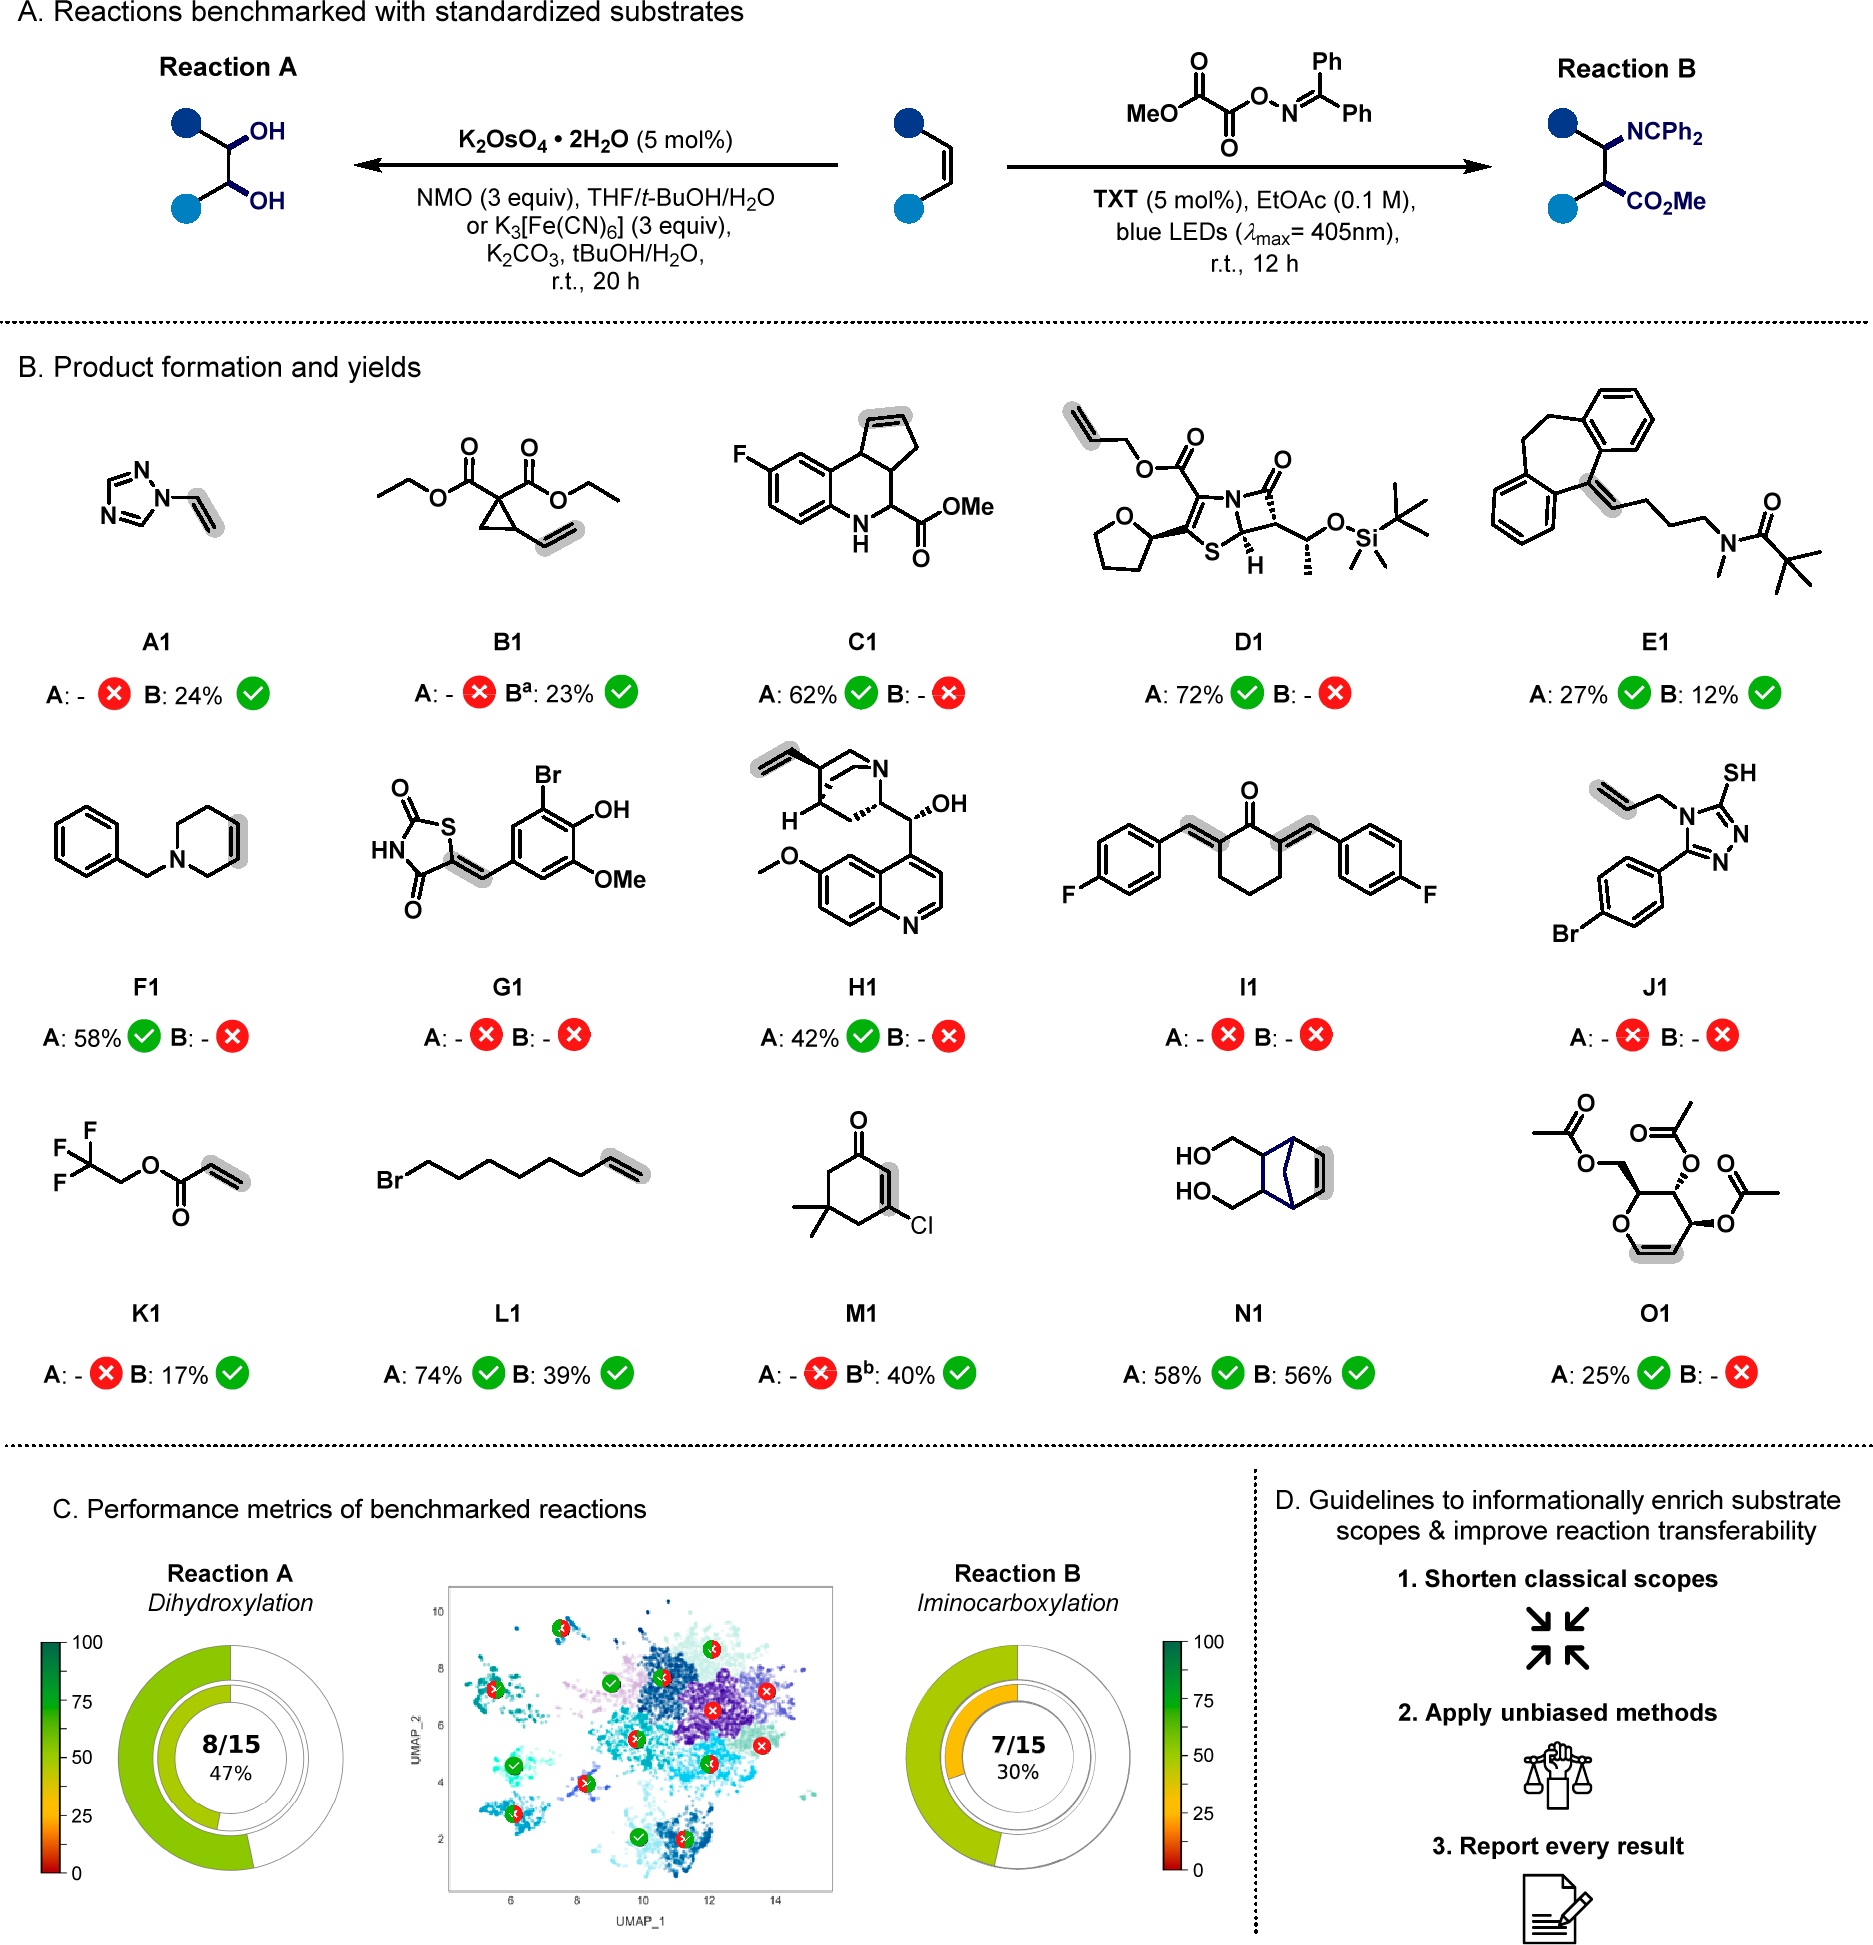
\includegraphics[width=\linewidth]{figures/CH4-glorius-2.png}
  \caption{
    Resulting generality assessment of two olefin functionalisation reactions.
  }
  \label{fig4:glorius-scope-2}
\end{figure}


\section{Summary}

Molecular descriptors convert selected aspects of chemical structure and properties into numerical representations.
Classical physical-organic parameters such as Hammett, Taft, and Tolman descriptors provide early examples of this idea, while modern descriptor libraries extend it to large collections of steric, electronic, geometric, and physicochemical properties.
Distances and similarities between these representations provide a quantitative definition of molecular neighbourhoods.
Dimensionality reduction allows high-dimensional molecular spaces to be visualised, while scores, loadings, and explained variance are required to interpret those projections critically.
Real ligand and solvent maps show how these methods can support chemical comparison and candidate selection.
Clustering and representative selection then turn a chemical-space map into an experimental-design tool.
The next chapter considers how descriptor-rich datasets can be converted into quantitative models of chemical reactivity and selectivity, and asks when such models provide chemical understanding rather than prediction alone.

% % !TeX root = ../notes.tex

\chapter{Modern molecular descriptors}

\section{Introduction}

This chapter develops the role of modern molecular descriptors within the course narrative.

\begin{insightbox}
\textbf{Chapter thread:} motivation; method; chemical application; limitations; connection.
\end{insightbox}

\section{From representation to descriptor}

\begin{conceptbox}
\textbf{Keywords:} descriptor; feature; information.
\end{conceptbox}

\subsection{Representation, descriptor and feature}

% Add explanatory text, figure, worked example or fill-in gap here.

\subsection{What should the model know?}

% Add explanatory text, figure, worked example or fill-in gap here.

\section{Classical physical-organic descriptors}

\begin{conceptbox}
\textbf{Keywords:} electronic effects; steric effects; LFER.
\end{conceptbox}

\subsection{Hammett substituent constants}

% Add explanatory text, figure, worked example or fill-in gap here.

\subsection{Taft parameters}

% Add explanatory text, figure, worked example or fill-in gap here.

\subsection{Scope and transferability}

% Add explanatory text, figure, worked example or fill-in gap here.

\section{Steric descriptors}

\begin{methodbox}
\textbf{Keywords:} Sterimol; buried volume; shape.
\end{methodbox}

\subsection{Cone angle and A-values}

% Add explanatory text, figure, worked example or fill-in gap here.

\subsection{Sterimol parameters}

% Add explanatory text, figure, worked example or fill-in gap here.

\subsection{Buried volume}

% Add explanatory text, figure, worked example or fill-in gap here.

\subsection{Solvent-accessible surface area}

% Add explanatory text, figure, worked example or fill-in gap here.

\section{Conformational dependence}

\begin{warningbox}
\textbf{Keywords:} conformers; weighting; flexibility.
\end{warningbox}

\subsection{Single structures and ensembles}

% Add explanatory text, figure, worked example or fill-in gap here.

\subsection{Minimum, maximum and Boltzmann-weighted values}

% Add explanatory text, figure, worked example or fill-in gap here.

\subsection{Flexibility as information}

% Add explanatory text, figure, worked example or fill-in gap here.

\section{Electronic descriptors}

\begin{methodbox}
\textbf{Keywords:} HOMO; charges; polarity.
\end{methodbox}

\subsection{Frontier-orbital energies}

% Add explanatory text, figure, worked example or fill-in gap here.

\subsection{Charges and electrostatic potentials}

% Add explanatory text, figure, worked example or fill-in gap here.

\subsection{Dipole and polarisability}

% Add explanatory text, figure, worked example or fill-in gap here.

\subsection{Vibrational and spectroscopic quantities}

% Add explanatory text, figure, worked example or fill-in gap here.

\section{Descriptor generation at scale}

\begin{warningbox}
\textbf{Keywords:} cost; level of theory; standardisation.
\end{warningbox}

\subsection{Experimental, DFT and semi-empirical routes}

% Add explanatory text, figure, worked example or fill-in gap here.

\subsection{Computational cost and reproducibility}

% Add explanatory text, figure, worked example or fill-in gap here.

\subsection{Descriptor libraries and Kraken-type spaces}

% Add explanatory text, figure, worked example or fill-in gap here.

\section{Fingerprints versus physicochemical descriptors}

\begin{insightbox}
\textbf{Keywords:} fingerprints; interpretability; sparsity.
\end{insightbox}

\subsection{Interpretability}

% Add explanatory text, figure, worked example or fill-in gap here.

\subsection{Dimensionality and sparsity}

% Add explanatory text, figure, worked example or fill-in gap here.

\subsection{2D and 3D information}

% Add explanatory text, figure, worked example or fill-in gap here.

\section{Learned representations}

\begin{conceptbox}
\textbf{Keywords:} GNN; message passing; representation learning.
\end{conceptbox}

\subsection{Attributed molecular graphs}

% Add explanatory text, figure, worked example or fill-in gap here.

\subsection{Message passing}

% Add explanatory text, figure, worked example or fill-in gap here.

\subsection{Hand-crafted versus learned features}

% Add explanatory text, figure, worked example or fill-in gap here.

\section{Choosing descriptors for a task}

\begin{methodbox}
\textbf{Keywords:} task fit; selection; leakage.
\end{methodbox}

\subsection{Similarity search}

% Add explanatory text, figure, worked example or fill-in gap here.

\subsection{Mechanistic modelling}

% Add explanatory text, figure, worked example or fill-in gap here.

\subsection{Large-data prediction}

% Add explanatory text, figure, worked example or fill-in gap here.

\subsection{Avoiding redundant and leaked features}

% Add explanatory text, figure, worked example or fill-in gap here.

\section{Chapter summary and practice}

\begin{notebox}
\textbf{Keywords:} compare; select; justify.
\end{notebox}

\subsection{Compare descriptor families}

% Add explanatory text, figure, worked example or fill-in gap here.

\subsection{Design a feature set}

% Add explanatory text, figure, worked example or fill-in gap here.

\section{Summary}

\begin{notebox}
\textbf{Key take-away:} complete after drafting the chapter.
\end{notebox}

\section{Questions for review}

\solution{4cm}{% Add lecturer solution here.
}

% % !TeX root = ../notes.tex

\chapter{Reaction optimisation: OVAT, DoE and Bayesian optimisation}

\section{Introduction}

This chapter develops the role of reaction optimisation: ovat, doe and bayesian optimisation within the course narrative.

\begin{insightbox}
\textbf{Chapter thread:} motivation; method; chemical application; limitations; connection.
\end{insightbox}

\section{Defining an optimisation problem}

\begin{conceptbox}
\textbf{Keywords:} factors; constraints; objective.
\end{conceptbox}

\subsection{Variables, constraints and objectives}

% Add explanatory text, figure, worked example or fill-in gap here.

\subsection{Continuous and categorical factors}

% Add explanatory text, figure, worked example or fill-in gap here.

\subsection{What counts as an optimum?}

% Add explanatory text, figure, worked example or fill-in gap here.

\section{One variable at a time}

\begin{warningbox}
\textbf{Keywords:} OVAT; interactions; local optimum.
\end{warningbox}

\subsection{The OVAT workflow}

% Add explanatory text, figure, worked example or fill-in gap here.

\subsection{Strengths and limitations}

% Add explanatory text, figure, worked example or fill-in gap here.

\subsection{Hidden interactions}

% Add explanatory text, figure, worked example or fill-in gap here.

\section{Factorial experiments}

\begin{methodbox}
\textbf{Keywords:} factorial; effects; interactions.
\end{methodbox}

\subsection{Factors and levels}

% Add explanatory text, figure, worked example or fill-in gap here.

\subsection{Main effects and interactions}

% Add explanatory text, figure, worked example or fill-in gap here.

\subsection{Full and fractional factorial designs}

% Add explanatory text, figure, worked example or fill-in gap here.

\section{Response surfaces and design of experiments}

\begin{methodbox}
\textbf{Keywords:} DoE; response surface; curvature.
\end{methodbox}

\subsection{Empirical response surfaces}

% Add explanatory text, figure, worked example or fill-in gap here.

\subsection{Curvature and non-linear response}

% Add explanatory text, figure, worked example or fill-in gap here.

\subsection{Efficient information gathering}

% Add explanatory text, figure, worked example or fill-in gap here.

\section{Sequential experimentation}

\begin{insightbox}
\textbf{Keywords:} adaptive design; iteration; information.
\end{insightbox}

\subsection{Learning from each round}

% Add explanatory text, figure, worked example or fill-in gap here.

\subsection{Batch and sequential choices}

% Add explanatory text, figure, worked example or fill-in gap here.

\section{Bayesian optimisation}

\begin{methodbox}
\textbf{Keywords:} surrogate; acquisition; uncertainty.
\end{methodbox}

\subsection{Surrogate models}

% Add explanatory text, figure, worked example or fill-in gap here.

\subsection{Prediction and uncertainty}

% Add explanatory text, figure, worked example or fill-in gap here.

\subsection{Acquisition functions}

% Add explanatory text, figure, worked example or fill-in gap here.

\subsection{Exploration and exploitation}

% Add explanatory text, figure, worked example or fill-in gap here.

\section{Green multi-objective optimisation}

\begin{insightbox}
\textbf{Keywords:} PMI; sustainability; Pareto front.
\end{insightbox}

\subsection{Yield, selectivity and productivity}

% Add explanatory text, figure, worked example or fill-in gap here.

\subsection{PMI, waste, energy, hazard and cost}

% Add explanatory text, figure, worked example or fill-in gap here.

\subsection{Pareto trade-offs}

% Add explanatory text, figure, worked example or fill-in gap here.

\section{Failed and infeasible experiments}

\begin{warningbox}
\textbf{Keywords:} failure; feasibility; constraints.
\end{warningbox}

\subsection{Failures as data}

% Add explanatory text, figure, worked example or fill-in gap here.

\subsection{Constraints and safe operating regions}

% Add explanatory text, figure, worked example or fill-in gap here.

\section{Worked reaction-optimisation case study}

\begin{resultbox}
\textbf{Keywords:} conditions; evidence; next experiment.
\end{resultbox}

\subsection{Define the search space}

% Add explanatory text, figure, worked example or fill-in gap here.

\subsection{Compare OVAT, DoE and BO recommendations}

% Add explanatory text, figure, worked example or fill-in gap here.

\subsection{Select the next experiment}

% Add explanatory text, figure, worked example or fill-in gap here.

\section{Chapter summary and practice}

\begin{notebox}
\textbf{Keywords:} choose; trade off; justify.
\end{notebox}

\subsection{Choose an optimisation strategy}

% Add explanatory text, figure, worked example or fill-in gap here.

\subsection{Interpret interactions}

% Add explanatory text, figure, worked example or fill-in gap here.

\subsection{Balance competing objectives}

% Add explanatory text, figure, worked example or fill-in gap here.

\section{Summary}

\begin{notebox}
\textbf{Key take-away:} complete after drafting the chapter.
\end{notebox}

\section{Questions for review}

\solution{4cm}{% Add lecturer solution here.
}

% % !TeX root = ../notes.tex

\chapter{Generating chemical data: high-throughput and flow chemistry}

\section{Introduction}

This chapter develops the role of generating chemical data: high-throughput and flow chemistry within the course narrative.

\begin{insightbox}
\textbf{Chapter thread:} motivation; method; chemical application; limitations; connection.
\end{insightbox}

\section{Why generate data at scale?}

\begin{conceptbox}
\textbf{Keywords:} throughput; information; purpose.
\end{conceptbox}

\subsection{Screening, understanding and optimisation}

% Add explanatory text, figure, worked example or fill-in gap here.

\subsection{Throughput versus information}

% Add explanatory text, figure, worked example or fill-in gap here.

\section{Parallel experimentation}

\begin{methodbox}
\textbf{Keywords:} parallel; liquid handling; scale.
\end{methodbox}

\subsection{Reaction arrays and plates}

% Add explanatory text, figure, worked example or fill-in gap here.

\subsection{Liquid handling and dosing}

% Add explanatory text, figure, worked example or fill-in gap here.

\subsection{Miniaturisation}

% Add explanatory text, figure, worked example or fill-in gap here.

\section{High-throughput reaction screening}

\begin{methodbox}
\textbf{Keywords:} screen; library; coverage.
\end{methodbox}

\subsection{Substrates, ligands, catalysts and conditions}

% Add explanatory text, figure, worked example or fill-in gap here.

\subsection{Experimental design for screening}

% Add explanatory text, figure, worked example or fill-in gap here.

\section{The analytical bottleneck}

\begin{warningbox}
\textbf{Keywords:} analysis; calibration; bottleneck.
\end{warningbox}

\subsection{Sampling strategies}

% Add explanatory text, figure, worked example or fill-in gap here.

\subsection{LC, GC, MS and spectroscopy}

% Add explanatory text, figure, worked example or fill-in gap here.

\subsection{Calibration and automated data processing}

% Add explanatory text, figure, worked example or fill-in gap here.

\section{Flow chemistry fundamentals}

\begin{conceptbox}
\textbf{Keywords:} flow; residence time; steady state.
\end{conceptbox}

\subsection{Reactor architecture}

% Add explanatory text, figure, worked example or fill-in gap here.

\subsection{Residence time}

% Add explanatory text, figure, worked example or fill-in gap here.

\subsection{Mixing and heat transfer}

% Add explanatory text, figure, worked example or fill-in gap here.

\subsection{Steady state}

% Add explanatory text, figure, worked example or fill-in gap here.

\section{Serial experimentation in flow}

\begin{methodbox}
\textbf{Keywords:} serial; lag; inline analysis.
\end{methodbox}

\subsection{Changing conditions}

% Add explanatory text, figure, worked example or fill-in gap here.

\subsection{Accounting for system lag and dispersion}

% Add explanatory text, figure, worked example or fill-in gap here.

\subsection{Integrated analysis}

% Add explanatory text, figure, worked example or fill-in gap here.

\section{Batch versus flow automation}

\begin{insightbox}
\textbf{Keywords:} batch; flow; task fit.
\end{insightbox}

\subsection{Matching architecture to the chemical problem}

% Add explanatory text, figure, worked example or fill-in gap here.

\subsection{Advantages, limitations and hybrid systems}

% Add explanatory text, figure, worked example or fill-in gap here.

\section{Data infrastructure}

\begin{warningbox}
\textbf{Keywords:} provenance; standards; QC.
\end{warningbox}

\subsection{Metadata and provenance}

% Add explanatory text, figure, worked example or fill-in gap here.

\subsection{Machine-readable experimental records}

% Add explanatory text, figure, worked example or fill-in gap here.

\subsection{Failed experiments and quality control}

% Add explanatory text, figure, worked example or fill-in gap here.

\section{Does automation make chemistry greener?}

\begin{insightbox}
\textbf{Keywords:} resource use; waste; evidence.
\end{insightbox}

\subsection{Miniaturisation and process intensification}

% Add explanatory text, figure, worked example or fill-in gap here.

\subsection{Solvent, analytical and consumables burdens}

% Add explanatory text, figure, worked example or fill-in gap here.

\subsection{Measuring rather than assuming greenness}

% Add explanatory text, figure, worked example or fill-in gap here.

\section{Chapter summary and practice}

\begin{notebox}
\textbf{Keywords:} generate; measure; record.
\end{notebox}

\subsection{Design a data-generation workflow}

% Add explanatory text, figure, worked example or fill-in gap here.

\subsection{Identify the bottleneck}

% Add explanatory text, figure, worked example or fill-in gap here.

\subsection{Compare batch and flow}

% Add explanatory text, figure, worked example or fill-in gap here.

\section{Summary}

\begin{notebox}
\textbf{Key take-away:} complete after drafting the chapter.
\end{notebox}

\section{Questions for review}

\solution{4cm}{% Add lecturer solution here.
}

% % !TeX root = ../notes.tex

\chapter{Autonomous and self-driving laboratories}

\section{Introduction}

This chapter develops the role of autonomous and self-driving laboratories within the course narrative.

\begin{insightbox}
\textbf{Chapter thread:} motivation; method; chemical application; limitations; connection.
\end{insightbox}

\section{Automation, autonomy and closed loops}

\begin{conceptbox}
\textbf{Keywords:} automation; autonomy; closed loop.
\end{conceptbox}

\subsection{Degrees of automation}

% Add explanatory text, figure, worked example or fill-in gap here.

\subsection{High throughput versus autonomy}

% Add explanatory text, figure, worked example or fill-in gap here.

\subsection{Human and machine decisions}

% Add explanatory text, figure, worked example or fill-in gap here.

\section{The experimental closed loop}

\begin{insightbox}
\textbf{Keywords:} represent; decide; update.
\end{insightbox}

\subsection{Represent}

% Add explanatory text, figure, worked example or fill-in gap here.

\subsection{Choose}

% Add explanatory text, figure, worked example or fill-in gap here.

\subsection{Execute}

% Add explanatory text, figure, worked example or fill-in gap here.

\subsection{Measure}

% Add explanatory text, figure, worked example or fill-in gap here.

\subsection{Learn and update}

% Add explanatory text, figure, worked example or fill-in gap here.

\section{Hardware layer}

\begin{methodbox}
\textbf{Keywords:} hardware; sensors; instruments.
\end{methodbox}

\subsection{Robots, pumps and reactors}

% Add explanatory text, figure, worked example or fill-in gap here.

\subsection{Sensors and analytical instruments}

% Add explanatory text, figure, worked example or fill-in gap here.

\section{Software and data layer}

\begin{methodbox}
\textbf{Keywords:} control; orchestration; interoperability.
\end{methodbox}

\subsection{Instrument control}

% Add explanatory text, figure, worked example or fill-in gap here.

\subsection{Orchestration}

% Add explanatory text, figure, worked example or fill-in gap here.

\subsection{Data standards and interoperability}

% Add explanatory text, figure, worked example or fill-in gap here.

\section{Decision layer}

\begin{conceptbox}
\textbf{Keywords:} BO; active learning; objectives.
\end{conceptbox}

\subsection{DoE and Bayesian optimisation}

% Add explanatory text, figure, worked example or fill-in gap here.

\subsection{Machine learning and active learning}

% Add explanatory text, figure, worked example or fill-in gap here.

\subsection{Multi-objective decisions}

% Add explanatory text, figure, worked example or fill-in gap here.

\section{Closing the loop}

\begin{methodbox}
\textbf{Keywords:} feedback; update; iteration.
\end{methodbox}

\subsection{Triggering experiments}

% Add explanatory text, figure, worked example or fill-in gap here.

\subsection{Processing results}

% Add explanatory text, figure, worked example or fill-in gap here.

\subsection{Updating the model and selecting the next experiment}

% Add explanatory text, figure, worked example or fill-in gap here.

\section{Robustness and error handling}

\begin{warningbox}
\textbf{Keywords:} faults; anomalies; recovery.
\end{warningbox}

\subsection{Hardware faults}

% Add explanatory text, figure, worked example or fill-in gap here.

\subsection{Analytical anomalies}

% Add explanatory text, figure, worked example or fill-in gap here.

\subsection{Chemical failures and recovery}

% Add explanatory text, figure, worked example or fill-in gap here.

\section{Human-in-the-loop chemistry}

\begin{insightbox}
\textbf{Keywords:} judgement; oversight; trust.
\end{insightbox}

\subsection{Defining objectives and constraints}

% Add explanatory text, figure, worked example or fill-in gap here.

\subsection{Chemical judgement and intervention}

% Add explanatory text, figure, worked example or fill-in gap here.

\subsection{Trust and explainability}

% Add explanatory text, figure, worked example or fill-in gap here.

\section{Green autonomous chemistry}

\begin{warningbox}
\textbf{Keywords:} objective; sustainability; responsibility.
\end{warningbox}

\subsection{Optimising more than yield}

% Add explanatory text, figure, worked example or fill-in gap here.

\subsection{Embedding PMI, energy, hazard and cost}

% Add explanatory text, figure, worked example or fill-in gap here.

\subsection{The objective function encodes priorities}

% Add explanatory text, figure, worked example or fill-in gap here.

\section{What should laboratories automate?}

\begin{insightbox}
\textbf{Keywords:} bottleneck; value; limits.
\end{insightbox}

\subsection{Scientific bottlenecks}

% Add explanatory text, figure, worked example or fill-in gap here.

\subsection{Reproducibility and scale}

% Add explanatory text, figure, worked example or fill-in gap here.

\subsection{Hype, limitations and responsible deployment}

% Add explanatory text, figure, worked example or fill-in gap here.

\section{Course synthesis and outlook}

\begin{notebox}
\textbf{Keywords:} connect; integrate; critique.
\end{notebox}

\subsection{Connecting all eight lectures}

% Add explanatory text, figure, worked example or fill-in gap here.

\subsection{FAIR data, connected instruments and AI/ML}

% Add explanatory text, figure, worked example or fill-in gap here.

\subsection{Digital chemistry as scalable chemical reasoning}

% Add explanatory text, figure, worked example or fill-in gap here.

\section{Summary}

\begin{notebox}
\textbf{Key take-away:} complete after drafting the chapter.
\end{notebox}

\section{Questions for review}

\solution{4cm}{% Add lecturer solution here.
}

% % !TeX root = ../notes.tex

\chapter{Workshop: molecules as data with RDKit}

\section{Introduction}

This chapter develops the role of workshop: molecules as data with rdkit within the course narrative.

\begin{insightbox}
\textbf{Chapter thread:} motivation; method; chemical application; limitations; connection.
\end{insightbox}

\section{Workshop aims and setup}

\begin{conceptbox}
\textbf{Keywords:} RDKit; notebook; molecule object.
\end{conceptbox}

\subsection{Notebook structure}

% Add explanatory text, figure, worked example or fill-in gap here.

\subsection{SMILES input and molecule objects}

% Add explanatory text, figure, worked example or fill-in gap here.

\section{Drawing and inspecting molecules}

\begin{methodbox}
\textbf{Keywords:} draw; inspect; query.
\end{methodbox}

\subsection{Two-dimensional depiction}

% Add explanatory text, figure, worked example or fill-in gap here.

\subsection{Atoms, bonds and molecular properties}

% Add explanatory text, figure, worked example or fill-in gap here.

\section{Substructure searching}

\begin{methodbox}
\textbf{Keywords:} SMARTS; match; substructure.
\end{methodbox}

\subsection{SMARTS patterns}

% Add explanatory text, figure, worked example or fill-in gap here.

\subsection{Matching functional groups}

% Add explanatory text, figure, worked example or fill-in gap here.

\section{Fingerprints and similarity}

\begin{methodbox}
\textbf{Keywords:} Morgan; Tanimoto; ranking.
\end{methodbox}

\subsection{Morgan fingerprints}

% Add explanatory text, figure, worked example or fill-in gap here.

\subsection{Tanimoto similarity}

% Add explanatory text, figure, worked example or fill-in gap here.

\subsection{Ranking neighbours}

% Add explanatory text, figure, worked example or fill-in gap here.

\section{Calculating simple descriptors}

\begin{resultbox}
\textbf{Keywords:} descriptors; table; properties.
\end{resultbox}

\subsection{Molecular weight, polarity and hydrogen bonding}

% Add explanatory text, figure, worked example or fill-in gap here.

\subsection{Building a small descriptor table}

% Add explanatory text, figure, worked example or fill-in gap here.

\section{Selecting a diverse mini-library}

\begin{insightbox}
\textbf{Keywords:} diversity; selection; justification.
\end{insightbox}

\subsection{Pairwise similarity}

% Add explanatory text, figure, worked example or fill-in gap here.

\subsection{Representative selection}

% Add explanatory text, figure, worked example or fill-in gap here.

\subsection{Chemical justification}

% Add explanatory text, figure, worked example or fill-in gap here.

\section{Workshop reflection}

\begin{warningbox}
\textbf{Keywords:} assumptions; interpretation; limits.
\end{warningbox}

\subsection{Representation choices}

% Add explanatory text, figure, worked example or fill-in gap here.

\subsection{What RDKit did and did not establish}

% Add explanatory text, figure, worked example or fill-in gap here.

\section{Summary}

\begin{notebox}
\textbf{Key take-away:} complete after drafting the chapter.
\end{notebox}

\section{Questions for review}

\solution{4cm}{% Add lecturer solution here.
}

% % !TeX root = ../notes.tex

\chapter{Revision class and example examination questions}

\section{Introduction}

This chapter develops the role of revision class and example examination questions within the course narrative.

\begin{insightbox}
\textbf{Chapter thread:} motivation; method; chemical application; limitations; connection.
\end{insightbox}

\section{How the course fits together}

\begin{insightbox}
\textbf{Keywords:} connect; integrate; transfer.
\end{insightbox}

\subsection{Represent to explore}

% Add explanatory text, figure, worked example or fill-in gap here.

\subsection{Understand to model}

% Add explanatory text, figure, worked example or fill-in gap here.

\subsection{Decide to execute}

% Add explanatory text, figure, worked example or fill-in gap here.

\subsection{Closing the loop}

% Add explanatory text, figure, worked example or fill-in gap here.

\section{How to approach examination questions}

\begin{methodbox}
\textbf{Keywords:} identify; justify; interpret.
\end{methodbox}

\subsection{Identify the chemical decision}

% Add explanatory text, figure, worked example or fill-in gap here.

\subsection{Select and justify a method}

% Add explanatory text, figure, worked example or fill-in gap here.

\subsection{State assumptions and limitations}

% Add explanatory text, figure, worked example or fill-in gap here.

\subsection{Interpret rather than describe}

% Add explanatory text, figure, worked example or fill-in gap here.

\section{Example question: representation and chemical space}

\begin{resultbox}
\textbf{Keywords:} representation; PCA; solvent choice.
\end{resultbox}

\subsection{Choose a representation}

% Add explanatory text, figure, worked example or fill-in gap here.

\subsection{Interpret a PCA map}

% Add explanatory text, figure, worked example or fill-in gap here.

\subsection{Propose a greener solvent substitute}

% Add explanatory text, figure, worked example or fill-in gap here.

\section{Example question: mechanism from data}

\begin{resultbox}
\textbf{Keywords:} NLE; RPKA; evidence.
\end{resultbox}

\subsection{Interpret NLE, RPKA and VTNA evidence}

% Add explanatory text, figure, worked example or fill-in gap here.

\subsection{State what is and is not established}

% Add explanatory text, figure, worked example or fill-in gap here.

\section{Example question: modelling and validation}

\begin{resultbox}
\textbf{Keywords:} features; validation; domain.
\end{resultbox}

\subsection{Choose descriptors and a model}

% Add explanatory text, figure, worked example or fill-in gap here.

\subsection{Critique a data split}

% Add explanatory text, figure, worked example or fill-in gap here.

\subsection{Assess extrapolation}

% Add explanatory text, figure, worked example or fill-in gap here.

\section{Example question: optimisation and automation}

\begin{resultbox}
\textbf{Keywords:} optimise; automate; sustain.
\end{resultbox}

\subsection{Compare OVAT, DoE and BO}

% Add explanatory text, figure, worked example or fill-in gap here.

\subsection{Design a closed-loop workflow}

% Add explanatory text, figure, worked example or fill-in gap here.

\subsection{Include sustainability objectives}

% Add explanatory text, figure, worked example or fill-in gap here.

\section{Final checklist}

\begin{notebox}
\textbf{Keywords:} recall; apply; critique.
\end{notebox}

\subsection{Definitions}

% Add explanatory text, figure, worked example or fill-in gap here.

\subsection{Plots and diagnostics}

% Add explanatory text, figure, worked example or fill-in gap here.

\subsection{Method selection}

% Add explanatory text, figure, worked example or fill-in gap here.

\subsection{Limitations and connections}

% Add explanatory text, figure, worked example or fill-in gap here.

\section{Summary}

\begin{notebox}
\textbf{Key take-away:} complete after drafting the chapter.
\end{notebox}

\section{Questions for review}

\solution{4cm}{% Add lecturer solution here.
}


\printbibliography
\end{document}
